\documentclass[10pt]{book}
\usepackage[utf8]{inputenc}
\usepackage[italian]{babel}
\usepackage{multicol}
\usepackage[bookmarks]{hyperref}
\usepackage[a4paper, total={18cm, 25cm}]{geometry}
\usepackage{listings}
\usepackage{graphicx}
\usepackage{makecell}
\usepackage{mathrsfs}
\usepackage{amsmath}
\usepackage{relsize}
\usepackage{amssymb} 
\graphicspath{ {./img/} }
\usepackage{color}
\usepackage{tikz}

\begin{document}
\renewcommand*\contentsname{Indice}
\title{Elementi di Calcolo e Complessità}
\author{Federico Matteoni}
\date{A.A. 2019/20}
\maketitle
\tableofcontents
\pagebreak
\section*{Introduzione}
Prof. Pierpaolo Degano \texttt{pierpaolo.degano@unipi.it}\\
Con Giulio Masetti \texttt{giulio.masetti@isti.snr.it}\\
Esame: compitini/scritto + orale
\pagebreak
\chapter{Calcolabilità}
\section{Teoria della Calcolabilità}
Illustra \textbf{cosa può essere calcolato da un computer} senza limitazioni di risorse come spazio, tempo ed energia. Vale a dire:
\begin{list}{-}{}
	\item Quali sono i \textbf{problemi \textit{solubili}} mediante una \textbf{procedura effettiva} (qualunque linguaggio su qualunque macchina)?
	\item Esistono \textbf{problemi \textit{insolubili}}? Sono interessanti, realistici, oppure puramente artificiali?
	\item Possiamo raggruppare i problemi in \textbf{classi}?
	\item Quali sono le \textbf{proprietà} delle classi dei problemi solubili?
	\item Quali sono le relazioni tra le classe dei problemi insolubili?
\end{list}
\paragraph{Astrazione} Utilizzeremo \textbf{termini astratti per descrivere la possibilità di eseguire un programma ed avere un risultato}. Questa astrazione è un \textbf{modello} che non tiene conto di dettagli al momento irrilevanti.\\
Un po' come l'equazione per dire quanto ci mette il gesso a cadere che non tiene conto delle forze di attrito dell'aria.
\paragraph{Problema della Decisione} Un problema è risolto se si conosce una \textbf{procedura}, che con un numero \textbf{finito} di operazioni, permette di decidere se una proposizione logica è vera o falsa.

\section{Algoritmo}
\paragraph{Algoritmo} Insieme \textbf{finito} di istruzioni.
\paragraph{Istruzioni} Elementi da un insieme di \textbf{cardinalità finita}, ognuna ha \textbf{effetto limitato} (localmente e "\textit{poco}") sui dati, che devono essere \textbf{discreti}. Un'istruzione deve richiedere tempo finito per essere elaborata.
\paragraph{Computazione} \textbf{Successione di istruzioni finite} (\textbf{passi discreti}) in cui \textbf{ogni passo dipende solo dai precedenti}. Ogni passo dipende da una \textbf{porzione finita dei dati} in modo \textbf{deterministico}.\\
Non c'è limite alla memoria necessaria al calcolo (è finita ma illimitata). Neanche il tempo è limitato (necessario al calcolo). Tanto tempo e tanta memoria quante ce ne servono.
\paragraph{Eccezioni} Un'eccezione a questa definizione di algoritmo è costituita dalle macchine concorrenti/interattive, dove gli input variano nel tempo. Inoltre vi sono formalismi che tengono conto di algoritmi probabilistici e stocastici. Altre eccezioni sono gli algoritmi non deterministici, ma per ognuno di essi esiste un algoritmo deterministico equivalente.
\paragraph{In sintesi} Un numero finito di istruzioni da un set finito di istruzioni possibili, un numero discreto di passi di tempo finito e ognuno dipendente solo dai precedenti, senza limite di passi o spazio durante l'esecuzione.
\pagebreak
\section{Macchina di Turing}
Introdotta da \textbf{Alan Turing} nel 1936, confuta la speranza \textit{"non ignorabimus"} di poter risolvere qualsiasi cosa con un programma.\\
Turing originariamente la presenta supponendo di aver un impiegato precisissimo ma stupido, con una pila di fogli di carta ed una penna, ed un foglio di carta con le istruzioni che esegue con estrema diligenza. Non capisce quello che fa, e si chiama "\textbf{computer}".

\paragraph{Struttura matematica} Una Macchina di Turing (MdT) è una quadrupla:
\begin{center}
M = (Q, $\sum$, $\delta$, q$_0$)
\end{center}
\begin{list}{}{}
	\item \textbf{Q} = \{q$_i$\} è l'\textbf{insieme finito degli stati} in cui si può trovare la macchina.\\
	Indicheremo con lo stato speciale \textit{h} $\not\in$ Q la fine corretta della computazione.
	\item $\Sigma$ = \{$\sigma$, $\sigma$'\ldots\} è l'\textbf{insieme finito di simboli}.\\
	Ci sono elementi che devono per forza esistere:
	\begin{list}{}{}
		\item \textbf{\#} carattere \textbf{bianco}, vuoto
		\item $\triangleright$ carattere di inizio della memoria, chiamato \textbf{respingente}, che funziona come un inizio file
		\item L, R, - $\not\in\Sigma$ per indicare di spostare il cursore, rispettivamente, a sinistra, destra o rimanere fermo.
	\end{list}
	\item $\delta$ $\subseteq$ (Q $\times\: \Sigma$) $\rightarrow$ (Q' $\bigcup$ \{\textit{h}\}) $\times\:\Sigma' \times$ \{L, R, -\} è \textbf{funzione di transizione}.\\
	Mantiene determinismo perché funzione, ad un elemento associa un solo elemento (la transizione è univoca), e le transizioni finite perché prodotto cartesiano di insiemi finiti. Imponiamo la condizione di funzione cioè che $\forall\:(q, \sigma)\rightarrow (q', \sigma', D'), (q, \sigma)\rightarrow (q'', \sigma'', D'')\Rightarrow q'=q'', \sigma'=\sigma',' D'=D''$\\
$\delta$(q, $\triangleright$) = (q', $\triangleright$, R), cioè se sono a inizio file possono solo andare a destra.\\
Può essere vista come una relazione di transizione, $\delta \subseteq (Q \times\:\Sigma) \times (Q\:\bigcup\:\{\textit{h}\}) \times\:\Sigma \times \{L,\:R,\: -\}$
	\item q$_0 \in $ Q lo \textbf{stato iniziale} 
\end{list}
Quindi una \textbf{configurazione} è una quadrupla $(q, u, \sigma, v)\in((Q\cup\{h\})\times \Sigma^*\times\Sigma\times\Sigma^F)$ con $\Sigma^F = \Sigma^*\cdot(\Sigma - \{\#\})\cup\{\epsilon\}$\\
$\sigma$ è il simbolo attualmente sotto la testina della MdT, e una notazione breve è $(q, u\underline{\sigma}v)$ o $(q,w)$ quando la posizione non è importante.\\\\
Una MdT può essere così rappresentata
\begin{center}
	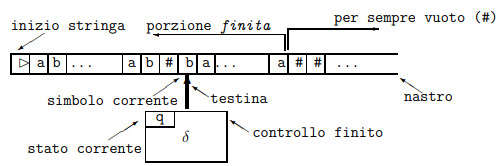
\includegraphics[scale=0.75]{mdt.png}
\end{center}
Mappatura a coda di rondine, bigezione tra (m, n) $\rightarrow$ k, cioè $N^2 \rightarrow N$.\\
Costruire un modello per il calcolo dopo aver posto delle condizioni affinché qualcosa si possa chiamare algoritmo.

\subsection{$\Sigma$}
\begin{list}{}{}
	\item $\Sigma^0$ = \{$\epsilon$\}, con $\epsilon =$ parola vuota, che non contiene caratteri
	\item $\Sigma^{i+1} = \Sigma \cdot \Sigma^i = \{\sigma \cdot u \:\:\vline\:\: \sigma \in \Sigma \:\wedge\: u \in \Sigma^i\}$
	\item $\Sigma^* = \bigcup_{i \in N}\sum^i$, insieme di tutte le possibili combinazioni di simboli
	\item $\Sigma^f = \Sigma^* \:\cdot\: (\Sigma \:-\: \{\#\} \:\bigcup\: \{\epsilon\})$, cioè l'insieme di tutte le stringhe che terminano con un carattere non bianco ma che possono terminare con la stringa vuota
\end{list}
\paragraph{Esempio} $\Sigma_B = \{0, 1\} \longrightarrow \Sigma_B^* = \{\epsilon, 0, 1, 01, 10, 010, 110010, \ldots\}$ tutti i numeri binari
\pagebreak
\subsection{Transizioni}
La \textbf{situazione corrente} di una macchina di Turing può essere scritto come $(q, u, \sigma, v)$ dove:
\begin{list}{}{}
	\item $q$ è lo \textbf{stato attuale}, $q \in Q$
	\item $u$ è la \textbf{stringa a sinistra} del carattere corrente, $u \in \sum^*$
	\item $\sigma$ è il \textbf{carattere corrente}, $\sigma \in \sum$
	\item $v$ è il \textbf{resto della stringa} che termina con un carattere non nullo, $v \in \sum^f$
\end{list}
Può anche essere più comodamente espressa come $(q, u \:\underline{\sigma}\: v)$

\subsection{Computazione}
Una computazione è una transizione $(q, x) \longrightarrow (q', \omega)$. Una macchina di Turing parte \textbf{sempre} da $(q_0, \underline{\triangleright} x)$.\\
Ogni computazione può esprimere il numero di passi necessari, ad esempio $\gamma \longrightarrow^n \gamma'$.\\
$\forall \:\:computazione\:\: \gamma \Rightarrow \gamma \longrightarrow^0 \gamma$. Inoltre se $\gamma \longrightarrow \gamma' \wedge \gamma' \longrightarrow^n \gamma''$ allora $\gamma \longrightarrow^{n+1} \gamma''$
\paragraph{Convergenza e divergenza} Diremo che la computazione $(q_0, w)\rightarrow^n(q',w')$ \textit{termina} (cioè \textbf{converge} $\downarrow$) $\Leftrightarrow q' = h$ e che \textit{non termina} (cioè \textbf{diverge} $\uparrow$) $\Leftrightarrow\:\forall\:q', w'\:|\:(q_0, w) \rightarrow^n (q', w')\:\exists\: q'', w''\:|\:(q', w')\rightarrow(q'', w'')$\\\\
Possiamo specificare la macchina M con cui eseguiamo la computazione con $\rightarrow^n_M$, usando M($w$) per specificare che la macchina M inizia la computazione da $(q_0,\underline{\triangleright}w)$, cioè che applichiamo M a $w$.
\paragraph{Esempio} Macchina di Turing che esegue la semplice somma di due semplici numeri romani.
\begin{multicols}{2}
\begin{center}
	\begin{tabular}{c | c | c}
		$q$ & $\sigma$ & $\delta(q, \sigma)$\\
		\hline
		$q_0$ & $\triangleright$ & $(q_0, \triangleright, R)$ \\
		$q_0$ & I & $(q_0, I, R)$ \\
		$q_0$ & $+$ & $(q_1, I, R)$ \\
		\hline
		$q_1$ & I & $(q_1, I, R)$ \\
		$q_1$ & \# & $(q_2, \#, L)$ \\
		\hline
		$q_2$ & I & $(h, \#, -)$ \\
	\end{tabular}
\end{center}
\columnbreak
$(q_0, \underline{\triangleright}II+III) \longrightarrow (q_0, \triangleright \underline{I}I+III) \longrightarrow (q_0, \triangleright I \underline{I}+III) \longrightarrow (q_0, \triangleright II \:\underline{+}\: III) \longrightarrow (q_1, \triangleright III\underline{I}II) \longrightarrow (q_1, \triangleright IIII \underline{I}I) \longrightarrow (q_1, \triangleright IIIII\underline{I}) \longrightarrow (q_1, \triangleright IIIIII\underline{\#}) \longrightarrow (q_2, \triangleright IIIII\underline{I}) \longrightarrow (h, \triangleright IIIII)$
\end{multicols}

\paragraph{Esempio} Macchina di Turing che verifica se una stringa di lettere $a, b$ è palindroma o no.
\begin{multicols}{2}
\begin{center}
	\begin{tabular}{c | c | c}
		$q$ & $\sigma$ & $\delta(q, \sigma)$\\
		\hline
		$q_0$ & $\triangleright$ & $(q_0, \triangleright, R)$ \\
		$q_0$ & $a$ & $(q_A, \triangleright, R)$ \\
		$q_0$ & $b$ & $(q_B, \triangleright, R)$ \\
		$q_0$ & $\#$ & $(h, \#, -)$ \\
		\hline
		$q_A$ & $a/b$ & $(q_A, a/b, R)$ \\
		$q_A$ & \# & $(q_{A'}, \#, L)$ \\
		\hline
		$q_{A'}$ & $a$ & $(q_R, \#, L)$ \\
		\hline
		$q_B$ & $a/b$ & $(q_B, a/b, R)$ \\
		$q_B$ & \# & $(q_{B'}, \#, L)$ \\
		\hline
		$q_{B'}$ & $a$ & $(q_R, \#, L)$ \\
		\hline
		$q_R$ & $a/b$ & $(q_R, a/b, R)$ \\
		$q_R$ & $\triangleright$ & $(q_0, \triangleright, R)$ \\
	\end{tabular}
\end{center}
\columnbreak
$(q_0, \underline{\triangleright}abba) \longrightarrow (q_0, \triangleright \underline{a}bba) \longrightarrow (q_A, \triangleright\triangleright \underline{b}ba) \longrightarrow \\ (q_A, \triangleright \triangleright b\underline{b}a) \longrightarrow (q_A, \triangleright \triangleright bb\underline{a}) \longrightarrow (q_A, \triangleright  \triangleright bba\underline{\#}) \longrightarrow \\ (q_{A'}, \triangleright \triangleright bb\underline{a}) \longrightarrow (q_R, \triangleright \triangleright b\underline{b}) \longrightarrow (q_R, \triangleright \triangleright \underline{b}b) \longrightarrow (q_R, \triangleright \underline{\triangleright} bb) \\ \longrightarrow (q_0, \triangleright \triangleright \underline{b}b) \longrightarrow (q_B, \triangleright \triangleright \triangleright \underline{b}) \longrightarrow (q_B, \triangleright \triangleright \triangleright b\underline{\#}) \longrightarrow \\ (q_{B'}, \triangleright \triangleright \triangleright \underline{b}) \longrightarrow (q_R, \triangleright \triangleright \underline{\triangleright})  \longrightarrow (h, \triangleright \triangleright \triangleright)$
\end{multicols}
\section{Linguaggi di Programmazione}
Un primo formalismo di algoritmo, come abbiamo visto, è la \textbf{macchina di Turing}: attenendosi alle richieste di tempo e spazio arbitrariamente grandi ma finiti, risolve un \textbf{problema}.\\
Un secondo formalismo sono i \textbf{linguaggi di programmazione}.
\subsection{Sintassi}
\paragraph{Sintassi astratta} Definiamo la \textbf{sintassi} dello scheletro di un semplice linguaggio di programmazione imperativo.\\
Una \textbf{sintassi astratta} è una sintassi non concreta, cioè che non tiene conto di alcune cose come la procedenza tra gli operatori.\\
\begin{list}{}{\textbf{Sintassi}}
	\item Expr $\rightarrow$ E ::= x $\vline\:$ n $\vline\:$ E + E $\vline\:$ E $\cdot$ E $\vline\:$ E - E
	\item Bexpr $\rightarrow$ B ::= tt $\vline\:$ ff $\vline\:$ E $<$ E $\vline\:$ $\neg$B $\vline\:$ B $\vee$ B
	\item Comm $\rightarrow$ C ::= \texttt{skip} $\vline\:$ x $=$ E $\vline\:$ C;C $\vline\:$ \texttt{if} B \texttt{then} C \texttt{else} C $\vline\:$ \texttt{for} i = E \texttt{to} E \texttt{do} C $\vline\:$ \texttt{while} B \texttt{do} C
\end{list}
\begin{list}{}{Abbiamo una serie di insiemi da definire ulteriormente}
	\item x $\in$ Var, l'insieme delle \textbf{variabili}
	\item n $\in$ $N$, \textbf{numeri naturali}.
\end{list}
\begin{list}{}{Abbiamo anche la \textbf{memoria} per poter \textbf{assegnare ad una variabile il suo significato}}
	\item $\sigma$ : Var $\rightarrow_{fin} N$\\
	Si dice "a dominio finito", indicata dal $fin$ sotto la freccia, per indicare che il dominio Var ha cardinalità finita. Var dominio è quindi un sottoinsieme di Var insieme delle variabili che sarebbe infinito.\\
	La memoria si può aggiornare, diventando $\sigma'$ = $\sigma[$x$\:\mapsto\:$n$]$.\\Ad esempio, $\sigma'(y)$ = n se y = x, altrimenti $\sigma'(y)$ = $\sigma(y)$
\end{list}
Chiameremo \texttt{WHILE} il linguaggio definito dalla grammatica BNF definita sopra, e \texttt{FOR} il linguaggio risultante dall'omissione del comando \texttt{while} B \texttt{do} C nella definizione.
\subsection{Funzioni di Valutazione}
\begin{list}{}{Inoltre, per valutare le espressioni generate dalla grammatica, servono delle \textbf{funzioni di valutazione}. Esse \textbf{trovano il significato di ogni espressione}}
	\item \textbf{Funzione di valutazione delle espressioni}\\$\mathscr{E}$ : Expr $\times$ (Var $\rightarrow N$) $\rightarrow N$\\La sua \textbf{semantica denotazionale} è la seguente
	\begin{multicols}{2}
	\begin{list}{}{}
		\item $\mathscr{E}[$x$]_\sigma$ = $\sigma$(x)
		\item $\mathscr{E}[$n$]_\sigma$ = n
		\item $\mathscr{E}[$E$_1$ $\pm$ E$_2]_\sigma$ = $\mathscr{E}[$E$_1]_\sigma$ $\pm$ $\mathscr{E}[$E$_2]_\sigma$
	\end{list}
	\end{multicols}
	Importante notare come gli operatori $+$, $-$, $\cdot$ \textit{dentro} le espressioni siano dei \textbf{semplici token denotazionali}, mentre sono gli operatori \textit{valutati} ad eseguire il vero e proprio calcolo. Per chiarire questo aspetto, facciamo un esempio. Valutiamo con la nostra funzione $\mathscr{E}[$E$_1$ $+$ E$_2]_\sigma$ = $\mathscr{E}[$E$_1]_\sigma$ \textit{più} $\mathscr{E}[$E$_2]_\sigma$. \textbf{Se non definiamo l'operatore} "\textit{più}", ponendo $\sigma$(x) = 25 la valutazione
	\begin{list}{}{}
		\item $\mathscr{E}[$3 + x$]_\sigma$ = $\mathscr{E}[$3$]_\sigma$ \textit{più} $\mathscr{E}[$x$]_\sigma$ = 3 \textit{più} 25 = 42
	\end{list}
	è corretta quanto
	\begin{list}{}{}
		\item $\mathscr{E}[$3 + x$]_\sigma$ = $\mathscr{E}[$3$]_\sigma$ \textit{più} $\mathscr{E}[$x$]_\sigma$ = 3 \textit{più} 25 = 28
	\end{list}
	Ovviamente utilizzeremo la valutazione specificata in precedenza e gli operatori aritmetici assumeranno il loro significato standard.\\
	L'unica eccezione è l'operatore $-$, che nel nostro caso sarà il \textbf{meno limitato} dal simbolo $\dot{-}$, la cui unica differenza è che non può dare un risultato inferiore a 0. Ad esempio, 5 $\dot{-}$ 7 = 0
	\pagebreak
	\item \textbf{Funzione di valutazione di espressioni booleane}\\$\mathscr{B}$ : Bexpr $\times$ (Var $\rightarrow N$) $\rightarrow$ \{tt, ff\}\\
	La cui \textbf{semantica denotazionale} è la seguente
	\begin{multicols}{2}
	\begin{list}{}{}
		\item $\mathscr{B}[$tt$]_\sigma$ = tt
		\item $\mathscr{B}[$ff$]_\sigma$ = ff
		\item $\mathscr{B}[$E$_1 <$ E$_2]_\sigma$ = $\mathscr{E}[$E$_1]_\sigma$ $<$ $\mathscr{E}[$E$_2]_\sigma$
		\item $\mathscr{B}[\neg$B$]_\sigma$ = $\neg\mathscr{B}[$B$]_\sigma$
		\item $\mathscr{B}[$B$_1 \vee$ B$_2]_\sigma$ = $\mathscr{B}[$B$_1]_\sigma$ $\vee$ $\mathscr{B}[$B$_2]_\sigma$
	\end{list}
	\end{multicols}
	Anche qua vale il medesimo discorso sulla definizione sugli effettivi operatori.
\end{list}
\subsection{Semantica Operazione Strutturale}
\paragraph{Structural Operationale Semantics} Metodo attraverso il quale viene fornita la semantica dei comandi. Parte da un \textbf{insieme di configurazioni $\Gamma$}
\begin{list}{}{}
	\item $\Gamma$ = \{(C, $\sigma$) $\vline\:$ FV(C) $\subset$ dom($\sigma$)\} $\cup$ \{$\sigma$\}
\end{list}
dove FV(C) sono le \textbf{variabili del programma} e con FV(C) $\subset$ dom($\sigma$) si richiede che tutte le variabili del programma abbiano un valore nella memoria fornita. Si fa l'unione con la sola memoria $\sigma$ perché la situazione finale è (  , $\sigma$) che, analogamente allo stato fittizio $h$ nella macchina di Turing, segnala la fine dell'esecuzione. Inoltre si hanno le \textbf{transizioni $\rightarrow$}
\begin{list}{}{}
	\item $\rightarrow \:\subset \Gamma \times \Gamma$
\end{list}
Definiamo quindi un \textbf{insieme di transizioni ($\Gamma$, $\rightarrow$)} tramite delle \textbf{regole di inferenza} del tipo $\frac{premesse}{conclusione}$. In assenza di premesse, $-$, la regola di inferenza si dice \textbf{assioma}.
\begin{multicols}{2}
	$$\frac{-}{(skip, \sigma) \rightarrow \sigma}$$
	$$\frac{-}{(x = E, \sigma) \rightarrow \sigma[x\:\mapsto\:n]}\textsl{ se }\mathscr{E}[E]_\sigma = n$$
	$$\frac{(C_1, \sigma) \rightarrow (C_1', \sigma')}{(C_1;C_2, \sigma) \rightarrow (C_1';C_2, \sigma')}$$
	$$\frac{-}{(if\:\: B\:\: then\:\: C_1\:\: else\:\: C_2, \sigma) \rightarrow(C_1, \sigma)}\textsl{ se }\mathscr{B}[B]_\sigma = tt$$
	$$\frac{-}{(if\:\: B\:\: then\:\: C_1\:\: else\:\: C_2, \sigma) \rightarrow(C_2, \sigma)}\textsl{ se }\mathscr{B}[B]_\sigma = ff$$
	$$\frac{-}{(for\:\: i = E_1\:\: to\:\: E_2\:\: do\:\: C, \sigma) \rightarrow \sigma}\textsl{ se }\mathscr{B}[E_2 < E_1]_\sigma = tt$$
\end{multicols}
	$$\frac{-}{(for\:\: i = E_1\:\: to\:\: E_2\:\: do\:\: C, \sigma) \rightarrow (i = n_1;\:\:C;\:\:for\:\: i = n_1 + 1\:\:to\:\:n_2\:\:do\:\:C, \sigma)}\textsl{ se }\mathscr{B}[E_2 < E_1]_\sigma = ff\: \wedge\: \mathscr[E_1]_\sigma = n_1 \wedge\: \mathscr[E_2]_\sigma = n_2$$
	$$\frac{-}{(while\:\:B\:\:do\:\:C, \sigma) \rightarrow (if\:\:B\:\:then\:\:C;\:\:while\:\:B\:\:do\:\:C,\sigma)} $$
\section{Calcolabilità}
\subsection{T-Calcolabile}
Dati $\Sigma$ alfabeto della macchina, $\Sigma_0$ alfabeto di input e $\Sigma_1$ alfabeto di output, con \#, $\triangleright \not\in \Sigma_0 \cup \Sigma_1 \subset \Sigma$
\begin{center}
M=(Q, $\Sigma$, $\delta$, q$_0$) calcola $f$ : $\Sigma_0^* \longrightarrow \Sigma_1^*$ $\Leftrightarrow$ ($\forall w \in \Sigma_0^* \wedge f(w) = z \Rightarrow M(w) \rightarrow_{fin}$ (h, $\triangleright z))$
\end{center}
Si dice che la \textbf{funzione} $f$ è \textbf{T-Calcolabile}.\\
Cioè, esiste una macchina di Turing che per ogni stringa finita in input arriva, con un numero finito di passi, all'arresto lasciando sul nastro la stringa di output corretta. Notare come non viene data nessuna interpretazione al risultato della $f$.
\subsection{\texttt{while}-Calcolabile}
\begin{center}
C calcola $f$ : Var $\rightarrow$ $N$ $\Leftrightarrow$ ($\forall\:\: \sigma$ : Var $\rightarrow$ $N$ $\wedge$ $f(x) = n$ $\Rightarrow$ C($\sigma$) $\rightarrow_{fin}$ $\sigma'$ $\wedge$ $\sigma'(x) = n$)
\end{center}
Si dice che la funzione $f$ è \textbf{\texttt{while}-Calcolabile}.\\
Cioè esiste un programma C che calcola il risultato corretto in un numero finito di passi.
\paragraph{Invariante} Tutti i risultati visti fin'ora \textbf{sono invarianti rispetto al modello dei dati}, e questo vale anche per la T-Calcolabilità e la \texttt{while}-Calcolabilità.\\
In particolare, se ho i dati in un formato A allora posso codificarli nel formato B in cui opera la macchina, calcolare il risultato in formato B e decoficarlo nel formato A di partenza. Questo vale se \textbf{le codifiche sono funzioni biunivoche e "\textit{facili}"}. Vedremo cosa significa essere "facili", ma per adesso basti pensare ad un numero finito di passi e che terminano sempre.
\subsection{Esempio di codifica}
\begin{multicols}{2}
\begin{center}
	\begin{tabular}{c || c | c | c | c | c | c}
	 & 0 & 1 & 2 & 3 & 4 & 5 \\
	 \hline
	 \hline
	 0 & 0 & 2 & 5 & 9 & 14 & \\
	 \hline
	 1 & 1 & 4 & 8 & 13 & & \\
	 \hline
	 2 & 3 & 7 & 12 & & & \\
	 \hline
	 3 & 6 & 11 & \ldots & & & \\
	 \hline
	 4 & 10 & 16 & & & & \\
	 \hline
	 5 & 15 & & & & & 
	\end{tabular}\\
	Codifica a coda di rondine
\end{center}
\paragraph{Codifica} ($x$, $y$) $\mapsto$ $\frac{1}{2}$($x^2 + 2xy + y^2 + 3x + y$)\\
Es. (3, 1) $\mapsto$ $\frac{1}{2}$($9 + 6 + 1 + 9 + 1$) = $\frac{26}{2}$ = 13
\paragraph{Decodifica} $n$ $\mapsto$ ($n - \frac{1}{2}k(k + 1)$, $k - (n - \frac{1}{2}k(k+1))$) con $k = \lfloor\frac{1}{2}(\sqrt{1 + 8n} -1)\rfloor$\\\\
Es 8 $\mapsto$ ($8 - 6$, $6 - 8 + 3$) = ($2$, $1$)\\
$k = \lfloor\frac{1}{2}\sqrt{1 + 8\cdot 8} - 1\rfloor = 3$\\
$\frac{k(k+1)}{2} = 6$
\end{multicols}
\section{Notazione}
Una \textbf{funzione} $f$ è $\subset$ A $\times$ B, con A spazio di partenza e B codominio. Quindi $f$(a) = b si può esprimere anche con (a, b) $\in$ $f$, con a $\in$ A e b $\in$ B.
\begin{list}{}{}
	\item $f$(a) = b $\wedge$ $f$(a) = c $\Rightarrow$ b = c
	\item Considereremo \textbf{funzioni parziali}, cioè funzioni con A contenente punti dove $f$ non è definita. Non è quindi detto che $\forall$ a $\in$ A $\exists$ b $\in$ B \vline $\:\:f$(a) = b
	\item $f$ \textbf{converge} su a, cioè $f$(a)$\downarrow$ $\Leftrightarrow$ $\exists$ b $\vline\:$ $f$(a) = b
	\item $f$ \textbf{diverge} su a, cioè $f$(a)$\uparrow$ $\Leftrightarrow$ $\not\exists$ b $\vline\:$ $f$(a) = b
	\item \textbf{Dominio} di $f$: $dom(f)$ = \{a \vline$\:\: f$(a)$\downarrow$\}
	\item \textbf{Immagine} di $f$: $imm(f)$ = \{b \vline$\:\: \exists$ a $\in$ A $\Rightarrow$ $f$(a) = b\}
\end{list}
\paragraph{Rapporto tra algoritmi A e funzioni $f$} $f$ è un \textbf{insieme potenzialmente infinito di coppie}, ma non posso assegnare due $f$ diverse allo stesso insieme, mentre esistono tanti algoritmi diversi che calcolano la stessa funzione.\\
Ad esempio, $f$ = $\emptyset$ è calcolata da \texttt{while(true) do skip} ma anche da \texttt{while(true) do skip;skip}.
\begin{enumerate}
	\item Quali sono le funzioni calcolabili?\\
	Nelle ipotesi iniziali di definizione di algoritmo, per adesso conosciamo le T-Calcolabili e le \texttt{while}-Calcolabili.
	\item Quali proprietà hanno?\\
	Posso combinarle?
	\item Esistono funzioni non calcolabili?
	\item Sono interessanti?\\
	Esistono a prescindere dalla macchina?
\end{enumerate}
\paragraph{Algoritmi e calcolabilità} Per ora abbiamo definito gli algoritmi in base al loro comportamento, sotto forma di \textbf{configurazioni che si susseguono} del tipo (istr. corrente + \ldots, memoria). Abbiamo anche diversi modi di affrontare la calcolabilità:
\begin{enumerate}
	\item \textbf{Hardware}, con la macchina di Turing\\
	Questo è uno dei primi esempi di calcolo, è semplice da capire e si descrivono direttamente macchine che eseguono gli algoritmi. Uno dei primi approcci allo studio della complessità.\\
	\textbf{Cambio programma $\rightarrow$ Cambio macchina}
	\item \textbf{Software}\\
	Ho l'interprete, cioè la semantica, fissi. Se cambio il programma non devo cambiare la macchina
	\begin{enumerate}
		\item Programmi \texttt{while}\\
		Base della programmazione iterativa, dalla semantica operazionale e anch'essi usati per lo studio della complessità
		\item Funzioni ricorsive\\
		Base della programmazione funzionale
	\end{enumerate}
\end{enumerate}

\section{Funzioni ricorsive primitive}
Per formalizzare i vari modi con cui possiamo esprimere le funzioni, usiamo quella che si chiama \textbf{$\lambda$-notazione}. Queste espressioni individuano gli argomenti all'interno di un'espressione che descrive una funzione, scritta seguendo un'opportuna sintassi.
$$\lambda <\textsl{variabili}>.<\textsl{espressione}>$$
\paragraph{Esempio} $\lambda\,x,\,y.\textsl{expr}$\\
Gli \textbf{argomenti} dell'espressione $\textsl{expr}$ sono $x$, $y$. Si dice anche che $x$, $y$ \textbf{appaiono legate da $\lambda$ in $\textsl{expr}$}.\\
Invece un qualsiasi altro simbolo di variabile $w$ in \textsl{expr} \textbf{non è da considerarsi argomento} dell'espressione, e viene definito \textbf{libero} in \textsl{expr}.\\
Altri \textbf{esempi} per evidenziare la \textbf{notazione}:
\begin{list}{}{}
	\item $\lambda\, y. x + y$
	\item $\lambda\, x \lambda\, y.x + y$ che può essere riscritta come $\lambda\, x,\,y.x + y$ ed equivale a dire $somma(x, y) = x + y$ dando così il nome $somma$ alla funzione.
	\item $\lambda\, x_1, x_2, \ldots, x_n.\textsl{expr}$ riscritta come $\lambda\, \overrightarrow{x}.\textsl{expr}$
\end{list}
\subsection{Classe C}
La classe $C$ delle \textbf{funzioni ricorsive primitive} è la \textbf{minima classe} di funzioni che obbediscono alle seguenti regole di inferenza, regole di sintassi per definire le funzioni.\\
\begin{list}{}{\textbf{Casi base}}
	\item \textbf{Zero}: $\lambda \overrightarrow{x}.0$\\
	Prende un vettore di argomenti e restituisce 0.
	\item \textbf{Successore}: $\lambda x.x+1$\\
	Prende un valore e restituisce il suo successore.
	\item \textbf{Proiezione}/\textbf{Identità}: $\lambda \overrightarrow{x}.x_i$\\
	$\overrightarrow{x} = x_1,\ldots, x_n$, $1 \leq i \leq n$
\end{list}
\begin{list}{}{\textbf{Casi iterativi}}
	\item \textbf{Composizione}\\
	$g_1,\ldots, g_n \in C$ con $k$ argomenti ("a $k$ posti") e\\
	$h \in C$ a $n$ posti\\
	$\Rightarrow \lambda x_1, \ldots, x_k.h(g_1(\overrightarrow{x}),\ldots, g_n(\overrightarrow{x})) \in C$
	\item \textbf{Ricorsione primitiva}\\
	$h \in C$ a $n + 1$ posti e\\
	$g \in C$ a $n - 1$ posti\\
	$\Rightarrow$
	$\left\{
		\begin{array}{l l l}
			f(0, x_2, \ldots, x_n)&= g(x_2, \ldots, x_n)&\textsl{Passo finale}\\
			f(x_1 + 1, x_2, \ldots, x_n)&= h(x_1, f(x_1, x_2, \ldots, x_n), x_2,\ldots, x_n)&\textsl{Iterazione}
		\end{array}
		\right.$
\end{list}
Questo rappresenta un \textbf{ciclo for}: $x_1$, la prima variabile di $f$, è il contatore da decrementare, $g$ è il passo finale e $h$ rappresenta i passi interni del ciclo. La terminazione è garantita, e si possono definire le primitive matematiche base con le funzioni ricorsive primitive.\\
$f \in C \Leftrightarrow$ esiste una successione $f_0,\ldots,\,f_n = f\:\:\vline\:\:\forall f_1$ è ottenuto con i casi base oppure $f_i$ è ottenuto con i casi iterativi da $f_j$ con $j < i$
\pagebreak
\paragraph{Esempio} Esempio di funzioni ricorsive\\
$f_1 = \lambda x.x$\\
$f_2 = \lambda x.x+1$\\
$f_3 = \lambda x_1, x_2, x_3. x_2$\\
$f_4 = f_2(f_3(x_1, x_2, x_3))$\\
\begin{math}
		\left\{
		\begin{array}{l}
			f_5(0, x_2) = f_1(x_2)\\
			f_5(x_1 + 1, x_2) = f_4(x_1, f_5(x_1, x_2), x_2)
		\end{array}
		\right.
\end{math}\\\\
Proviamo a calcolare $f_5(2, 3) =$
\begin{multicols}{2}
\textbf{Regola di valutazione interna-sinistra}: valuto per primo quello che sta dentro i parametri partendo da sinistra.\\
$f_5(2, 3) =$\\
$= f_5(1 + 1, 3) =$\\
$= f_4(1, \underline{f_5(1, 3)}, 3) =$\\
$= f_4(1, f_4(0, \underline{f_5(0, 3)}, 3), 3) =$\\$= f_4(1, f_4(0, \underline{f_1(3)}, 3), 3) =$\\
$= f_4(1,\underline{f_4(0, 3, 3)}, 3) =$\\
$= f_4(1, f_2(\underline{f_3(0, 3, 3)}), 3) =$\\
$= f_4(1, \underline{f_2(3)}, 3) =$\\
$= \underline{f_4(1, 4, 3)} =$\\
$= f_2(\underline{f_3(1, 4, 3)}) = $\\
$= \underline{f_2(4)} =$\\
$= 5$\\
\columnbreak

Vediamo cosa succede con una \textbf{regola di valutazione esterna}:\\
$f_5(2, 3) =$\\
$= \underline{f_4( 1, f_5(1, 3), 3)} =$\\
$= \underline{f_2(f_3(1, f_5(1, 3), 3))} =$\\
$= \underline{f_3(1, f_5(1, 3), 3)} + 1 =$\\
$= \underline{f_5(1, 3)} + 1 =$\\
$= \underline{f_4(0, f_5(0, 3), 3)} + 1 =$\\
$= \underline{f_2(f_3(0, f_5(0, 3), 3)} + 1 = $\\
$= \underline{f_3(0, f_5(0, 3), 3)} + 1 + 1 =$\\
$= \underline{f_5(0, 3)} + 2 =$\\
$= \underline{f_1(3)} + 2 =$\\
$= 3 + 2 =$\\
$= 5$
\end{multicols}

\begin{multicols}{2}
\paragraph{Meno Limitato} Non ritorna mai numeri negativi, ma 0.\\
$f_7(x, y) = y$\\\\
$f_8(x, y) = x$\\\\
\begin{math}
		\left\{
		\begin{array}{l}
			pred(0) = 0\\
			pred(x + 1) = f_8(x, pred(x))
		\end{array}
		\right.
\end{math}\\\\
$f_9(x, y, z) = pred(f_3(x, y, z))$\\\\
\begin{math}
		\left\{
		\begin{array}{l}
			f_{10}(0, y) = f_1(y)\\
			f_{10}(x + 1, y) = f_9(x, f_{10}(x, y), y)
		\end{array}
		\right.
\end{math}\\\\
$\Rightarrow x \dot{-} y = f_{10}(f_7(x, y), f_8(x, y))$
\columnbreak
\paragraph{Somma}
Non è altro che generalizzazione del successore, applico il successore tante volte quante servono.\\\\
\begin{math}
		\left\{
		\begin{array}{l}
			0 + y = y\\
			(x + 1) + y = (x + y) + 1
		\end{array}
		\right.
\end{math}
\paragraph{Prodotto}
Sfrutto la somma\\\\
\begin{math}
		\left\{
		\begin{array}{l}
			0 * y = 0\\
			(x + 1) * y = (x * y) + y
		\end{array}
		\right.
\end{math}
\paragraph{Potenza}
Generalizza il prodotto\\\\
\begin{math}
		\left\{
		\begin{array}{l}
			x^0 = 1\\
			x^{y + 1} = (x^y) * x\\
		\end{array}
		\right.
\end{math}\\\\
C'è un modo per generalizzare la potenza? $\Rightarrow$ \textbf{Ackerman}.
\end{multicols}

\paragraph{Relazione} Diciamo che la relazione $R(x_1,\ldots,\,x_n) \subset N^n$ è \textbf{ricorsiva primitiva} se lo è la sua \textbf{funzione caratteristica} $\chi_R$ definita come\\
\begin{math}
\chi_R(x_1,\ldots, x_n) = 
		\left\{
		\begin{array}{l}
			1 \:\:\:\:\textsl{se}\:\: (x_1, \ldots, x_n) \in R\\
			0 \:\:\:\:\textsl{se}\:\: (x_1, \ldots, x_n) \not\in R
		\end{array}
		\right.
\end{math}\\\\
Quindi se $\chi_R$ è ricorsiva primitiva allora anche $R$ è ricorsiva primitiva. Come esempio, vediamo l'uguaglianza:
$$\chi_=(0, 0) = 1\:\:\:\:\chi_=(x+1, y+1)=\chi_=(x,y)\:\:\:\:\chi_=(0, y+1)=0\:\:\:\:\chi_=(x+1,0)=0$$

\paragraph{Esempio} $P =$ \{ $n \in N\:\:\vline$ $n$ è un numero primo\} è ricorsiva primitiva. Questo per il teorema di fattorizzazione unica.\\
$\forall x \in N\:\:\exists$ numero finito di esponenti $x_1 \neq 0\:\:\vline\:\: x = p_0^{x_0}\cdot p_1^{x_1}\cdot\ldots\cdot p_n^{x_n}$\\
Come trovare tali esponenti con $f$ ricorsiva primitiva.\\
M = (Q, $\Sigma$, $\delta$, q$_0$)\\
Q = \{q$_0$, \ldots, q$_k$), $\Sigma$ = \{$\sigma_0$, \ldots, $\sigma_n$)
\pagebreak
\subsection{Numerazione di Godel} 
\textbf{Kurt G\"{o}del}, rappresentare algoritmi come numeri: \textbf{G\"{o}delizzazione}, cioè data una MdT M trovo $i$ che è il suo \textbf{numero di G\"{o}del}.\\
La funzione caratteristica dell'insieme dei numeri primi è ricorsiva primitiva. Gli esponenti della fattorizzazione in numeri primi di qualsiasi numero naturale sono dati da funzioni ricorsive primitive.\\
Ne deriva che ogni sequenza di numeri naturali può essere codificata come numero naturale, usando i numeri come esponenti della fattorizzazione in numeri primi. \textbf{Questa codifica è iniettiva ma non suriettiva}, e una codifica effettiva deve essere anche suriettiva. G\"{o}del fornì una migliore codifica che era anche suriettiva, da cui deriva che le funzioni di codifica e decodifica sono ricorsive primitive. Tutte le MdT, programmi \texttt{for}/\texttt{while}, funzioni ricorsive primitive e $\mu$-ricorsive possono essere effettivamente codificate e decodificate come numeri naturali, usando i simboli sintattici come numeri naturali distinti. Le computazioni (intese come successioni di configurazioni) possono anch'esse essere codificate e decodificate.\\\\
Data M = (Q, $\sum$, $\delta$, $q_0$) MdT con Q = \{$q_0$, \ldots, $q_n$\} e $\sum$ = \{$\sigma_0$, \ldots, $\sigma_m$\}, ogni quintupla $(q_i, \sigma_j, q_k, \sigma_l, D)\in\delta$ è codificata come $p_0^{i+1}\cdot p_1^{j+1}\cdot p_2^{k+1}\cdot p_3^{l+1}\cdot p_4^{m_D}$ con $p_0<\ldots<p_4$ sono numeri primi. Se consideriamo i simboli di direzione come simboli veri e propri, allora L = $\sigma_{m+2}$, R = $\sigma_{m+3}$, --- = $\sigma_{m+4}$ e poniamo $m_D\in\{m_L=m+2, m_R=m+3, m_-=m+4\}$\\\\
Grazie al teorema della fattorizzazione unica, ad ogni quintupla è associato un solo intero e viceversa, che rende la funzione iniettiva.\\
Possiamo ordinare l'insieme delle quintuple che caratterizza M, ottenendo una successione di quintuple codificate con un numero: abbiamo una successione $a_0a_1\ldots a_n$ di numeri naturali tali che $a_i\neq a_j$ se $i\neq j$. Codificando questa successione otteniamo un altro numero, $i$ detto \textbf{indice associato alla MdT M}.\\\\
La funzione non è suriettiva, ma il problema può essere aggirato: decodificando $i$, se ottengo una MdT bene, altrimenti $i$ non è un indice e lo butto, oppure restituisco un valore speciale.\\\\
Tutte le funzioni definibili mediante gli schemi di ricorsione primitiva sono totali, e data una funzione ricorsiva primitiva si può scrivere un programma \texttt{FOR} che dati gli stessi argomenti produce lo stesso risultato, e viceversa.\\
Abbiamo trovato il formalismo definitivo, che esprime tutte le funzioni calcolabili? \textbf{No}, perché esiste la funzione di Ackermann: totale, con una definizione accettabile ma che non è definibile mediante gli schemi di ricorsione primitiva.
\subsection{Funzione di Ackermann}
La funzione di Ackermann \textbf{non è definibile} mediante gli schemi di ricorsione primitiva definiti in precedenze, ma è totale ed ha una definizione intuitivamente accettabilissima.

\begin{list}{}{}
	\item $A(0, 0, y) = y$
	\item $A(0, x + 1, y) = A(0, x, y) + 1$
	\item $A(1, 0, y) = 0$
	\item $A(z + 2, 0, y) = 1$
	\item $A(z + 1, x + 1, y) = A(z, A(z + 1, x, y), y)$ \textbf{doppia ricorsione}

\end{list}
La \textbf{doppia ricorsione} presente non è un problema: tutti i valori su cui si ricorre decrescono, quindi i valori di $A(z, x, y)$ sono definiti in termini di un numero finito di valori della funzione $A$. Quindi intuitivamente $A$ è calcolabile. Inoltre \textbf{cresce più rapidamente di ogni funzione ricorsiva primitiva} ma \textbf{non è ricorsiva primitiva}.\\
Ma cosa calcola? Una sorta di esponenziale generalizzato, infatti:
\begin{list}{}{}
	\item $A(0, x, y) = y + x$
	\item $A(1, x, y) = y * x$
	\item $A(2, x, y) = y^x$
	\item $A(3, x, y) = y^{\left.y^{\ldots^y}\right\} \:x\:\textsl{volte}}$
\end{list}
\pagebreak
\subsection{Realizzazione}
Con il linguaggio-\texttt{while} e il linguaggio-\texttt{for} posso riprodurre i casi base della ricorsione. In particolare, per ogni programma \texttt{for} esiste una funzione ricorsiva primitiva e viceversa.\\
\begin{list}{}{}
	\item Un programma che calcola lo $0$ è un programma che legge gli ingressi e scrive $0$ in uscita.
	\item Il successore lo realizzo con un assegnamento uscita $=$ ingresso $ + 1$
	\item La proiezione consiste nel leggere in memoria la variabile $x_i$ cercata e metterla in uscita
	\item Realizzo $h$ tale che $h(g_1(x, y, z), g_2(x, y, z))$, con programma $p_1$ associato a $g_1$, $p_2$ associato a $g_2$ e $p_3$ associato a $h$.\\
Il programma che realizza la composizione sarà quindi $p_1$;$p_2$;$p_3$.\\
	\item Per la ricorsione primitiva
	\begin{math}
		\left\{
		\begin{array}{l}
			f(0, y) = g(y) \rightarrow p_1\\
			f(x + 1, y) = h(x, f(x, y), y) \rightarrow p_2
		\end{array}
		\right.
	\end{math}
	che dopo qualche passaggio abbiamo visto che\\$f(x + 1, y) =  h(x, f(x, y), y) = h(x, h(x + 1, f( x + 1, y)), y)$. Associando $p_1$ a $g$ e $p_2$ a $h$, lo realizzo con il programma-\texttt{for}
	\begin{lstlisting}
t1 = g(y);
for (i = 1 to x + 1):
	t1 = g(i, t1, y);
end
	\end{lstlisting}
\end{list}
Per la \textbf{funzione caratteristica} $\chi_I(n) =$
\begin{math}
		\left\{
		\begin{array}{l}
			1\:\: n \in I\\
			0\:\:\textsl{altrimenti}
		\end{array}
		\right.
\end{math}
\section{Diagonalizzazione}
\paragraph{Esiste un formalismo che esprime tutte e sole le funzioni totali calcolabili?} \textbf{No}\\
Dobbiamo necessariamente avere a che fare con funzioni parziali, ma perché "no"?\\
\textbf{Qualunque formalismo o esprime solo funzioni totali ma non tutte, oppure esprime anche funzioni parziali}. La dimostrazione è fondamentale per la teoria della calcolabilità: prende il nome di \textbf{diagonalizzazione}.
\subparagraph{Dimostazione} Fissato il formalismo delle funzioni ricorsive primitive, posso prendere l'algoritmo di G\"{o}del per numerarle: avrò le funzioni $f_0$, $f_1$, \ldots, $f_n$, \ldots così numerate.\\
Definisco $g(n) = f_n(n) + 1$ (\textit{diagonalizzazione} viene da usare lo stesso indice per indice e parametro): effettivamente calcolabile perché basta prendere l'algoritmo $n$-esimo, applicarlo a $n$ e sommare 1 al risultato. Inoltre, $g$ è totale.\\
Se $g$ è una ricorsiva primitiva, allora è numerabile: diciamo che $g$ ha come numero $i$, cioè $f_i(n) = g(n) = f_n(n) + 1$\\
Se diagonalizzo avrò $f_i(i) = g(i) = f_i(i) + 1$ ma \textbf{non può succedere} che $f_i(i) = f_i(i) + 1$\\
$\Rightarrow g$ non è ricorsiva primitiva.\\\\
Se io prendo le funzioni parziali, posso applicare lo stesso ragionamento?\\
$\phi(x) = \psi_x(x) + 1$\\
Diciamo come prima che $\phi(x)$ ha indice $i$, quindi $\psi_i(x) = \phi(x) = \psi_x(x) + 1$\\
Se $\psi_i(x)$ diverge, allora $\psi_x(x)$ diverge e anche $\psi_x(x) + 1$ diverge, quindi sono uguali. Non si applica il ragionamento della diagonalizzazione nel caso delle funzioni parziali.\\
Quindi il discorso \textbf{si applica ad ogni formalismo che definisca solo funzioni totali}.
\section{$\mu$-ricorsive}
Minima classe $\mathscr{R}$ che, allo schema fino alla ricorsione primitiva, aggiunge:
\paragraph{Minimizzazione} $\phi(\overrightarrow{x}, y) \in \mathscr{R}$\\
$\psi(\overrightarrow{x}) = \mu y.[\phi(\overrightarrow{x}, y) = 0 \wedge \forall z \leq y\:\:\vline\:\: \phi(\overrightarrow{x}, z)\downarrow] $\\\\
$\mu x.[I]$ è il minimo elemento di $I$ insieme.
\pagebreak
\paragraph{} Cosa significa? Data una funzione $\phi \in \mathscr{R}$ (che ovviamente può essere una ricorsiva primitiva), la vado a calcolare sugli argomenti $\overrightarrow{x}$ della $\psi$ e su una certa $y$. Se vale 0, il risultato è $y$, altrimenti \textbf{deve} convergere e vado avanti incrementando $y$ di 1 e ricalcolando fino a che non trovo un risultato pari a 0.\\
Quindi le $\mu$-ricorsive definiscono anche funzioni non totali, al contrario delle ricorsive primitive che definiscono solo funzioni totali.\\
La $\mu$ corrisponde ad un \textbf{ciclo while}: inizia con $y=0$ e lo incrementa fino a che $\phi$ non è uguale a 0 (guardia del loop), ritornando $y$. Se viene piazzato un limite superiore a $y$, allora $\psi$ potrebbe essere ricorsiva primitiva e se lo è anche la $\phi$ allora la condizione di convergenza è garantita.\\
La diagonalizzazione non può essere applicata direttamente alle funzioni $\mu$-ricorsive, perché $\phi_n(n)$ può divergere. Non tutte le funzioni $\mu$-ricorsive possono essere estese a funzioni totali: \textbf{una funzione è $\mu$-calcolabile se può essere ridefinita come $\mu$-ricorsiva}.
\subparagraph{Esempio} $\phi(x, y) = 42$ è costante, quindi ricorsiva primitiva, quindi anche $\mu$-ricorsiva.\\
$\psi(x) = \mu y.[\phi(x, y) = 42]$ ovunque indefinita perché non tornerà mai 0 quindi $\not\exists\:y$.\\\\
Quindi \textbf{terminazione e non terminazione sono cruciali}.\\
Se la definisco per casi? Ad esempio 
\begin{math}
	f(x) = \left\{
	\begin{array}{c c}
	\mu y.[y < g(x)\:\:\vline\:\: h(x, y) = 0] & \textsl{se}\:\exists\:\textsl{tale}\:y\\
	0 & \textsl{altrimenti}
	\end{array}
	\right.
\end{math}
con $g$, $h$ ricorsive primitive.\\$f$ è ricorsiva primitiva, perché composizione di ricorsive primitive, ed è anche totale, perché converge sempre.\\
Quindi \textbf{se pongo dei limiti al numero di tentativi}, dato da $y < g(x)$, si ricade nelle ricorsive primitive e non ci sono problemi di parzialità.
\subsection{Notazione}
Per ragioni storiche, una relazione $I \subset N^n$ è \textbf{ricorsiva} (sinonimo di totale) $\Leftrightarrow$ la sua funzione caratteristica $\chi_I$ è \textbf{calcolabile totale}.\\
Inoltre, come già detto, $I$ è ricorsiva primitiva $\Leftrightarrow$ $\chi_I$ è ricorsiva primitiva.
\section{Tesi di Church-Turing}
\textbf{Le funzioni intuitivamente calcolabili sono tutte e sole le T-calcolabili}.\\
In realtà è un'ipotesi, ma è così forte che viene presa come tesi. Ci permette di non considerare il formalismo con cui formalizziamo gli algoritmi, poiché tutti i formalismi rappresentano la stessa \textit{classe di elementi}. Ci limiteremo a dire algoritmo, Macchina di Turing\ldots$\,$ indifferentemente, poiché grazie a questa tesi possiamo dire che un algoritmo è equivalente qualsiasi sia il linguaggio in cui è scritto.\\
Questa tesi postula che la nozione di calcolabilità \textit{intuitiva} è robusta, ma cade se si rilascia anche una sola delle ipotesi fatte sulla natura degli algoritmi.\\\\
Da qui in avanti parleremo di \textbf{funzioni calcolabili} senza specificare il formalismo con cui le definiamo.\\
Quante sono? Ce ne sono di non calcolabili? Se ce ne sono, sono interessanti?
\subsection{Risultati}
Indichiamo con $\phi_i$ è la \textbf{funzione calcolata dall'$i$-esimo algoritmo} M$_i$
\begin{list}{}{}
	\item $\phi_i$ è funzione $\rightarrow$ \textbf{semantica}
	\item M$_i$ è algoritmo $\rightarrow$ \textbf{sintassi}
\end{list}
Può succedere per $i \neq j$ che $\phi_i = \phi_j$ ma M$_i \neq$ M$_j$ (ad esempio \texttt{while(true) do skip} e \texttt{while(true) do skip;skip}).
\begin{center}
T-calcolabili $=$ \texttt{while}-calcolabili $=$ $\mu$-calcolabili
\end{center}
D'ora in avanti parliamo solo di funzioni calcolabili, quindi $\phi_i$ \textit{è} calcolabile.
\paragraph{Tempo di calcolo} $\exists$? una funzione calcolabile totale $t(i, n)$ che maggiora il tempo di calcolo di M$_i$(n)? No. Vediamo come dimostrarlo, introducendo una \textbf{diagonalizzazione}.\\
$t(i, n)$ = \begin{math}
\left\{
\begin{array}{l l}
	k & \text{se }M_i(n)\downarrow \text{in meno di }i\text{ passi}\\
	0 & \text{altrimenti}
\end{array}
\right.
\end{math}\\
Sia T$_i$ la misura \textbf{esatta} del tempo di calcolo di M$_i$. T$_i$(n) $\leq$ $t(i, n)$ è calcolabile totale e $T_x(x)$ \textbf{tempo di calcolo effettivo}, $t(x, x)$ \textbf{tempo di calcolo stimato}\\
$\psi(x) = $
\begin{math}
\left\{
\begin{array}{l l}
	\phi_x(x) + 1 & \text{se }T_x(x) \leq t(x, x)\\
	0 & \text{altrimenti}
\end{array}
\right.
\end{math}\\
Quindi anche $\psi$ è calcolabile totale. Applico Church-Turing, quindi $\phi_i(i) = \psi(i) =$ \begin{math}
\left\{
\begin{array}{l l}
	\phi_i(i) + 1 & \text{se }T_i(i) \leq t(i, i)\\
	0 & \text{altrimenti}
\end{array}
\right.
\end{math}\\
Ma siccome $\phi_i$ è calcolabile totale, non può succedere che, quando termina, sia $\phi_i(i) = \phi_i(i) + 1$, \textbf{è un assurdo}. Quindi $t(i, n)$ non è calcolabile totale, di conseguenza \textbf{non c'è modo di stimare il tempo di calcolo}.\\
Per lo stesso motivo non possiamo imporre limiti allo spazio.
\paragraph{Spazio di calcolo} $\exists$? una funzione calcolabile totale che dato M$_i$, $x$ dice quante celle di memoria uno specifico calcolatore C userà per calcolare M$_i(x)$?\\
$h(i, x) = $\begin{math}
\left\{
\begin{array}{l l}
	1 & \text{se }M_i(x)\uparrow (\text{su }C)\\
	0 & \text{altrimenti}
\end{array}
\right.
\end{math}\\
Sia $n$ la cardinalità di $\Sigma$, $m - 1$ cardinalità di $Q$ e $k$ il numero di celle di C.\\
Posso quindi scrivere $n^k$ \textbf{stringhe diverse}: il cursore può stare su $k$ posizioni diverse e la macchina in $m$ stati diversi.\\
Il \textbf{numero massimo di configurazioni diverse} (stato con posizione del cursore e stringa su nastro) è  $l = n^k \cdot k \cdot m$, con $n^k$ possibilità di nastro scritto, $k$ possibili posizioni del cursore e $m$ stati ($m - 1$ + $1$ per lo stato $h$ di \textbf{halt})\\
Dopo $l$ passi, quindi, la configurazione si ripete necessariamente. Si può dire che \textbf{la macchina è in loop}.\\
Siccome la macchina attraversa un \textbf{numero finito di configurazioni superiormente limitato da} $l$, se la macchina non si è arrestata prima di $l$ passi allora troverò per forza una configurazione già vista in precedenza, che mi porterà in una configurazione già vista e così via. \textbf{Quindi non terminerà mai}.\\
Ho dimostrato che $h$ è calcolabile totale, ma posso scrivere quindi $t$ come nella dimostrazione precedente, ma giungo all'assurdo già visto. \textbf{Quindi non posso mettere un limite al nastro.}\\\\
I seguenti risultati sono \textbf{invarianti rispetto all'enumerazione scelta}.
\subsection{Teorema 1: Le Funzioni Calcolabili sono tante quante i numeri naturali}
Le $f$ calcolabili sono \#$N$. Anche le $f$ calcolabili totali sono \#$N$.\\
Esistono funzioni \textit{non} calcolabili, molte di più di quelle calcolabili.
\paragraph{Dimostrazione} Sono almeno \#$N$ perché posso costruire una macchina che per qualsiasi input lascia un numero naturale sul nastro, quindi di queste ce ne sono almeno quanti sono i numeri naturali. Non sono più di \#$N$ perché le MdT si possono enumerare (es. G\"{o}del).\\\\
Quindi indichiamo con $\phi_i$ la funzione (in generale, parziale) calcolata dall'algoritmo M$_i$ e $i$ \textbf{indice della macchina}. Come detto prima, può darsi che per $i \neq j$ sia $\phi_i = \phi_j$ ma sicuramente M$_i \neq$ M$_j$.
\subsection{Teorema 2: Ogni funzione calcolabile $\phi_i$ ha infiniti (numerabili) indici}
Anche detto \textbf{padding lemma}.\\
Non solo, posso costruire un insieme infinito di indici A$_i$ tale che $\forall\:j \in$ A$_i \Rightarrow \phi_j = \phi_i$ mediante una funzione ricorsiva primitiva.
\paragraph{Dimostrazione} Sia $M_i$ un programma \texttt{P}. Prendo \texttt{P;skip}, poi \texttt{P;skip;skip}\ldots metto tanti \texttt{;skip} quanti voglio. Posso generare un numero infinito di programmi che calcolano tutti la stessa funzione.
\subsection{Teorema 3: Forma Normale}
Prendendo un qualsiasi algoritmo, posso riscriverlo in una \textbf{forma canonica}/\textbf{normale}, che non è per forza migliore ma è una forma specifica e da noi \textbf{privilegiata}.\\
$\exists$ un predicato $T(i, x, y)$ e una funzione $U(y)$ ricorsive primitive calcolabili totali tali che $\forall$ funzione calcolabile $i$, $x$.$\phi_i(x)$ = $\mu$y.[$U(T(i, x, y))$]
\paragraph{Dimostrazione} Devo costruire il predicato T e la funzione U.\\
$T(i, x, y)$ è detto \textbf{predicato di Kleene} ed è \textbf{vero $\Leftrightarrow$ $y$ è la codifica di una computazione di M$_i$($x$) terminante}.\\
Per calcolare, $T$ prende $i$ e recupera M$_i$. Comincia a scandire i valori $y$, li decodifica e, uno alla volta dato $x$ ingresso, controlla se il risultato è una computazione terminante. Definisce $U$ in modo che $U(y) = z$, con $z$ risultato della computazione (ciò che rimane sul nastro della MdT corrispondente, cioè la macchina terminante M$_i$($x$) = $c_0c_1\ldots c_n$ con $c_n=(h,\triangleright z \underline{\#})$).\\
C'è un solo $y$ nelle macchine deterministiche, se c'è, quindi T e U sono calcolabili per la tesi di Church-Turing. Inoltre il procedimento termina sempre, quindi T e U sono totali.\\
Se considerassimo le MdT non deterministiche, potrebbero esserci più computazioni che terminano in $h$, per cui $\mu$ (l'operatore di minimizzazione) darebbe come risultato il minimo intero che ne codifica una.\\\\
Un immediato \textbf{corollario} del teorema di forma normale è che tutte le funzioni T-calcolabili sono anche $\mu$-calcolabili. Non solo, ma $\mu$y corrisponde al \texttt{while}, e $T$, $U$ a due programmi \texttt{for}. Quindi ogni funzione calcolabile può essere ottenuta da due programmi scritti con il linguaggio \texttt{for} ed una sola applicazione del linguaggio \texttt{while}.
\subsection{Teorema 4: Teorema di enumerazione}
$\exists\: z\:|\:\forall$ $i$, $x\:\:\:\phi_z(i, x) = \phi_i(x)$. Quindi $z$ è \textbf{MdT universale}. $z$ interprete, $i$ è programma.\\
Fra tutti gli algoritmi, ce ne sono infiniti numerabili in grado di eseguire tutti gli altri algoritmi.\\
\paragraph{Dimostrazione} $\phi_i(x) = \mu y.U(T(i, x, y))$ per il terzo teorema. Quindi $\phi_i(x)$ è un algoritmo, avrà un indice per Church-Turing che indicheremo con $z$.\\
Diciamo $\phi_i(x) = \phi_z(i, x) = \mu y.U(T(i, x, y))$ (senza $y$ come argomento perché quantificata, non libera ma legata, una sorta di \textit{variabile di lavoro}). Applico la transitività dell'uguaglianza e ho finito, $\phi_i(x) = \phi_z(i, x)$.\\
Più intuitivamente: M$_z$ recupera la descrizione di M$_i$ e la applica a $x$.
\section{Macchina di Turing Universale}
Ottimo modello per le macchine Von Neumann.
\paragraph{Due insiemi} Utili per la rappresentazione\\
$Q_* = \{q_0, q_1, \ldots\} \not\ni h$, insieme numerabile: \textbf{non è l'insieme degli stati} della MdTU ma è un insieme ausiliario.\\
$\Sigma_* = \{\sigma_0, \sigma_1, \ldots\} \not\ni L, R, -$ insieme di simboli.\\
Ogni MdT M$_k$ ha l'insieme degli stati $Q_k$ e quello dei simboli $\Sigma_k$ inclusi rispettivamente in $Q_*$ e $\Sigma_*$
\paragraph{Codifica K} $K : Q_* \cup \{h\} \cup \Sigma_* \cup \{L, R, -\} \rightarrow \{\:\vline\:\}^*$\\
Ognuno degli elementi $q_i$, $\sigma_i$ ecc. viene codificato in questo modo.\\
$h \mapsto\:\:\vline$\\
$q_i \mapsto\:\:\vline^{i + 2}$, con la barra verticale ripetuta $i + 2$ volte\\
$L \mapsto\:\:\vline$, $R \mapsto\:\:\vline\:\vline$, $- \mapsto\:\:\vline\:\vline\:\vline$\\
$\sigma_i \mapsto\:\:\vline^{i + 4}$\\
C'è un problema: $\vline\:\vline\:\vline\:\vline\:\vline$ è uno stato ($\in Q_*$) o un simbolo ($\in \Sigma_*$)? Vedremo come disambiguare.\\
$K$ non è biunivoca, ma lo è quando sappiamo se la stringa da decodificare è uno stato, un simbolo o una direzione: separeremo la codifica degli stati da quella dei simboli e delle direzioni da una marca $c$ \textbf{non appartenente all'alfabeto della macchina da decodificare}.\\
$Q_*$ contiene \textbf{tutti i possibili stati delle MdT}, e $\Sigma_*$ contiene \textbf{tutti i possibili simboli delle MdT}. Quanto visto fin'ora è ausiliario alla costruzione della MdTU.
\paragraph{Costruzione} Prendo una MdT qualunque $M = (Q, \Sigma, \delta, s)$. Ordiniamo gli stati ed i simboli.\\
$Q = \{q_{i_1}, q_{i_2}, \ldots, q_{i_k}\}$, finito perché gli stati sono finiti.\\
$\Sigma = \{\sigma_{j_1}, \sigma_{j_2}, \ldots, \sigma_{j_l}\}$.\\
Con $i_1 < i_2 < \ldots < i_k$ e $j_1 < j_2 < \ldots < j_l$. Con questo abbiamo supposto $Q$ e $\Sigma$ \textbf{totalmente ordinate}.\\
Considero questo alfabeto: $\{\:\vline\:, c, d, \#, \triangleright\}$ con $\vline\:, c, d \not\in Q_* \cup \Sigma_*$.\\
Adesso possiamo codificare le quintuple $\in \delta$. $\delta(q_{i_p}, \sigma_{j_q}) = (q, \sigma, D)$ con $D$ un certo simbolo di direzione ($L, R, -$). Come codificarla? Attraverso la seguente stringa
$$s_{p,q} = cK(q_{i_p})cK(\sigma_{j_q})cK(q)cK(\sigma)cK(D)c$$
con $c$ che funge da \textbf{separatore}, \textbf{tra la codifica di uno stato e la codifica di un simbolo}.\\
$s_{p,q} = cK(q_{i_p})cK(\sigma_{j_q})cdcdcd$ se $\delta(q_{i_p}, \sigma_{i_q})$ è indefinita
\pagebreak
\paragraph{Esempio} $\overline{M} = \{\{q_2\}, \{\sigma_1, \sigma_3, \sigma_5\}, \delta, q_2\}$, con $i_1 = 2$, $j_1 = 1$, $j_2 = 3$, $j_3 = 5$
\begin{list}{}{}
	\item $q_2 \rightarrow q_{i_1}$
	\item $\sigma_1 \rightarrow \sigma_{j_1}$
	\item $\sigma_3 \rightarrow \sigma_{j_2}$
	\item $\sigma_5 \rightarrow \sigma_{j_3}$
\end{list}
$\delta(q_2, \sigma_1) = (h, \sigma_5, -) \mapsto s_{1, 1} = c|^4c|^5c|c|^9c|^3c$ perché $K(q_2) = |^{2 + 2}$, $K(\sigma_1) = |^{1 + 4}$, $K(h) = |$, $K(\sigma_5) = |^{5 + 4}$, $K(-) = |||$ \\
$\delta(q_2, \sigma_3) = (q_2, \sigma_1, R) \mapsto s_{1, 2} = c|^4c|^7c|^4c|^5c|^2c$\\
$\delta(q_2, \sigma_5)$ non definita $\mapsto s_{1, 3} = c|^4c|^9cdcdcdc$
\paragraph{Codifica della macchina $\rho$} Possiamo ora definire una funzione di "\textit{codifica}" (in realtà iniettiva, perché in fase di decodifica possiamo non trovare una M corrispondente) della macchina in esame. ($s$ senza indici è lo stato iniziale)\\
$\rho(M) = cK(s)cs_{1,1}s_{1_2}\ldots s_{1,l}c\ldots cs_{k,1}s_{k_2}\ldots s_{k,l}c$\\
Praticamente si mettono "in coda" tutte le codifiche dei $\delta($stato$, $simbolo$) \rightarrow s_{stato, simbolo}$, separando con $c$ il "cambio" dello stato.\\
$\rho(M) = c <$codifica di $s>c<$codifiche dello stato $1$ per simbolo$>c\ldots c<$codifiche dello stato $k$ per simbolo$>c$\\\\
$\rho(M(w)) = \rho(M)\tau(w)$ con $\tau(\sigma_0', \ldots, \sigma_n') = cK(\sigma_0')cK(\sigma_1')c\ldots cK(\sigma_n')c$
\paragraph{Esempio} $\rho(\overline{M}) = c|^4c\:\:c|^4c|^5c|c|^9c|^3c\:\:c|^4c|^7c|^4c|^5c|^2c\:\:c|^4c|^9cdcdcdc\:\:c$\\\\
Dato che $\exists\:z\:\:\vline\:\:\forall\:i,x$ si ha $\phi_z(i, x) = \phi_i(x)$, allora vogliamo che la MdTU si comporta esattamente come $\overline{M}$ quando codifica $\overline{M}$. Quindi
\begin{list}{}{}
	\item $(s, \underline{\triangleright}w) \longrightarrow_n^M (h, u\underline{a}v) \Rightarrow (s_U, \underline{\triangleright}\rho(M)\tau(w)) \longrightarrow_m^U (h, \tau(uav)\underline{\#})$
	\item $(s_U, \underline{\triangleright}\rho(M)\tau(w)) \longrightarrow_n^U (h, u'a'v')$ dovrebbe succedere che $a' = \#$ e $v' = \epsilon$, ma anche che $u' = \tau(uav)$. Se succede\\$\Rightarrow (s, \underline{\triangleright}w) \longrightarrow_m^M (h, uav)$
\end{list}
\section{Teoremi}
\subsection{Teorema del parametro (s--m--n)}
$\exists$ $s$ calcolabile, totale, iniettiva $\vline$ $\forall$ $i$, $x$ $\lambda y.\phi_i(x, y) = \phi_{s(i, x)}(y)$\\
Quindi considerato $x$ come parametro, la funzione può essere calcolata da un'altra macchina di indice dipendente da $i$ e $x$. Ottimo strumento per dimostrare diversi risultati.\\
Intuitivamente, il programma $P_{s(i, x)}$ opera su $y$ soltanto mentre $P_i$ opera su $x$ e su $y$. Quindi $x$ è un \textbf{parametro} di $P_i$. Da $P_i(x,y) \rightarrow j = s(i, x)\:|\:P_j(y) = P_i(x,y)$\\\\
Al caso generale, $\forall\:m, n > 0\:\:\:\:\exists\:s_n^m$ calcolabile, totale e iniettiva con $m+1$ argomenti$\:|$\\$\forall\:i,x_1,\ldots,x_m\:\:\:\:\lambda(y_1,\ldots,y_n).\phi_i^{(m+n)}(x_1,\ldots,x_m,y_1,\ldots,y_n)=\phi^{(n)}_{s_n^m(i,x_1,\ldots,x_m)}(y_1,\ldots,y_m)$
\subparagraph{Dimostrazione} Dato $i$ trova M$_i$, attraverso una funzione ricorsiva primitiva grazie al teorema di codifica.\\
Scrivi $x$ sul nastro di M$_i$ cioè prepara la configurazione iniziale (q$_0$, $\underline{\triangleright}x$).\\
Questo è un algoritmo, quindi ha indice per C-T. Diciamo che l'indice è $n = s(i, x)$. $s$ è calcolabile totale, e $\lambda y.\phi_i(x, y) = \phi_{s(i, x)}(y)$ è vera.\\
Per l'iniettività? Posso costruire $s'$ con $\phi_{s(i,x)} = \phi_{s'(i,x)}$ in modo che $s'(i,x)$ generi indici in maniera strettamente crescente, cioè tali che $s'(i_0, x_0) > s'(i_1, x_1)$ se la codifica di $(i_0, x_0)$ è maggiore di quella di $(i_1, x_1)$.
\subsection{Teorema di Espressività}
Un formalismo F è Turing-Equivalente, cioè \textbf{calcola tutte e sole le funzioni T-calcolabili} $\Leftrightarrow$ 
\begin{list}{-}{}
	\item Ha un algoritmo universale (Teorema di Enumerazione)
	\item Vale il Teorema del Parametro
\end{list}
\pagebreak
Supponiamo un programma che calcola prodotto con somme successive
\begin{verbatim}
P := 0;
while y > 0
	P := P + w;
	y := y - 1;
end
\end{verbatim}
Abbiamo sicuramente bisogno della semantica del linguaggio, perché definisce perfettamente l'interprete.\\
Primo passo dell'interprete: scopre \texttt{;} e legge ciò che sta prima e dopo.\\
\texttt{P} non è parametro, quindi scrive sul nastro d'uscita \texttt{P := 0;}. Valuta il \texttt{while}. \texttt{y} è parametro, lo legge e verifica che è maggiore di 0, quindi legge
\begin{verbatim}
P := P + w;
y := y - 1;
while ...
\end{verbatim}
Per valutare dove va il while deve valutare il resto, per valutare il resto (le prime due istr) deve valutare la prima. Scrive in uscita \texttt{P := P + w;} e rimane
\begin{verbatim}
y = y - 1;
while ...
\end{verbatim}
Quindi $\sigma(y) = 2$ adesso vale $\sigma'(y) = 1$ quindi diventa
\begin{verbatim}
while y > 0
P := P + w;
y := y - 1;
\end{verbatim}
che valutata la guardia diventa
\begin{verbatim}
P := P + w;
y := y - 1;
while ...
\end{verbatim}
Scrive sul nastro \texttt{P := P + w;}\ldots\\
Sul nastro c'è \texttt{P := 0; P := P + w; P := P + w;}, che è il programma specializzato.
\subsection{Teorema di Ricorsione/Kleene 2}
Operazioni che si possono fare sugli algoritmi che ci lasciano all'interno delle funzioni calcolabili\\
$\forall$ $f$ calcolabile totale $\exists$ $n$ $\vline$ $\phi_n = \phi_{f(n)}$ ($n$ si dice \textbf{punto fisso})\\
Posso trasformare il mio programma in maniera da ottenerne uno perfettamente equivalente, come fanno i compilatori: $f$ trasforma gli indici, cioè dato $n$ (quindi $P_n$ programma) lo trasforma in $f(n)$ (cioè $P_{f(n)}$ programma). Considerando il punto fisso, la trasformazione di $f$ non cambia la funzione calcolata, cioè $P_n$ e $P_{f(n)}$ sono equivalenti con la stessa semantica (qua l'accezione di punto fisso è leggermente diversa, intesa come "punto fisso" rispetto alla semantica).\\
Questo teorema fornisce la "base" della \textbf{semantica denotazionale}.
\subparagraph{Dimostrazione} Definiamo la seguente funzione calcolabile "diagonale":\\
$$\psi(u, z) = \phi_{d(u)}(z) = \left\{
\begin{array}{c c}
	\phi_{\phi_u(u)}(z) & \textsl{se } \phi_u(u)\downarrow\\
	\textsl{indefinita} & \textsl{altrimenti}
\end{array}
\right. (1)$$
$\psi$ è calcolabile, quindi per C-T ha un indice $\psi(u, z) = \phi_{s(i, u)}(z) = \phi_i(u, z)$ e posso applicare $s$--$m$--$n$ ottenendo $\psi(u, z) = \phi_{d(u)}(z)$ (con $d(u) = \lambda u.s(i, u)$ calcolabile totale e iniettiva e indipendente da $f$).\\Ma $f$ è calcolabile totale, quindi anche $f(d(u))$ è calcolabile totale. Quindi ha indice per C-T $$f(d(u))= \phi_v(u)\:\:\:\:\:\:(2)$$
Quindi $\phi_{d(v)} = \phi_{\phi_v(v)}$ e poniamo $$d(v) = n\:\:\:\:\:\:(3)$$ e $d$ è iniettiva quindi $$\phi_n =_3 \phi_{d(v)} =_1 \phi_{\phi_v(v)} =_2 \phi_{f(d(v))} =_3 \phi_{f(n)}$$
Quindi $n$ è punto fisso.
\paragraph{}
\begin{tabular}{c c c}
	\textbf{Dom} & $f$ & \textbf{Imm}\\
	$N$ & $\lambda x.2x$ & \{$2n\:\:|\:\: n \in N$\}\\
	\{$2n\:\:|\:\: n \in N$\} & $\lambda x.\frac{x}{2}$ & $N$
\end{tabular}\\\\
I è ricorsiva primitiva $\Leftrightarrow \chi_i(x) = 1$ se $x \in I$, 0 altriementi è calcolabile totale\\
A = $\{(i, x, k)$ $|$ $\exists\: y,n$ con $(y, n, x < k) \wedge \phi_i(x)\downarrow$ in $n$ passi\}. Limita spazio e tempo\\
B = $\{(i, x, k, z)$ $|$ $\exists\: n < k \wedge \phi_i(x) = z$ in $n$ passi\}. Anche qua limito il numero di passi, ma non la memoria\\
$f(i, x)$ rimpiazza $k$, con $f$ calcolabile totale
\subsection{Ricorsivamente Enumerabile}
I è \textbf{ricorsivamente enumerabile} $\Leftrightarrow$ è \textbf{dominio di una funzione calcolabile}, cioè $\exists\: i\:\:|\:\: I = \textsl{dom}(\phi_i)$
\begin{list}{}{}
	\item $I$ è ricorsivo $\Rightarrow$ $I$ è ricorsivamente enumerabile\\
Ricordiamo: $I$ è ricorsivo $\Leftrightarrow$ la sua funzione caratteristica è calcolabile totale.
	\item $I$, $\overline{I}$ sono ricorsivamente enumerabili, con $\overline{I}$ insieme degli elementi $\not\in I$, $\Leftrightarrow$ $I$, $\overline{I}$ sono ricorsivi\\\\
	\textbf{Dim}: se I è ricorsivamente enumerabile, allora esiste $\phi_i$ con domino $I$, e $\overline{I}$ ricorsivamente enumerabile allora esiste $\phi_{\overline{i}}$.\\
	Per sapere se $x$ sta o non sta in $I$, faccio un passo di calcolo nella macchina $i$: se termina allora $x \in I$, altrimenti faccio un passo nella macchina $\overline{i}$ e se termina $x \in \overline{I} \Rightarrow x \not\in I$.\\
	Se non terminano, ripeto: faccio un passo in $i$\ldots finché una delle due macchine non termina.
\end{list}
Ricorsivamente enumerabile perché vogliamo enumerare i suoi elementi, tirandone fuori uno alla volta.
\paragraph{Teorema di equivalenza fra caratterizzazioni}
$I$ è ricorsivamente enumerabile $\Leftrightarrow$ $I = \emptyset \vee I = \textsl{imm}(f)$, con $f$ calcolabile totale.
\begin{multicols}{2}
\subparagraph{Dim} Il primo caso è banale (la funzione caratteristica dà sempre 0, ricorsiva)\\
$I \neq \emptyset$, $I = \textsl{dom}(\phi_i)$ costruisco la $f$\\
Indice di riga tiene traccia del numero di passi\\
Indice di colonna tiene traccia dell'argomento\\
\begin{tabular}{c || c | c | c | c | c | c}
	 & 0 & 1 & 2 & 3 & 4 & 5 \\
	 \hline
	 \hline
	 1 & 0 & 2 & 5 & 9 & 14 & \\
	 \hline
	 2 & 1 & 4 & 8 & 13 & 18 & \\
	 \hline
	 3 & 3 & 7 & 12 & 17 & & \\
	 \hline
	 4 & 6 & 11 & 16 & & & \\
	 \hline
	 5 & 10 & 15 & & & &
	\end{tabular}\\\\
\end{multicols}
\textbf{Passi}:
\begin{enumerate}
	\item Calcola $\phi_i$ con la tabella sopra\\
	1 passo su 0, 2 passi su 0\ldots finché non si arresta.\\
	Trovo $(m, n)$ per cui $\phi_i(<m, n>)\downarrow$ con $<m, n>$ codifica di $(m, n)$. Chiamo $<m, n> = \overline{n} \in I$ perché appartiene al dominio.
	 \item Calcola $\phi_i(n)$ per $m$ passi. Termina? Allora $<m, n> \in I$ e $f(<m, n>) = n$.\\
	 Se non termina, $f(<m, n>) = \overline{n}$.\\
	 Per esempio $\phi_i(2)$ per 4 passi. Converge? Se non converge, allora $f(<4, 2>) = \overline{n}$. Se converge, pongo $f(<4, 2>) = 2$
\end{enumerate}
\pagebreak
\section{K e Riduzioni}
\subsection{Insieme K}
\textbf{K} = \{$x$ $|$ $\phi_x(x)\downarrow$\} insieme degli algoritmi applicati a sé stessi e convergenti.
\paragraph{}\textbf{K} ricorsivamente enumerabile? Si.\\
Prendo l'$x$-esima macchina, la applico a $x$ e converge $\Rightarrow$ $x \in K$. Quindi $K$ è dominio di una funzione.
\paragraph{}\textbf{K} ricorsivo? No.\\
\textbf{Dimostrazione} Per assurdo, \textbf{K} ricorsivo. Allora \begin{math} \chi_K(x) = 
\left\{
	\begin{array}{c c}
		1 & \textsl{se }x \in K\\
		0 & \textsl{altrimenti}
	\end{array}
\right.
\end{math}
è calcolabile totale.\\
Prendiamo \begin{math}
f(x) = 
	\left\{
	\begin{array}{c c}
		\phi_x(x) + 1 & \textsl{se }\chi_K(x) = 1\\
		0 & \textsl{altrimenti}
	\end{array}
	\right.
\end{math}
Poiché $\chi$ è calcolabile totale, anche $f$ lo è.\\
Proviamo quindi a cercare il numero di $f$, ma \textbf{non lo troviamo}. Perché poniamo $i$ come indice di $f$, allora\\$\phi_i(i) = f(i) = \phi_i(i) + 1$ se $i \in K$, ma non può essere. Se $i \not\in K$ non può essere $\phi_i(i) = f(i) = 0$ perché $\phi_i(i)\uparrow$
\paragraph{Osservazione} Abbiamo appena visto che \textbf{non esiste un algoritmo per decidere se $x\in K$}, che quindi \textbf{è un problema insolubile} (ma semi-decidibile).\\
Inoltre $\overline{K}$ \textbf{non è ricorsivamente enumerabile}, quindi esistono problemi ancora più difficili di $K$. Infatti, se $\overline{K}$ fosse ricorsivamente enumerabile, sia $K$ che $\overline{K}$ sarebbero ricorsivi (perché $K$ è ricorsivamente enumerabile). Abbiamo stabilito che
\begin{center}
\textbf{Ricorsivi} $\subsetneq$ \textbf{ricorsivi enumerabili} $\subsetneq$ non \textbf{ricorsivi enumerabili}
\end{center}
e che $\overline{K}\in \textsl{co-RE}$, cioè la classe dei problemi i cui complementari sono ricorsivamente enumerabili ma non ricorsivi.
\paragraph{Bootstrapping} Cross-compiler: un compilatore scritto in un certo linguaggio $L$, che compila $L \rightarrow A$, con $A$ altro linguaggio. Se $L$ non gira su una determinata macchina, posso applicarlo a sé stesso: produrrà qualcosa scritto in $A$ che prende $L$ e produce $A$.\\
$$C_L^{L\rightarrow A} (C_L^{L\rightarrow A})= C_A^{L\rightarrow A}$$
Questo assomiglia alla nostra K.\\
K$_0$ = \{$(x, y)$ $|$ $\phi_y(x)\downarrow$\}: scrivo un programma che prende un altro programma in input e testa per verificare se termina su un input. Questo è il \textbf{problema della fermata} (\textbf{halting}), che detto in altri termini: dato $x$ e $y$, il programma $P_y(x)$ termina?\\
K$_0$ non è ricorsivo. Perché $x \in K \Leftrightarrow (x, x) \in K_0$, quindi se $K_0$ fosse ricorsivo lo sarebbe anche $K$.
\pagebreak
\subsection{Riduzioni}
\paragraph{Riduzione} Una riduzione è una particolare funzione che trasforma un problema (ovvero un insieme o una classe) $A$ in un altro problema $B$ preservando inalterata la caratteristica principale.\\\\
$f$ è una \textbf{riduzione} da A a B, si scrive $A \leq_f B$ $\Leftrightarrow (\forall x \in A \Leftrightarrow f(x) \in B)$\\\\
\textbf{Proprietà}: $A \leq_f B \Leftrightarrow \overline{A} \leq_f \overline{B}$
\paragraph{Famiglia di riduzioni} $A \leq_F B \Leftrightarrow \exists\:f \in F$ $|$ $A \leq_f B$. Di queste ci interessano quelle che mantengono determinate proprietà.
\paragraph{Classi di problemi} $\mathscr{D}, \mathscr{E}$ \textbf{classi di problemi} $\mathscr{D} \subseteq \mathscr{E} (\subseteq$ ricorsivi$)$, allora $\leq_F$ \textbf{classifica} $\mathscr{D}$, $\mathscr{E}$ $\Leftrightarrow \forall A, B, C$ problemi:
\begin{multicols}{2}
\begin{enumerate}
	\item $A \leq_F A$\\ Cioè l'identità $\in F$
	\item $A \leq_F B$, $B \leq_F C$ $\Rightarrow A \leq_F C$\\ Cioè $f, g \in F \Rightarrow f(g) \in F$, $f$ chiusa rispetto alla composizione.
	\item $A \leq_F B$, $B \in \mathscr{D} \Rightarrow A \in \mathscr{D}$\\
	\textbf{Preordine parziale}, perché non vale la simmetria. Potrebbe $A \leq_F B$, $B \leq_F A$ ma non coincidere\\
	D è \textbf{ideale}, o \textbf{chiuso all'ingiù per la riduzione}.
	\item $A \leq_F B$, $B \in \mathscr{E} \Rightarrow A \in \mathscr{E}$\\
	E è \textbf{ideale}, o \textbf{chiuso all'ingiù per riduzione}.
\end{enumerate}
\begin{center}
	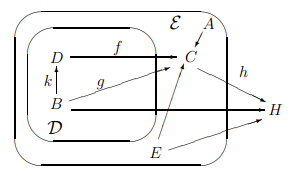
\includegraphics[scale=1]{1.png}
\end{center}
\end{multicols}
\subsection{Problema Arduo}
H è $\leq_F$-arduo per $\mathscr{E} \Leftrightarrow \forall A \in \mathscr{E}\:\:\:\: A \leq_F H$
\subsection{Problema Completo}
C è $\leq_F$-completo per $\mathscr{E} \Leftrightarrow C \leq_F$-arduo e $C \in \mathscr{E}$\\
Sia $\leq_F$ classifica $\mathscr{D}$ ed $\mathscr{E}$, allora C $\leq_F$-completo per $\mathscr{E}$, C $\subset \mathscr{D} \Leftrightarrow \mathscr{D} = \mathscr{E}$\\\\
Per ipotesi, $C \in \mathscr{D}, A \in \mathscr{E}$ allora $A \leq_F C$. Allora, per 3, anche $A \in \mathscr{D}$\\
Se $A \leq_F$-completo per $\mathscr{E}$, $B \in \mathscr{E}$ e $A \leq_F B \Leftrightarrow B \leq_F$-completo per $\mathscr{E}$. Quindi se un problema completo si riduce ad un altro problema della stessa classe, allora anche quest'altro problema è completo.\\
Questo perché $\forall D \in \mathscr{E} \Rightarrow D \leq_F A, A \leq_F B$ e per 2 $D \leq_F B$\\\\
Se $A \leq_F B$ allora, se la riduzione misura in qualche modo la difficoltà di un problema, $A$ \textbf{è al massimo difficile quanto} $B$ e $B$ \textbf{è più difficile (o uguale) di} $A$.\\
Quindi dovremmo cercare una famiglia di riduzioni che classificano $\mathscr{R}$ (ricorsive) e $\mathscr{RE}$ (ricorsive enumerabili).
\section{Classificare R ed RE}
Definiamo un insieme di funzioni $REC = \{\phi_x\:|\:\textsl{dom}(\phi_x) = N\}$ come l'\textbf{insieme di tutte le funzioni calcolabili}.
\begin{list}{}{}
	\item $TOT = \{x\:|\:\phi_x \in REC\}$
	\item $I \leq_{REC} J \Leftrightarrow \exists\: f \in REC$ $|$ $x \in I \Leftrightarrow f(x) \in J$
\end{list}
Per decidere la non appartenenza ad un insieme ricorsivamente enumerabile è necessario un \textbf{tempo infinito}.
\pagebreak
\paragraph{Th} La \textbf{relazione di riduzione} $\leq_{REC}$ classifica $\mathscr{R}$ e $\mathscr{RE}$
\subparagraph{Dim} Sappiamo che $\mathscr{R} \subseteq \mathscr{RE}$. Allora
\begin{enumerate}
	\item $id \in REC$, dalla definizione di $\mu$-ricorsiva
	\item $f$, $g \in REC \Rightarrow g(f) \in REC$ perché la composizione conserva la totalità
	\item $B \in \mathscr{R} \Rightarrow A = \{x \:|\: f(x) \in B\} \in \mathscr{R}$\\
	Per vedere se $A \in \mathscr{R}$ devo vedere se la funzione di $A$ è una funzione caratteristica calcolabile totale\\
	$\chi_A = \chi_B + f$ che è calcolabile totale perché $\chi_B$ è calcolabile totale
	\item \textbf{idem} per $\mathscr{RE}$ con la funzione semi-caratteristica di B, $\phi_i$ il cui dominino è $B$
\end{enumerate}
Il fatto che $\leq_{REC}$ classifichi $\mathscr{R}$ ed $\mathscr{RE}$ può essere visto come la capacità che hanno le funzioni calcolabili totali di \textbf{separare i problemi ricorsivi da quelli ricorsivamente enumerabili}: ciò avviene \textbf{in base al tempo necessario per decidere un problema}. Se il problema è \textbf{ricorsivo}, allora avremo la \textbf{risposta in tempo finito}, altrimenti il tempo necessario è infinito.\\
Inoltre, basta trovare un problema che sia $\leq_{REC}$-completo per $\mathscr{R}$ per poter vedere quali problemi sono decidibili e quali no.\\
Ancora più interessante è trovare un problema $\leq_{REC}$-completo per $\mathscr{RE}$: sapremmo quali sono i problemi \textit{al più} semi-decidibili e quale nemmeno semi-decidibili. Infatti basta ridurre il problema da studiare a quello completo e sapremo che è ricorsivamente enumerabile, oppure ridurre il problema completo a quello da studiare e sapremo che quest'ultimo, alla meglio, è ricorsivamente enumerabile.\\
Infatti è chiaro anche che $A \leq_{REC} B$, quindi
\begin{list}{}{}
	\item B è ricorsivamente enumerabile (B $\in \mathscr{RE}$) $\Rightarrow$ A $\in \mathscr{RE}$ (e forse A $\in \mathscr{R}$)
	\item A $\not\in\mathscr{RE} \Rightarrow$ B $\not\in\mathscr{RE}$ e sicuramente anche B $\not\in\mathscr{R}$
	\item Se A $\in\mathscr{R}$, il fatto che A $\leq_{REC}$ B non ci consente di dedurre niente sulla natura di B, che potrebbe essere ricorsivo o ricorsivamente enumerabile o nemmeno ricorsivamente enumerabile.\\
	Analogamente nel caso di A ricorsivamente enumerabile.
\end{list}
$K \leq_{REC} \overline{K}$? No. Perché $K \leq_{REC} \overline{K} \Leftrightarrow \overline{K} \leq_{REC} K$ e sarebbero entrambi $\mathscr{RE}$ ed è assurdo perché sappiamo che $K$ non è ricorsivo.
\paragraph{Oss} K è $\leq_{REC}$-completo per $\mathscr{RE}$, cioè K è $\mathscr{RE}$-completo
\subparagraph{Dim} $K \in \mathscr{RE}$ ok.\\
Dimostriamo che $\forall A \in \mathscr{RE} \Rightarrow A \leq_{REC} K$\\
Questo perché $A \rightarrow \exists\:\:\psi\: |\: A = \textsl{dom}(\phi_i)$ con $\psi$ calcolabile $\Rightarrow \exists\:\:\psi'$ calcolabile $|\: \psi'(x, y) = \psi(x)$\\
$A = \textsl{dom}(\psi) = \{x | \psi(x)\downarrow\} = \{x | \psi'(x, y)\downarrow\}$ e siccome è calcolabile allora ha indice: diciamo $i$\\
Quindi $A = \{x \: |\: \phi_i(x, y)\downarrow\} = \{x\: |\: \phi_{s(i, x)}(y)\downarrow\} = \{x\: |\: \phi_{s(i, x)}(s(i, x))\downarrow\}$ con $y = \lambda x.s(i, x)$ e perché $y$ non dipende da $\phi_{s(i, x)}$ e per il teorema del parametro.\\
Ottengo $\{x\:|\:s(i,x)\in K\}$ quindi $x\in A \Leftrightarrow f(x)\in K$ con $f(x) = \lambda x.s(i,x)$ che è totale, calcolabile e iniettiva perché lo è $s(i,x)$
\paragraph{Esercizio} $K \leq_{REC} TOT$?\\
Definisco $\psi(x, y)$ = 1 se x $\in$ K, indef altrimenti\\
La condizione $x \in K$ deve essere calcoalbile, così l'intera $\psi$ è calcolabile\\
$\psi$ calcolabile allora ha indice per C-T $\phi_i(x, y)$ ma se ha indice allora ho il teorema del parametro $\phi_{s(i, x)}(y)$ e posso usare la $f(x) = \lambda x.s(i, x)$ quindi
$$\phi_{f(x)}(y)$$
Vediamo i due casi
\begin{list}{}{}
	\item $x \in K$, $\forall y \psi(x, y) = 1 \Rightarrow \forall y \phi_{f(x)}(y) = 1 \Rightarrow f(x) \in TOT$ perché $\phi_{f(x)}(y)$ è calcolabile totale e $f(x)$ è indice
	\item $x \not\in K$, $\forall y \psi(x, y) =$ indef. $\Rightarrow \forall y \phi_{f(x)}(y) =$ indef. $\Rightarrow f(x) \not\in TOT$
\end{list}
I, $x \in I$, $\phi_y = \phi_x \Rightarrow y \in I$ insieme degli indici delle funzioni che calcolano la stessa funzione di $\phi_x$\\
I è un \textbf{insieme di indici che rappresentano le funzioni}. Caratterizzo le funzioni attraverso gli algoritmi che le calcolano.
\paragraph{Lemma} $A$ è un \textbf{insieme di indici che rappresentano funzioni} $A \neq \emptyset$ e $A \neq \mathbb{N}$\\$\Leftrightarrow$ $\forall$ $x$, $y$ ho $x \in A \wedge \phi_x = \phi_y \Rightarrow y \in A$ \\
$K \leq_{REC} A$ oppure (non esclusivo, possono essere vere entrambe) $K \leq_{REC} \overline{A}$
\subparagraph{Dim} $i_0$ sia l'indice della funzione ovunque indefinita $\phi_{i_0} = \lambda x.$indefinita\\
$i_0 \in A \vee i_0 \in \overline{A}$, sicuramente in uno dei due perché $A \neq \emptyset$ e $A \neq N$ quindi $\overline{A}$ "\textit{ha spazio}".\\
Sia $i_0 \in \overline{A}$, dimostro $K \leq_{REC} A$ (viceversa è una dimostrazione analoga) perché sia $i_1 \in A$ allora $\phi_{i_0} \neq \phi_{i_1}$\\
$\psi(x, y) = \left\{
\begin{array}{l c}
\phi_{i_1}(y) & \textsl{se }x \in K\\
\phi_{i_0}(y) & \textsl{altrimenti}
\end{array}\right.$
Calcolabile, per C-T ha indice: quindi, per il ragionamento precedente, $= \phi_{f(x)}(y)$
\begin{list}{}{}
	\item $x \in K$ allora $\phi_{f(x)}(y)  = \phi_{i_1}(y) \Rightarrow$ siccome $i_1 \in A$ insieme di indici che rappresentano funzioni e quindi $f(x) \in A$
	\item $x \not\in K$ allora $\phi_{f(x)}(y)  = \phi_{i_0}(y) \Rightarrow f(x) \in \overline{A} \Rightarrow f(x) \not\in A$
\end{list}
\paragraph{Lemma} $A$ è ricorsivo $\Leftrightarrow A = \emptyset \vee A = \mathbb{N}$

\section{Teorema di Rice}
"\textit{Con la sintassi si va poco lontano}."\\ %P. 70 delle note
Sia $\mathscr{A}$ un insieme di funzioni calcolabili.\\
L'insieme $A = \{x \:|\: \phi_x \in \mathscr{A}\}$ è \textbf{ricorsivo} $\Leftrightarrow$ $\mathscr{A} = \emptyset$ oppure $\mathscr{A}$ \textbf{contiene tutte le funzioni calcolabili}.
\paragraph{Dim} Corollario del lemma precedente. Si noti che $A$ è un'insieme di indici, mentre $\mathscr{A}$ è una classe di funzioni.\\
$A = \emptyset$ allora ok\\
$A = \mathbb{N}$ allora $\mathscr{A}$ rappresenta tutte le funzioni calcolabili quindi $A$ ricorsivo, altrimenti $K$ si riduce ad $A$ o $\overline{A}$ e si riduce alla dimostrazione di prima.\\
Si noti che $A$ è un insieme di indici, mentre $\mathscr{A}$ è una \textbf{classe di funzioni}: $A$ è \textbf{sintassi}, mentre $\mathscr{A}$ è \textbf{semantica}.
\paragraph{K non è un insieme di indici che rappresentano funzioni} Dimostriamolo.\\ Non deve valere $\forall\:x\in K\:\:\:\:\phi_x = \phi_y \Rightarrow y \in K$\\
Definiamo $\psi(x, y) = \left\{\begin{array}{l l}
	42 & \text{se }x = y\\
	\text{indefinita} & \text{altrimenti}
\end{array} \right.$\\Per C-T e per il teorema del parametro ho $\psi(x, y) = \phi_i(x, y) = \phi_{s(i,x)}(y) = \phi_{f(x)}(y)$\\
$\exists$ un punto fisso per $f(x) \Rightarrow \phi_{f(x)}(y) = \phi_x(y)$\\
Per $\psi(p,p) = \phi_p(p) = 42 \Rightarrow p\in K$\\
Per il padding lemma, $\exists$ un indice $z \neq p\:|\:\phi_z = \phi_p$\\
Però $\psi(p,q) = \phi_z(t) = \phi_p(z)$ è indefinita. Quindi $q\not\in K$ e $K$ non è un i.i.r.f.
\section{Considerazioni}
Questo risultato si ripercuote sulle proprietà che si possono dimostrare sui programmi: ogni metodo di prova si scontra con il problema della fermata. Ci sono però varie tecniche per aggirare il problema, ad esempio l'\textbf{analisi statica} del codice, dove si analizza il \textbf{testo} del programma, per raccogliere informazioni su come vengono usati durante l'esecuzione i vari oggetti (variabili, chiamate\ldots), per esempio se vengono rispettati i tipi, se si inizializzano\ldots\\
Si ha successo, con questo tipo di analisi, perché il \textbf{programma è approssimato in modo sicuro}: ciò che viene predetto è una sovra-approssimazione di ciò che succederà davvero. Per esempio, può succedere di dire che tra i valori assegnati ad una variabile \texttt{int} c'è una \texttt{String} senza che ciò accada a runtime, ma non capiterà mai di dire che tutti i valori assegnati sono \texttt{int} se a runtime a tale variabile viene assegnata una \texttt{String}.\\
A questa famiglia appartengono vari strumenti, spesso incorporati nei compilatori: type-checker, analizzatori data-flow e control-flow\ldots
\paragraph{Applicazione} Un'applicazione del teorema di Rice è che $K_1 = \{x\: |\: \textsl{dom}(\phi_x) \neq \emptyset\}$, cioè l'insieme degli indici delle funzioni definite in almeno un punto \textbf{non è ricorsivo}, sebbene sia ricorsivamente enumerabile.\\
Inoltre $K$, $K_0$ e $K_1$ si riducono l'un l'altro.
\begin{center}
Fine della Calcolabilità
\end{center}
\chapter{Complessità}
\paragraph{Fin'ora} Abbiamo studiato alcuni aspetti della teoria della calcolabilità: in particolare, abbiamo caratterizzato i \textbf{problemi risolubili} (rappresentati da funzioni calcolabili totali o da insiemi ricorsivi), quelli \textbf{insolubili} o \textbf{semi-decidibili} (rappresentati da funzioni calcolabili parziali o insiemi ricorsivamente enumerabili) e abbiamo discusso \textbf{problemi non decidibili} (rappresentati da funzioni non calcolabili o insiemi non ricorsivamente enumerabili.\\
Ora che abbiamo chiaro \textit{cosa} si può calcolare, ci si può porre il problema del \textit{come} calcolare. Sapendo distinguere il \textit{come} si calcola, riusciamo a distinguere tra loro le varie tecniche di calcolo, quindi a distinguere problemi \textit{facili} da \textit{difficili}. Primi passi verso una \textbf{teoria quantitativa} degli algoritmi.\\
Considereremo solo i problemi decidibili e di decisione ($x \in I$), cioè quei problemi o insiemi per cui esiste un algoritmo che ne calcoli la funzione caratteristica, e parleremo solamente delle risorse di tempo e spazio. Per vederle, modificheremo leggermente le MdT già viste trasformandole in \textbf{automi accettori}: cioè macchine che finiranno in uno stato di accettazione se l'ingresso appartiene all'insieme, altrimenti in uno stato di rifiuto.
\paragraph{Taglia} La \textbf{taglia} di un problema è il \textbf{numero di ingressi} della funzione, denotata con $|x|$
\paragraph{Valutare} Avere una $f$ funzione che \textbf{valuta asintoticamente l'utilizzo delle risorse}, cioè\\$f\:|\:f(|x|)\geq$ tempo/spazio. Studieremo la \textbf{complessità asintotica} al \textbf{caso pessimo}, per semplificazione.\\
Questa $f \geq$ determina una \textbf{classe di complessità}.\\
Le risorse si misurano in vari modi: numero di passi, nastri usati, numero di riduzioni fatte\ldots\\\\
Questa teoria è invariante rispetto al cambio di modello di calcolo ed alla rappresentazione dei dati.
\paragraph{Classi di gerarchia} Come si relazionano fra loro? Ce ne sono di particolarmente interessanti, caratterizzate da problemi particolarmente interessanti? Sicuramente abbiamo già sentito parlare della \textbf{classe di problemi risolvibili in tempo polinomiale deterministico P} e anche quella dei  \textbf{problemi risolvibili in tempo polinomiale non deterministico NP}, che sono due classi particolarmente interessanti cercando la loro relazione e le loro proprietà.
$$\mathscr{RE} \supset \mathscr{R} \supset \textsl{NPSPACE} = \textsl{PSPACE} \supseteq \mathscr{NP} \supseteq \mathscr{P} \supseteq \textsl{Logspace}$$
\begin{list}{}{Considerando}
	\item \textsl{Logspace}: insieme delle funzioni il cui tempo di calcolo è asintoticamente simile al logaritmo della taglia
	\item \textsl{NPSPACE} e \textsl{PSPACE} uguali, ma diversi da \textsl{Logspace}
	\item Non esiste ancora una dimostrazione di $\mathscr{P} \subseteq \mathscr{NP}$
	\item Per decidere la non appartenenza ad $\mathscr{R}$ basta un tempo finito, ma per decidere la non appartenenza a $\mathscr{RE}$ no.
\end{list}
\paragraph{Problema completo} Data una famiglia di riduzioni F che classifica due classi $\mathscr{D}$ ed $\mathscr{E}$, un problema $I$ è $\leq_F$-completo per $\mathscr{D}$ (analogo per $\mathscr{E}$) $\Leftrightarrow$ $\forall\:J\in\mathscr{D}\:J\leq_F I$
\paragraph{Tesi di Cook-Karp} $\mathscr{P}$ è la \textbf{classe dei problemi trattabili} mentre $\mathscr{NP}$ è la \textbf{classe dei problemi intrattabili}
\paragraph{} Bisogna ora decidere \textit{come} si misuro lo spazio o il tempo necessario per decidere $x \in I$.
\pagebreak
\section{Misure di complessità deterministiche}
\paragraph{MdT a $k$ nastri} MdT come tutte le altre (Q, $\Sigma$, $\delta$, q$_0$)\\
La funzione di transizione $\delta$ è un po' diversa e $h$, stato di terminazione, viene diviso in 2: stato \textbf{si} (stato di accettazione) e stato \textbf{no} (stato di rifiuto), entrambi $\not\in$ Q. Operano in \textbf{modo sincrono su $k$ nastri}.\\\\
Per ciascun simbolo, $\delta$ dovrà fornire il nuovo simbolo e spostare sincronamente le testine quindi fornire una direzione: 
$\delta(q, \sigma_1, \sigma_2, \ldots, \sigma_k) = (q', (\sigma'_1, D_1), (\sigma'_2, D_2), \ldots, (\sigma'_k, D_k))$\\
La configurazione iniziale sarà leggermente diversa, quindi: 
$\gamma = (q_0, u_1 \sigma_1 v_1, u_2 \sigma_2 v_2, \ldots, u_k \sigma_k v_k)$\\
Una transizione d'esempio: $(q, u_1\sigma_1 v_1, u_2\sigma_2 v_2, \ldots, u_k \sigma_k v_k) \rightarrow (q', u'_1\sigma'_1 v'_1, u'_2\sigma'_2 v'_2, \ldots, u'_k \sigma'_k v'_k)$\\$\delta$ : $Q\times\Sigma^k \longrightarrow Q\cup\{\textsc{si}, \textsc{no}\}\times(\Sigma\times\{\textsc{l}, \textsc{r}, -\})^k$
\paragraph{Tempo} Il tempo di richiesto da $M$ a $k$ nastri per decidere $x \in I$ è $t \Leftrightarrow$ partendo dallo stato iniziale $q_0$ ho $(q_0, \underline{\triangleright}x, \underline{\triangleright}, \ldots, \underline{\triangleright}) \longrightarrow_M^t (H, w_1, \ldots, w_k)$ con $H \in \{$si, no$\}$\\
Non si può sempre decidere il numero esatto di passi, ci accontenteremo di una \textbf{stima superiore} $f(|x|)$, con $|x| =$ taglia$(x)$. Non sapremo come calcolare la taglia in generale, ma deve essere relativamente \textbf{facile} farlo: lunghezza di un vettore, dimensione in memoria\ldots\\
$M$ \textbf{decide} $I$ in tempo $f \Leftrightarrow \forall\: x$ il tempo $t$ per decidere $x \in I$ è tale che $t \leq f(|x|)$
\subparagraph{TIME($f$)} $= \{I\:|\: \exists\: M$ che decide $I$ in tempo deterministico $f\}$\\\\
$O(f) = \{g\:|\:\exists\: r \in R$ per cui $g(n) < r\cdot f(n)\}$ salvo un pezzo iniziale. Cioè la $f$ da un certo punto in poi sta sopra la $g$.\\$\Omega(f)$ è quando la $f$ sta sotto.\\$\Theta(f)$ è quando le funzioni crescono allo stesso modo.
\subsection{Teorema di Riduzione del Numero di Nastri}
\paragraph{Teorema} Teorema che dimostra che usando una macchina parallela si "guadagna" tempo in modo quadratico.\\
$\forall\:M$ a $k$ nastri che decide I in $O(f)$ deterministica $\Rightarrow\exists\:M'$ a 1 nastro che decide $I$ in $O(f^2)$
\paragraph{Dim}: Costruisco $M'$ per simulare $M$.

\begin{enumerate}
	\item Da $_k\gamma$ di $M$ (cioè a $k$ nastri), simulo ogni configurazione in di $M$\\$(q, \triangleright u_1 \sigma_1 v_1, \triangleright u_2 \sigma_2 v_2, \ldots, \triangleright u_k \sigma_k v_k)$ con quelle di $M'$ così fatte $(q', \triangleright \triangleright' u_1 \overline{\sigma_1} v_1 \triangleleft' \triangleright' u_2 \overline{\sigma_2} v_2 \triangleleft'\ldots \triangleright' u_k \overline{\sigma_k} v_k \triangleleft')$ usando le "parentesi $\triangleright'$ e $\triangleleft'$ per separare i $k$ nastri sul nastro singolo e usando \#$\Sigma$ nuovi simboli $\overline{\sigma_i}$ per ricordare la posizione su ogni nastro.
	\item Sistemare il nastro iniziale generando la configurazione iniziale di M: $(q_0,\underline{\triangleright} \triangleright' x \triangleleft' \triangleright' \triangleleft' \ldots \triangleright' \triangleleft' )$\\Bastano $2k + \#\Sigma$ nuovi stati: si trova il primo \#, si torna indietro cambiando stato e si codifica il simbolo $\neq$ \# che c'è, sostituirlo con \#, spostarsi a destra scrivendo il simbolo ricordato. Ripetere gli ultimi due passi per $|x| - 1$ volte, mentre andare fino al primo \# richiede $|x| + 1$ passi e un nuovo stato. Ora si scrive $\triangleright'$ sulla casella \# corrente, si torna sulla prima vuota muovendosi a destra scrivendo $k-1$ coppie $\triangleright'\triangleleft'$ usando altri $2\cdot(k-1)$ stati.
	\item Per simulare una mossa di $M$, $M'$ scorre il nastro da sinistra a destra per scovare i caratteri correnti, quelli sovralineati: avanti e indietro una volta.\\
	Riscorro il nastro per scrivere i nuovi simboli e fissare i nuovi correnti: avanti e indietro seconda volta (con una cascata di spostamenti a destra se bisogna spostare un $\triangleleft'$ a destra.
	\item Infine quando $M$ si ferma, si ferma anche $M'$ eventualmente rimuovendo le "parentesi" $\triangleright' \triangleleft'$ e sostituendo i $\overline{\sigma_i}$ con i corrispondenti $\sigma_i$
\end{enumerate}
Ricordando che \textbf{non si può usare più spazio che tempo}, cioè non si possono vedere più caselle di quanti passi si fanno, per simulare un passo ci vogliono al massimo 4$K$ passi.\\
Il nastro contiene al massimo $K = k\cdot (2 + f(|x|)) + 1$ con $|x|$ = taglia$(x)$, con $+2$ per le parentesi $\triangleright' \triangleleft'$ e $+1$ per $\triangleright$\\\\
$M$ fa $f(|x|)$ passi, $M'$ fa $f(|x|) \cdot 4K$ quindi $f(|x|) \cdot \not k \cdot (\not 2 + f(|x|)) + \not 1)$ con la roba cancellata perché non dipende dall'input ma dalla macchina.\\
Quindi $M$ fa $O(f)$ mentre $M'$ fa $O(f^2)$
\paragraph{Conseguenze} Miglioramenti accettabili "algoritmicamente", come aggiungere nastri o processori che operino in parallelo, non cambiano le funzioni calcolate e non modificano il tempo richiesto se non polinomialmente: le MdT sono stabili anche rispetto alla testi di Cook-Karp.
\subsection{Teorema di Accelerazione Lineare}
\paragraph{Teorema} Se $I \in$ TIME$(f(n))$ $\Rightarrow$ $\forall\: \epsilon \in R^+$ si ha $I\in$ TIME$(\epsilon\cdot f(n) + n + 2)$
\subparagraph{Dim} Intuizione su come determinare $\epsilon$:  \textbf{condensare un certo numero di caratteri in un carattere unico}\\
	$\sigma_1 \sigma_2 \ldots \sigma_m \longrightarrow [\sigma_1 \sigma_2 \ldots \sigma_m]$, con $[\sigma_1 \sigma_2 \ldots \sigma_m]$ \textbf{unico carattere}.\\
	Stati codificati in una tripla $[q, \sigma_1 \sigma_2 \ldots \sigma_m, k]$ con $k$ che indica la posizione del cursore.\\
	Equivale ad avere macchine con parole di dimensioni crescenti, $2^m$ bit.\\\\
$M'$ in 6 passi simula $m$ passi di $M$, con $M'$ macchina veloce e $M$ macchina lenta, questo perché partizionando l'input in blocchi di $m$ caratteri i cambiamenti possono essere fatti in blocchi contigui. Nei primi 4 passi $M'$ fa a sinistra, poi a destra, poi ancora a destra e poi ritorna sul carattere corrente $s = [\sigma_1\sigma_2\ldots\sigma_m]$ per raccogliere i simboli che $M$ potrebbe visitare e codificarli nep proprio stato. Quando $M$ compie $m$ mosse, $M'$ le simula muovendosi a sinistra, o a destra, del simbolo corrente $s$, comunque modificando solo due simboli incluso $s$ (le altre 2 mosse).\\
$M'$ farà $|x|+2$ passi per condensare l'input + $6\cdot \lceil \frac{f(|x|)}{m} \rceil$ passi, quindi posso prendere come $m = \lceil \frac{6}{\epsilon} \rceil$
\paragraph{Risultati} Quindi se ho un algoritmo che decide un problema in tempo deterministico $f(n)$, allora l'algoritmo $\in$ TIME$(f(n))$ e posso costruirne un altro che lo calcola in tempo deterministico $\epsilon f(n) + n + 2$, questo per ogni $\epsilon$: posso accelerare l'algoritmo \textbf{linearmente} quanto voglio.\\
Quindi se $f = c\cdot n$ posso eliminare $c$ e mettere $\epsilon = \frac{1}{c}$, se $f = c_1n^k + \ldots + c_{k-1}n + c_k$ posso rendere $c_1 = 1$ e ignorare gli addendi con esponenti minori di $k$ perché vengono dominati da $n$ sufficientemente grande, giustificando l'uso di $O(n^k)$.\\
Questo teorema \textbf{consente di usare gli ordini di grandezza per approssimare} senza \textit{fare niente di male}. Inoltre si possono eliminare le costanti (dipendenti dalle macchine su cui si calcola) perché macchine più potenti tendono a farle rimpicciolire e valori grandi di $|x| = n$ tendono a ridurre l'\textit{importanza} delle costanti.
\paragraph{} Grazie a questi risultati definisco $\mathscr{P}$, la classe dei problemi decidibili in tempo polinomiale deterministico, come $$\mathscr{P} = \bigcup_{k \geq 1} \textsl{TIME}(|x|^k) $$
\paragraph{Ricapitolando}
\subparagraph{} M richiede tempo $t$ per decidere $I$ $\Leftrightarrow$ $M(x) = (q_0, \triangleright x, \triangleright, \ldots, \triangleright) \rightarrow^t (h, w_1, \ldots, w_k)$ con $h \in \{\textsl{si, no}\}$
\subparagraph{} M decide $I$ in tempo $f$ $\Leftrightarrow$ $\forall\:x\in I\:\:M(x) \rightarrow^t (\textsl{si}, w_1, \ldots, w_k)$ cioè M richiede tempo $t$ per deciderlo, con $t \leq f(|x|)$
\subparagraph{TIME($f$)} $=\{I\:|\:\exists\: M$ che decide $I$ in tempo $f\}$\\
$\mathscr{P} = \bigcup_{k \geq 1} \textsl{TIME}(|n|^k)$
\subparagraph{}Abbiamo anche scoperto che \textbf{non si può usare più spazio che tempo}.
\paragraph{Spazio necessario al calcolo} Quantità di celle che il programma utilizza durante l'esecuzione.\\
Ignoreremo lo spazio utilizzato dal nastro d'ingresso.
\section{MdT I/O a $k$ nastri}
Si tratta di una MdT in cui il \textbf{primo nastro contiene l'ingresso} mentre l'\textbf{ultimo nastro contiene l'uscita}.
$$\delta(\sigma_1, \ldots, \sigma_k) = (q', (\sigma_1', D_1), \ldots, (\sigma_k', D_k))$$
\paragraph{Nastro d'ingresso} Ogni $\delta$ come sopra deve essere tale che il primo nastro ($\sigma_1', D_1$) sia di \textbf{sola lettura} perché è il nastro dell'input.\\
La \textbf{condizione} quindi è che $\sigma'_1 = \sigma_1$ \textbf{sempre}, cioè \textbf{il nastro di ingresso è di sola lettura}.
\paragraph{Nastro d'uscita} Analogamente ci deve essere una condizione sul nastro d'uscita:
\begin{list}{}{}
	\item $D_k = R$
	\item oppure $D_k = -\Rightarrow\sigma_k' = \sigma_k$, cioè \textbf{nastro d'uscita di sola scrittura}.
\end{list}
\paragraph{Altra condizione} Inoltre, bisogna costruire le $\delta$ in modo che quando finisco di leggere il nastro d'ingresso, finendo quindi sul carattere bianco $\#$, io debba necessariamente tornare indietro. Altrimenti, anche se non scrivo niente, potrei usare le operazioni di spostamento sui caratteri bianchi per codificare delle operazioni. Quindi \begin{list}{}{}
	\item $\sigma_1 = \# \Rightarrow D_1 \in \{\textsl{L}, -\}$
\end{list}
\paragraph{Teorema} Collega le MdT a $k$ nastri con le MdT di tipo I/O a $k+2$ nastri\\$\forall\:M$ a $k$ nastri che decide $I$ in tempo deterministico $f\Rightarrow\exists\:M'$ a $k+2$ nastri $I/O$ che decide $I$ in tempo $c\cdot f$\\
La dimostrazione, intuitivamente, consiste per $M'$ nel copiare il nastro d'ingresso sul secondo nastro e, a computazione conclusa ed eseguita come $M$, copiare il nastro d'uscita sull'ultimo nastro.
\subsection{Complessità in spazio}
\paragraph{} $M$ a $k$ nastri di tipo I/O che va $(q_0, \triangleright x, \triangleright, \ldots, \triangleright) \rightarrow^t (h, w_1, \ldots, w_k)$ con $h \in \{\textsl{si, no}\}$ richiederà, come spazio, quello dei nastri di lavoro $w_i$. Hanno spazio costante, quindi so in principio qual'è. Quindi:
\begin{list}{}{}
	\item $M$ a $k$ nastri I/O richiede spazio $\sum_{i=2}^{k-1} |w_i| \Leftrightarrow (q_0, \triangleright x, \triangleright, \ldots, \triangleright) \rightarrow^t (h, w_1, \ldots, w_k)$
\end{list}
Questo perché il numero delle celle usate dai nastri non diminuisce mai: nel primo nastro perché è di sola lettura, nell'ultimo perché è di sola scrittura e nei $k-2$ nastri di lavoro perché i caratteri bianchi a destra non scompaiono mai.\\\\
Ad esempio, per $k = 3$ avrò un unico nastro di lavoro, quindi lo spazio occupato dalla macchina sarà quello del nastro di lavoro (come detto prima, ignoriamo l'occupazione in spazio dei nastri input e output).
\paragraph{$M$} decide $I$ in spazio $f \Leftrightarrow \forall\: x\:\:M$ richiede spazio $\leq f(|x|)$
\paragraph{SPACE($f$)} = $\{I\: |\:\exists\: M$ che decide $I$ in spazio $f\}$
\paragraph{} Ignoriamo lo spazio occupato dai nastri di input e output perché altrimenti avremmo complessità in spazio almeno lineari: questo perché il nastro in input misura sempre $|x| + 1$ contenendo $\triangleright x$, mentre il nastro in output contiene un "bit", un segnale per accettare o rifiutare, nel caso dei problemi $I$ di decisione considerati, quindi non rilevante nelle misure.\\
Esistendo classi interessanti e importanti che sono sub-lineari nello spazio, come visti successivamente, ci interessano misure più fini.
\paragraph{Teorema} Posso ridurre linearmente lo spazio.\\
$I \in$ SPACE$(f) \Rightarrow \forall\:\epsilon\in R^+\:\: I \in$ SPACE$(2 + \epsilon\cdot f(n))$
$$\textsl{PSPACE} = \bigcup_{k\geq 1} \textsl{SPACE}(n^k)$$
$$\textsl{LogSPACE} = \bigcup_{k\geq 1} \textsl{SPACE}(k\cdot\log(n))$$
Come per $\mathscr{P}$, anche queste classi sono invarianti rispetto al modello di calcolo usato.\\
Abbiamo inoltre che $\textsl{LogSPACE}\subsetneq\textsl{PSPACE}$
\pagebreak
\paragraph{Teorema} $\textsl{LogSPACE} \subseteq \mathscr{P}$
\subparagraph{Dim} Sia $I \in \textsl{LogSPACE} \Rightarrow \exists\: M$ di tipo I/O che $\forall\:x\in I$ decide $x$ in spazio $O(\log|x|)$\\
Quante \textbf{configurazioni diverse posso avere sul nastro di lavoro}? Dipende da quanti simboli ho sulla macchina. Poniamo $x$ input e la sua lunghezza $|x| = n$, avrò $\#\Sigma^{\log(n)}$ nastri diversi, cioè il numero di simboli (cardinalità di $\Sigma$) alla $\log (n)$. Inoltre posso avere il cursore in $\log(n)$ posizioni diverse in ciascun stato (che sono $\# Q$). Inoltre il cursore sta anche nell'input, in $|x|$ posizioni diverse. Quindi le configurazioni diverse del nastro di lavoro sono 
$$n\cdot\log(n)\cdot\# Q\cdot\#\Sigma^{\log(n)}$$
Per dimostrare che $\textsl{LogSPACE} \subseteq \mathscr{P}$ devo trovare $k$ tale che $n\cdot\log(n)\cdot\# Q\cdot\#\Sigma^{\log(n)} \leq n^k$. Applico il $\log$ da entrambi i membri
$$\log(n) + \log(\log(n)) + \log(\# Q) + \log(n)\log(\#\Sigma) \leq k\cdot\log(n)$$
Elimino $\log(\log(n))$ perché è molto piccolo, e $\log(\# Q)$ perché è una costante, poi semplifico per $\log(n)$
$$\not\log(n) + \not\log(n)\log(\#\Sigma) \leq k\cdot\not\log(n)$$
$$1 + \log(\#\Sigma) \leq k$$
Quindi basta usare $k \geq \log(\#\Sigma)$.\\\\
Come conseguenza, scopriamo che \textbf{lo spazio limita il tempo}, perché se passo troppe volte sopra la solita configurazione vado in ciclo.
\paragraph{Ricapitolando} MdT a $k$ nastri, eventualmente di tipo I/O. $\forall\:x$ macchina $M(x) \rightarrow^t M$ in una situazione di alt.
Riesce perché: \textbf{aggiungere nastri}, \textbf{avere I/O}, \textbf{aumentare la parola} su cui lavorano le macchine (quindi \textbf{compattare} simboli) sono tutte \textbf{operazioni algoritmicamente effettive}: si possono fare con algoritmi. Ciò fornisce un bel vantaggio.\\
Però sorge un \textbf{problema}: dobbiamo decidere un insieme (quindi risolvere un problema) che \textbf{sappiamo essere decidibile} e calcolare una funzione che \textbf{sappiamo essere calcolabile}, ma non riusciamo a individuare una struttura matematica e delle proprietà tramite le quali risolverlo \textit{facilmente}.\\
Per esempio per costruire una macchina che decideva se una data stringa fosse palindroma, \textbf{abbiamo sfruttato una proprietà} delle stringa: che essa sia leggibile da destra a sinistra e da sinistra a destra. In questo caso era banale, ma ci sono problemi per cui non conosciamo la struttura e ciò rende la vita difficile.
\subsection{Spazio degli stati}
\begin{list}{}{Lo spazio degli stati di una MdT può essere}
	\item \textbf{Generato esplicitamente}, 
	\item \textbf{Generato implicitamente}, guess \& try
\end{list}
\section{MdT non deterministica}
N = (Q, $\Sigma$, $\Delta$, $q_0$) \textbf{MdT non deterministica}
\begin{list}{}{}
	\item \textbf{Relazione di transizione} $\Delta \subseteq (Q\times\Sigma)\times(Q\times\{\textsl{si, no}\}\times\Sigma\times\{Q, L, -\})$\\
	Possono essere presenti più quintuple associate allo stesso stato ed allo stesso simbolo, quindi molte configurazioni $(q', u'\sigma'v')$ raggiungibili da $(q, u\sigma v)$ in un solo passo
	\item \textbf{Stato iniziale} $\gamma = (q, u\sigma v) \rightarrow (q', u'\sigma'v')$
	\item \textbf{Computazione} $M(x) \rightarrow\gamma_1\rightarrow\ldots\rightarrow\gamma_n$ cioè $M(x) \rightarrow^n\gamma_n$, un \textbf{cammino} (non un albero!)
\end{list}
La potenza del non determinismo si vede nel modo in cui si accetta: \textbf{basta che ci sia un cammino che porti alla soluzione} perché il problema sia risolto.
\pagebreak
\paragraph{DNA Computing} Calcolo eseguito ricombinando fra loro sequenze biologiche invece che per passi come da tradizione.
\paragraph{Come decide un problema una macchina non deterministica} Di seguito la definizione.\\
N decide I $\Leftrightarrow$ $\forall\: x \in I \Rightarrow \exists$ computazione $M(x) \rightarrow^* (\textsl{si, }w)$\\
Se $x \in I$ allora e solamente allora deve esistere \textit{almeno una} computazione, un cammino, che accetta $x$.\\
Il contrario è che \textbf{tutte rifiutino}, allora $x \not\in I$\\
\begin{center}
	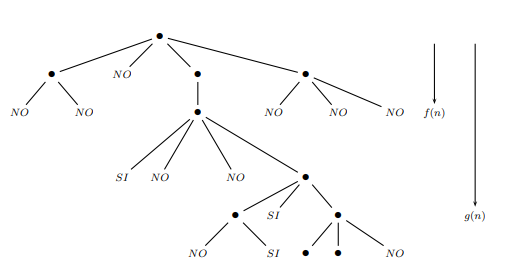
\includegraphics[scale=1]{grafo_nondet.png}
\end{center}
Numerando gli archi di decisione identifico una computazione tramite la successione di numeri. Data una certa $\sigma$ ho tante quintuple in $\Delta$, le enumero e le ordino in qualche modo. Prendo la $n_1$ scelta dallo stato iniziale, la $n_2$ scelta dallo stato risultante\ldots\\
Nell'esempio, una scelta Si è identificata dalla computazione $(2, 0, 0)$, un'altra da $(2, 0, 3, 1)$.
\subsection{Misure di complessità non deterministica}
\paragraph{Tempo} $N$ MdT non deterministica decide $I$ in \textbf{tempo non deterministico} $f(|x|)$ (più semplicemente $f$) $\Leftrightarrow$
\begin{list}{}{}
	\item $N$ decide $I$, e
	\item $\forall\: x \in I\:\:\:\exists\: t\:|\:N(x)\rightarrow^t(\textsl{si, }w) \wedge t \leq f(|x|)$
\end{list}
$\textsl{NTIME}(f) = \{I \:|\:\exists\:N$ che decide $I$ in tempo non deterministico $f\}$\\
Quindi una MdT non deterministica accetta $x$ in tempo non deterministico $f$ se e solo se c'è \textbf{almeno} una computazione che termina in \textit{si} in $t \leq f(|x|)$ passi. Invece, non accetta $x$ se \textbf{tutte} le sue computazioni lunghe al massimo $f(|x|)$ terminano in \textit{no}.\\
C'è nuovamente asimmetria: non basta che per un elemento $x\not\in I$ ci sia una computazione che porta in \textit{no} in meno di $f(|x|)+1$ passi, ma devono farlo \textbf{tutte}. L'asimmetria tra il decidere $I$ e $\overline{I}$ è rafforzata dal richiedere che ciò venga svolto in tempo $f(|x|)$.\\
Questo perché \textbf{affinché $N$ decida $I$ basta che per \textit{ogni} $x$ ci sia \textit{almeno una} computazione che lo accetta}.
$$\mathscr{NP} = \bigcup_{k\geq 1}\textsl{NTIME}(n^k)$$
Abbiamo che $\mathscr{P}\subseteq\mathscr{NP}$ dato che ogni MdT deterministica è anche non deterministica.
\pagebreak
\paragraph{Teorema} Se $I \in \textsl{NTIME}(f) \Rightarrow I \in \textsl{TIME}(c^f)   $ con $c \geq 1$ che \textbf{dipende soltanto dalla macchina} in $\textsl{TIME}(f)$.\\ In altre parole: se $I$ è deciso da $N$ a $k$ nastri in tempo non deterministico $f(x)$, allora $\exists\:M$ a $k+1$ nastri che decide $I$ in $O(c^{f(x)})$, $c \geq 1$ che dipende solo da $N$\\
In altre parole $\textsl{NTIME}(f) \subseteq \textsl{TIME}(c^f)$
\subparagraph{Dim} Il grado di diramazione massimo, o il \textbf{grado di non determinismo}, è 
\begin{list}{}{}
	\item $d = \textsl{max}\{\textsl{grado}(q, \sigma)\:|\:q\in Q, \sigma \in \Sigma\}$
	\item dove $\textsl{grado}(q, \sigma) = \#\{(q', \sigma', D)\:|\:((q, \sigma), (q', \sigma', D))\in \Delta \}$
\end{list}
Per ogni stato $q \in Q$ e ogni simbolo $\sigma \in \Sigma$ ordino totalmente, ottenendo così che ogni computazione è una sequenza di scelte lunga $t$, indicabili come una sequenza di $t$ numeri naturali nell'intervallo $[0\ldots d-1]$. Una macchina $M$ che simula $N$ produce una successione di scelte partendo sempre dal principio. Per esempio riproduce la scelta 20300 e magari arriva in uno stato di accettazione. Se ci arriva, bene \textbf{ho finito}.\\
Se non ci arriva prende il prossimo numero $t+1$ in base $d$, nell'esempio 20301.\\
Se supera il numero di archi la stringa aumenta di un carattere e faccio 00, 01, 02\ldots poi 10, 11, 12\ldots\\
Il numero delle successioni da visitare sarà dell'ordine di $d^{f(n)}$ con $c = d$.\\
Ho una perdita esponenziale. Ma aggiungere il non determinismo non cambia le classi dei problemi.
\paragraph{Spazio} $N$ decide $I$ in \textbf{spazio non deterministico} $f(|x|)$ (più semplicemente $f$) $\Leftrightarrow$
\begin{list}{}{}
	\item $N$ decide $I$, e
	\item $\forall\: x \in I\:\:\:\exists\:w_1,\ldots, w_k\:|\:(q_0, \underline{\triangleright}x,\ldots,\underline{\triangleright})\rightarrow_N^*($Si$, w_1, \ldots, w_k)$ e $\mathlarger{\sum_{2\leq i \leq k-1}|w_i| \leq f(|x|)}$
\end{list}
$\textsl{NSPACE}(f) = \{I\:|\:\:\exists\:N$ che decide $I$ in spazio non deterministico $f$\}\\
$\textsl{NPSPACE} = \bigcup_{k\geq 1}\textsl{NSPACE}(n^k)$
\paragraph{Teorema di Savitch} $\textsl{NPSPACE} = \textsl{PSPACE}$
$$\textsl{LogSpace} \subseteq \mathscr{P} \subseteq \mathscr{NP} \subseteq \textsl{PSPACE} + \textsl{NPSPACE} \subset \mathscr{R} \subset \mathscr{RE}$$
$$\mathscr{P} ? \mathscr{NP}$$
\paragraph{} Siamo giunti alla conclusione che una MdT non deterministica accetta $x$ in tempo $f$ $\Leftrightarrow$ $\forall\:x\in I$ $\exists$ una computazione $N(x)\rightarrow^t($Si$, w)$ con $t \leq f(|x|)$\\
Per confutare invece, bisogna che \textbf{tutte} le computazioni rifiutano, cioè per rifiutare $x$ bisogna che $\forall$ computazione $N(x) \rightarrow^t ($No$, w)$ con $t \leq f(|x|)$
\subsection{Commesso Viaggiatore}
$n$ città connesse da strade, la distanza fra la città $i$ e la città $j$ è $d(i,j)$. Sulle distanze vale la proprietà riflessiva e la diseguaglianza triangolare.\\
Le distanze sono rappresentate con le coppie $(i, j)$ che sono $O\left(\mathlarger{\frac{n\cdot(n-1)}{2}}\right)$. Il problema è trovare un cammino che tocchi le città una ed una sola volta, con costo minimo. Il costo è la somma delle distanze percorse.\\
Cerchiamo quindi una \textbf{permutazione} degli indici $i, j$ in modo tale che la somma delle distanze sia minima. Una permutazione è una bigezione $\Pi : \left[1, n\right] \rightarrow \left[1, n\right]$.\\
Il nostro costo $\mathlarger{\sum_{1\leq i \leq n-1} d(i, i+1)} \leq B$ con $\Pi(h) = i$ e $\Pi(k) = i+1$, cioè $i$ e $i+1$ sono permutazioni di, rispettivamente, un certo $h$ ed un certo $k$.
\paragraph{Forza Bruta} Deterministica
\begin{enumerate}
	\item \textbf{Generare l'intero spazio di ricerca}, cioè tutte le possibile permutazioni esistenti $\Pi$ come stringhe, che sono nell'ordine di $n! = O(n!)$
	\item \textbf{Certificazione}: prendere la prima permutazione e verificare se è $\leq B$.\\
	$n$ accessi al nastro d'ingresso, uno per città, e $n^2$ per vedere la distanza di ciascuna città, quindi $O(n\cdot n^2)$
\end{enumerate}
Esponenziale in tempo ma lineare $O(n)$ in spazio, perché si mantiene una singola permutazione alla volta.\\
Dire che non esiste soluzione richiede di valutare tutte le permutazioni.
\paragraph{MdT non deterministica}
\begin{enumerate}
	\item Bisogna \textbf{scrivere una MdT non deterministica} che generi ad ogni passo un numero tra $1$ ed $n$ compresi: abbiamo così una permutazione delle città.\\Con un po' di accorgimenti si evitano stringhe del tipo $111\ldots$, ad esempio scrivendo la MdT in modo che non rigeneri numeri già generati.
	\item \textbf{Certificazione}: la stringa è una permutazione $\Pi$? Si scopre in $n$ passi.\\
	Dopodiché faccio esattamente la certificazione precedente, per verificare se $\leq B$: tutto ciò si fa in $O(n^3)$ come prima.
\end{enumerate}
\section{Funzioni di valutazione}
Una \textbf{funzione di valutazione} potrebbe essere una qualunque funzione calcolabile che dalla dimensione dell'input porti in un numero naturale che indica la valutazione: numero di passi, di moltiplicazioni\ldots\\
Sappiamo che le classi di complessità formano una gerarchia: ad esempio la classe $\textsl{TIME}(O(n^3))$ cioè i problemi risolvibili in tempo cubico, include propriamente quelli risolvibili in tempo quadratico. Questo lo sappiamo dall'esperienza. Perché queste funzioni funzionino dobbiamo porre loro dei vincoli: chiameremo queste funzioni\\\textbf{appropriate}/oneste/costruibili.\\
\begin{list}{}{Vincoli:}
	\item \textbf{Monotone crescenti}\\
	Significa che se devo risolvere un problema la cui dimensione è maggiore di un altro problema ci devo mettere più tempo che spazio.
	\item $\exists\:M\:|\:\forall\:x\in\Sigma^*$ si arresta (dando come risultato $\diamond^{f(|x|)}$, $\diamond \not\in \Sigma$ carattere speciale, lungo tanti caratteri quanto $f(|x|)$) in tempo $O(f(|x|) + |x|)$ con l'addendo $|x|$ per rendere lineare quando $f(|x|)$ è sub-lineare e spazio $O(f(|x|))$
\end{list}
Esempi: $n^k, \lfloor\log n\rfloor, n!, k^n,\ldots$\\
Se $f$, $g$ sono appropriate, anche $f(g)$, $f^g$, $f\cdot g$, $f + g$\ldots: la classe è chiusa per una serie di operazioni.
\subsection{Teorema di gerarchia}
Data $f$ appropriata, allora (ricordando che $\textsl{TIME}(f(n))=\{I\:|\:\exists\:M$ che decide $I$ in tempo $f(n)\}$)
\begin{list}{}{}
	\item $\textsl{TIME}(f(n))\subsetneq\textsl{TIME}(f(2n + 1)^3)$
	\item $\textsl{SPACE}(f(n))\subsetneq\textsl{SPACE}(f(n)\cdot\log(f(n)))$
\end{list}
La dimostrazione è omessa, si noti che quella del primo punto si basa sulla dimostrazione che il problema\\$\{x\:|\:\phi_x(x)$ termina in $f(|x|)$ passi$\}$, che è un pezzetto di $K$, appartiene a $\textsl{TIME}(f(2n+1)^3)$ ma non a $\textsl{TIME}(f(n))$\\
Analogamente per le MdT non deterministiche.
\paragraph{} Possiamo ora dimostrare la nostra gerarchia, in particolare che $\mathscr{P} \subsetneq \textsl{EXP} = \mathlarger{\bigcup_{k \geq 1}\textsl{TIME}(2^{n^k})}$
\subparagraph{Dim} Sappiamo che $\mathscr{P} \subseteq \textsl{EXP}$, cioè $\mathscr{P} \subseteq \textsl{TIME}(2^n)$ perché al crescere di $n$ per qualunque $k$, $n^k \leq 2^n$\\
Abbiamo quindi $\mathscr{P} \subseteq \textsl{TIME}(2^n) \subsetneq\textsl{TIME}(f(2^{(2n + 1)^3})) \subseteq \mathlarger{\bigcup_{k \geq 1}\textsl{TIME}(2^{n^k})}$
\subsection{Qualche assioma}
\begin{list}{-}{}
	\item $\textsl{SPACE}(f(n))\subseteq\textsl{NSPACE}(f(n))$
	\item $\textsl{TIME}(f(n))\subseteq\textsl{NTIME}(f(n))$
	\item $\textsl{NSPACE}(f(n))\subseteq\textsl{TIME}(k^{\log n + f(n)})$
\end{list}
Avevamo anche dimostrato che $\textsl{NTIME}(f(n)) \subseteq \textsl{TIME}(c^{f(n))}$ da cui deriva $\mathscr{NP} \subseteq \textsl{EXP}$\\
Si ricorda quindi anche che
$$\textsl{LogSpace} \subseteq \mathscr{P} \subseteq \mathscr{NP} \subseteq \textsl{EXP}$$
\pagebreak
\paragraph{}Abbiamo dei motivi per cui non possiamo fare a meno delle funzioni di misura appropriate.
\subsection{Teorema} \textbf{Troveremo sempre problemi via via più difficili}, cioè la gerarchia non è superiormente limitata.\\
$\forall\:g$ calcolabile totale $\exists\:I$ problema$\:|\:I\in\textsl{TIME}(f(n))\wedge I\not\in\textsl{TIME}(g(n))$, con $f > g$ quasi ovunque\\
Quindi la gerarchia tratta dal teorema di gerarchia continua a crescere senza fermarsi mai.\\
Con \textit{quasi ovunque} si intende \textbf{dappertutto eccetto che in un numero finito di punti}.
\subsection{Teorema di Accelerazione (Blum)} Il teorema di accelerazione \textit{lineare} diceva che possiamo accelerare \textit{linearmente} la soluzione del problema.\\
Blum ci dice che \textbf{non sempre esiste un algoritmo ottimo} per un problema.\\\\
$\forall\:h$ calcolabile totale\\
$\exists\:I\:|\:\forall\:M$ che decide $I$ in tempo $f\:\:\exists\:M'$ che decide $I$ in tempo $f'\:|\:f(n)>h(f'(n))$ quasi ovunque\\\\
$h$ indica quanto è più veloce $M'$ rispetto a $M$\\
\textbf{Intuitivamente}: supponendo di avere una macchina universale lenta, e di ottenere una macchina universale nuova e velocissima, allora avremmo dei programmi che rimangono più veloci sulla macchina vecchia che non sulla nuova.\\
In altre parole, si può dimostrare l'esistenza di una successione di algoritmi via via più efficienti per risolvere il problema costruito in funzione di $h$. Si sa solo che esiste, ma non come costruirla.
\subsection{Teorema della Lacuna (Borodin)}
$\exists\:f$ calcolabile totale $|\:\textsl{TIME}(f) = \textsl{TIME}(2^f)$\\
\textbf{Intuitivamente}: c'è un insieme di programmi che sono altrettanto efficienti/veloci su una macchina lenta che su una macchina nuova.\\
Questo cozza con un risultato del teorema di gerarchia, che arrivava a dire (a grandi linee)\\$\textsl{TIME}(f(n)) \subsetneq \textsl{TIME}(f(2n + 1)^3)$ perché avrei $\textsl{TIME}(f^2) = \textsl{TIME}(f) \subsetneq \textsl{TIME}(f^3)$, ma quindi avrei una situazione assurda del tipo $A = B < C$, come può essere $A = C$? Ma il teorema di gerarchia vale. Ciò che cambia è che nel teorema della lacuna $f$ non è richiesta appropriata. Questo ci dice che \textbf{non possiamo fare a meno delle funzioni di misura appropriate}, o di classi di funzioni con vincoli a come misuriamo il consumo delle risorse in modo che il teorema di gerarchia valga.
\subsection{Teoria della Complessità Astratta}
Si svincola dal tipo di risorsa misurata e dal modello di calcolo.\\
Una funzione $\phi$ è una misura di complessità se restituisce un numero naturale avendo come ingressi una funzione $\psi$ e $x$ parametro di $\psi$. Inoltre soddisfa entrambi i seguenti assioni: \begin{list}{}{}
	\item $\phi(\psi, x)$ è definita (converge) $\Leftrightarrow \psi(x)$ è definita (converge)\\
	Questo assioma ci dice che $\phi$ misura la complessità del calcolo di $\psi(x)$.
	\item $\forall\:\psi, x, k$ è decidibile se $\phi(\psi, x) = k$\\
	Questo assioma assicura che si può davvero misurare la complessità del calcolo di $\psi(x)$.
\end{list}
Quindi se $\phi$ misurasse il numero di passi, riotterremmo la definizione di complessità in tempo, mentre se misurasse il numero di celle riotterremmo quella in spazio.
\subsection{Tesi di Cook-Karp}
\begin{list}{-}{}
	\item $\mathscr{P}$ sono i problemi \textbf{trattabili}
	\item $\mathscr{NP}$ sono i problemi \textbf{intrattabili}
\end{list}
Nel senso che avendo un algoritmo che funziona in tempo polinomiale ($\mathscr{P}$), allora il problema può essere risolto "efficientemente", altrimenti se il problema sta in $\mathscr{NP}$ allora è troppo difficile per essere gestito da un programma.\\\\
Sono \textbf{robuste}, cioè resistono al cambio di modello. Ponendo $M$, $M'$ \textbf{modelli di calcolo} (quindi MdT, \texttt{while}-calcolabili\ldots), allora posso passare da $M \longrightarrow M'$ mediante un polinomio.\\
Inoltre $\mathscr{P}$ e $\mathscr{NP}$ sono chiusi rispetto alle classiche operazioni ma anche alle riduzioni in sottoclassi dei polinomi. Significa che se riduco il problema $I \leq_F J$, con $F \subseteq$ polinomi e $I\in\mathscr{C} \Rightarrow f(I) = J \in\mathscr{C}$\\\\
Ci sono algoritmi esponenziali al caso pessimo, ma efficientissimi nei casi più comuni: ad esempio l'algoritmo del simplesso, la paginazione, l'inferenza dei tipi in ML\ldots\\
Ma non sempre posso sapere qual è il caso medio di un problema.
\subsection{Riduzione efficiente}
$I$ si riduce efficientemente a $J \Leftrightarrow (x\in I \Leftrightarrow f(x)\in J$ con $f \in \textsl{logspace})$ e si può scrivere $I \leq J$\\
Otteniamo che $\leq$ classificano $\textsl{logspace}$ e una qualunque classe $\mathscr{E} \in \{\mathscr{P}, \mathscr{NP}, \textsl{EXP}, \textsl{PSPACE}, \textsl{NPSPACE}\}$\\
Se prendo una $\mathscr{D} \subseteq \mathscr{E}$, allora $\leq$ classificano $\mathscr{D}$ ed $\mathscr{E}$ (quindi ad esempio $\mathscr{P}$ ed $\mathscr{NP}$)\\
Dato che $\textsl{logspace}\leq\mathscr{P} \Rightarrow \leq_\mathscr{P}$ classificano $\mathscr{D}$ ed $\mathscr{E}$. Lo si dimostra così, tramite le proprietà della classificazione di una famiglia di riduzioni:
\begin{enumerate}
	\item $\textsl{id} \in \textsl{logspace}$, banalmente
	\item $f, g \in \textsl{logspace} \Rightarrow f(g)\in \textsl{logspace}$\\
	$f \in \textsl{logspace} \Rightarrow \exists\:M$ che opera in $\textsl{logspace}$, analogamente per la $g$ avrò $M'$. La nuova macchina può considerare l'ultimo nastro di $M$ come nastro di lavoro di $M'$ e calcolare così la composizione delle due. Questa nuova macchina sta in $\textsl{logspace}$? Se prendo ad esempio $f = \textsl{id}$ ho input e output lungo $n$, e la somma dei nastri di lavoro è $n$, quindi lineare e non logaritmica. Allora si fa partire $M'$ in modo da richiedere a $M$ i dati di lavoro e usarli all'occorrenza sostituendoli sempre su una sola casella. Otteniamo così il $\textsl{logspace}$
	\item $I\leq J$, $J \in \mathscr{D} \Rightarrow I \in \mathscr{D}$\\
	Se $I$ si riduce per un logaritmo a $J$, e $J$ lo risolvo in tempo logaritmico allora risolvo in tempo logaritmico anche $I$
	\item $I\leq J$, $J \in \mathscr{E} \Rightarrow I \in \mathscr{E}$\\
	Analogo al punto precedente.
\end{enumerate}
Quindi $\leq_{\textsl{logspace}}$ \textbf{sono riduzioni efficienti} e \textbf{classificano} $\mathscr{P}$ ed $\mathscr{NP}$\\
Una delle conseguenze è che se trovo un problema completo dentro $\mathscr{P}$ (cioè che tutti i problemi di $\mathscr{P}$ si riducono a lui e lui $\in\mathscr{P}$) allora in qualche modo ho rappresentato la difficoltà massima e $\mathscr{P}$ non ha problemi più difficili perché tutti i problemi si riducono a lui.\\
Poiché riesco a trovare soluzioni tra problemi in $\mathscr{P}$, questo vuol dire che le soluzioni di tutti i problemi all'interno di una classe hanno una struttura matematicamente analoga tra loro.
\section{Richiami di logica}
Ponendo $x_1,\ldots,x_n \in X$ \textbf{variabili} e la \textbf{grammatica} $$B\longrightarrow tt\:|\:ff\:|\:x\:|\:\neg B\:|\:B_1 \vee B_2\:|\:B_1 \wedge B_2$$ con $tt$, $ff$, $x$ e $\neg x$ chiamati \textbf{letterali} $l_1,\ldots$.\\
Diciamo che $V : X' \longrightarrow \{T, F\}$ con $X' \subset X$ è un \textbf{assegnamento booleano}.\\
B è \textbf{chiusa} se \textbf{non ha variabili}. Un assegnamento booleano è \textbf{buono} se \textbf{lega tutte le variabili di B}.
\paragraph{Soddisfacibilità} Cioè quando un assegnamento booleano rende vera un'espressione booleana.\begin{list}{}{}
	\item $V \vDash tt$ banalmente
	\item $V \vDash x$ quando $V(x) = tt$
	\item $V \vDash \neg B$ quando $V \not\vDash B$
	\item $V \vDash B_1 \vee B_2$ quando $V \vDash B_1$ oppure $V \vDash B_2$
	\item $V \vDash B_1 \wedge B_2$ quando $V \vDash B_1$ e $V \vDash B_2$
\end{list}
\paragraph{Forma normale} $B$ è in \textbf{forma normale congiuntiva} $\Leftrightarrow$ $B = \mathlarger{\bigwedge_{i=1}^n C_i}$ e $C_i = \mathlarger{\bigvee_{j=1}^m l_j}$ con $l_j$ letterali\\
$B$ è in \textbf{forma normale disgiuntiva} $\Leftrightarrow$ $B = \mathlarger{\bigvee_{i=1}^n C_i}$ e $C_i = \mathlarger{\bigwedge_{j=1}^m l_j}$ con $l_j$ letterali\\
Inoltre $\forall\:B\:\:\exists\:B'$ in forma normale (una delle due) $|\:(V\vDash B \Leftrightarrow V\vDash B')$.\\
Questo si ottiene avendo, da $B$ con $O(n)$ simboli, un $B'$ con $O(2^n)$ simboli.\\\\
\textbf{Considereremo espressioni solo in forma normale congiuntiva}.
\section{Alcuni problemi}
\subsection{Problema SAT}
Anche chiamato \textbf{problema della soddisfacibilità}. La formulazione è semplice:
$$\text{Dato }B\text{, allora }\exists\:V\:|\:V\vDash B\text{ ?}$$
SAT $\in\mathscr{NP}$. Come faccio a dirlo? Dovrei costruire una macchina non deterministica che verifica questa cosa, cioè che dice se l'assegnamento esiste o meno. Come si fa?\\
Cominciando dallo stato iniziale. Supponendo $n$ variabili, allora ho $n$ scelte all'inizio, per ognuna delle quale ho due scelte: assegnare $tt$ o assegnare $ff$. Lo faccio per la prima, due scelte, poi per la seconda\ldots facendo così tutti i possibili assegnamenti. \textbf{Un cammino è un assegnamento}.\\
Vedremo invece che la verifica se un assegnamento soddisfa possiamo farla dinamicamente, quindi è \textbf{polinomiale} perché è nel numero delle variabili.
\subsection{Problema HAM}
Problema del cammino hamiltoniano. Dato un grafo orientato $G = (N, A)$, $\exists?$ cammino che tocca tutti i nodi una ed una sola volta?\\
Vediamo che $\text{HAM} \leq \text{SAT}$. Devo definire $f \in \textsl{logspace}\:|\:$ ($G$ ha un cammino hamiltoniano $\Leftrightarrow f(G) = B$ è tale che $\exists\:V\vDash B$)\\
Vedremo una riduzione, ma non è la migliore.\\\\
Supponiamo che $G = (N, A)$ ha $n$ nodi (cioè l'insieme $\{1, 2, \ldots, n\}$), allora $B$ ha $n^2$ variabili $x_{i,j}$: ciascuna rappresenta che nell'$i$-esimo posto di un cammino appare il nodo $j$. Posso rappresentarle anche come $(i, j)$ con $i, j \in [1, n]$.\\
Definiamo una permutazione $\Pi : [1, n] \rightarrow [1, n]\:|\:\left(\Pi(i), \Pi(i+1)\right) \in A$, dai nodi ai nodi. In realtà nella nostra permutazione, i primi sono i nodi mentre i secondi sono le posizioni che occupano nel cammino. con $\Pi(i)$ rappresento il nodo in posizione $i$.\\
$\Pi$ deve essere davvero una funzione:
\begin{enumerate}
	\item Un nodo non può essere mappato due volte. Quindi: $\neg(x_{ij} \wedge x_{kj})$ con $i \neq k$. Questo però non è un congiunto, quindi applico DeMorgan\\
	$\Longrightarrow \neg x_{ij} \vee \neg x_{kj}$ con $i \neq k$
	\item La funzione deve essere definita ovunque (totale), quindi ogni nodo deve apparire nel cammino.\\
	$\Longrightarrow x_{1i} \vee x_{2i} \vee \ldots \vee x_{ni}$
	\item[] Ho definito che la funzione è totale, quindi ora devo definire la sua surgettività.
	\item Ogni posizione deve ricevere un nodo, sennò rimane un pezzo "vuoto".\\
	$\Longrightarrow x_{i1} \vee x_{i2} \vee \ldots \vee x_{in}$
	\item Non posso avere due nodi nella solita posizione. Quindi: $\neg(x_{ij} \wedge x_{ik})$ con $j \neq k$. Applico DeMorgan.\\
	$\Longrightarrow \neg x_{ij} \vee \neg x_{ik}$ con $j \neq k$
	\item[] Ho ben definito la permutazione $\Pi$, quindi ora se riesco a prendere tutti i disgiunti, metterli in and e trovo un assegnamento booleano che li rende veri ho trovato un cammino hamiltoniano. Manca da definire $\left(\Pi(i), \Pi(i+1)\right) \in A$
	\item Se $(i, j) \not\in A \Longrightarrow \neg x_{k,i} \vee \neg x_{k+1, j}$
\end{enumerate}
Adesso devo dimostrare che se c'è un cammino hamiltoniano allora esiste un assegnamento che soddisfa. Dimostro i due versi dell'implicazione separatamente:
\begin{list}{}{}
	\item[$\Leftarrow$] $\forall\:j\:\:\exists!\:i\:|\:V(x_{ij}) = tt$, così definiamo la valutazione. Cioè per ogni posizione del cammino $i$ c'è un solo nodo $j$, quindi solo un $x_{ij}$ è vera per ogni $i$.\\
	Nello stesso modo $\forall\:i\:\:\exists!\:j\:|\:V(x_{ij}) = tt$, cioè ogni nodo $j$ è in una sola posizione del cammino, quindi una sola $i$ per cui $x_{ij}$ è vera.\\
	Grazie anche alla 5, che garantisce che ci sia il cammino, ho definito la $V$
	\item[$\Rightarrow$] Ho un cammino, composto da $(\Pi(1), \Pi(2), \ldots, \Pi(n))$, quindi definisco la $V(x_{ij}) = \left\{\begin{array}{l}
	tt\:\:\text{ se }\Pi(j) = i\\
	ff\:\:\text{ se }\Pi(j) \neq i
\end{array}	 \right.$
\end{list}
Finito. Ho definito una permutazione che rispetta il fatto che gli archi siano ben rappresentati.\\Manca di dimostrare che $f \in \textsl{logspace}$.
\paragraph{} Dobbiamo costruire una macchina di tipo I/O, così sappiamo misurare lo spazio necessario (somma dello spazio usato dai nastri di lavoro). Naturalmente l'alfabeto della nostra macchina conterrà: simboli di verità, connettivi logici, parentesi, e due caratteri 0 e 1. Perché gli indici delle variabili sono rappresentati in binario.\\
L'input è la successione degli archi. La macchina scrive in binario il numero di nodi $n$ sul nastro di lavoro. Poi avrò tre ulteriori nastri di lavoro, poiché nelle formule 1|5 compaiono 3 indici: un nastro per $i$, uno per $j$ e uno per $k$.\\
Per scorrere le clausole farà scorrere da 1 a $n$ gli indici sui nastri di lavoro. Quando ha scritto le quattro formule 1|4, comincia a scrivere sull'output l'ultima formula, la 5. Scorrerà il nastro input anche questa volta per verificare la clausola, finendo ad un certo punto.\\
Perché è in $\textsl{logspace}$? $\mathlarger{\sum_{i=2}^5} |w_i|$, ma $i$ arriva fino ad $n$ che rappresentato in binario richiede $\log n$. Quindi abbiamo 5 nastri di $\log n$, quindi $\mathlarger{\sum_{i=2}^5} |w_i| = 5\log n$ cioè $f\in \textsl{SPACE}(5\cdot\log n)$
\paragraph{} Da un \textbf{problema nel mondo dei grafi} ho ottenuto \textbf{la sua soluzione mediante la soluzione di un problema di deduzione logica}. Abbiamo \textbf{ricondotto un problema sui grafi ad un problema di logica}.\\
Diventa esplicita la \textbf{struttura comune} fra i due problemi.
\subsection{Problema CRICCA}
Un problema risolto positivamente se in un certo grafo non orientato esiste un sottoinsieme dei nodi detto \textbf{cricca} tale per cui, per ogni coppia di nodi all'interno della cricca c'è un arco che li congiunge.\\
Formalmente: dato $G = (N, A)\:\:\exists?\:C\subseteq N\:\:|\:\:\forall\:i,j\in C\:(i,j)\in A$.\\
$C$, cioè la cricca, è di ordine $k$ se contiene $k$ nodi.\\
Vediamo come SAT $\leq$ CRICCA, cioè \textbf{riconduciamo un problema di logica ad uno sui grafi}.\\\\
$\exists\:V\vDash B = \mathlarger{\bigwedge_{i=1}^n} C_i \Leftrightarrow f(B) = (N, A)$ ha $n$-cricca.\\Otteniamo che
\begin{list}{}{}
	\item $N$ è l'insieme delle occorrenze dei letterali $l$ in $B$
	\item $A = \{(i, j)\:|\: i\in C_k \Rightarrow (j\not\in C_k \wedge i \neq \neg j)\}$ cioè metto un arco tra due nodi solo se non sono all'interno dello stesso letterale né se sono uno il negato dell'altro.
\end{list}
Da questo ottengo che se c'è una cricca c'è un assegnamento booleano, viceversa se c'è un assegnamento booleano c'è una cricca, quindi è una riduzione.\\
Appartiene a $\textsl{logspace}$ perché posso usare lo stesso meccanismo della rappresentazione binaria e mantenendo gli indici sui nastri di lavoro.
\pagebreak
\subsubsection*{Funzioni Booleane}
$$V \vDash B \Leftrightarrow f(V(x_1), \ldots, V(x_n)) = tt\:\:\: f: X \rightarrow \{0, 1\}$$
$f$ si \textbf{costruisce mediante un circuito booleano}, cioè un grafo $G = (N, A)$ \textbf{aciclico}, con 
\begin{list}{}{}
	\item $i \in N$ nodi\\
	\textbf{Sorta} $s(i) = \{tt, ff, \neg, \wedge, \vee\} \bigcup X$ ($X$ variabili)\\
	\textbf{Ingressi} le porte con $s(i) \subset \{tt, ff\} \bigcup X$\\
	\textbf{Uscita} $i$ la porta più in alto (il massimo del circuito quando viene ordinato con ordinamento parziale)\\
	Se $s(i) = \neg \Rightarrow i$ ha 1 ingresso ed 1 uscita\\
	Se $s(i) \subset \{\wedge, \vee\} \Rightarrow i$ ha 2 ingressi e 1 uscita\\
	Per calcolare l'uscita ho bisogno di una funzione di valutazione che assegni i valori di verità agli ingressi, definiamone la semantica
	\begin{multicols}{2} \begin{list}{}{}
		\item $[i]_V = tt$ se $s(i) = tt$
		\item $[i]_V = f$ se $s(i) = ff$
		\item $[i]_V = V(x)$ se $s(i) = x$
		\item $[i]_V = \textsl{not}([j]_V)$ se $(j, i) \in A$ e $s(i) = \neg$
		\item $[i]_V = [j]_V \textsl{ and } [h]_B$ se $(j, i), (h, i) \in A$ e $s(i) = \wedge$
		\item $[i]_V = [j]_V \textsl{ or } [h]_B$ se $(j, i), (h, i) \in A$ e $s(i) = \vee$
	\end{list} \end{multicols}
	\item $(i, j) \in A$
\end{list}
\paragraph{Esempio} $(x \vee (x \wedge y)) \vee ((x \wedge y) \wedge \neg(y \vee z))$
\subsection{Circuit SAT}
$$\exists\:V\:\:|\:\:[C]_V = tt ?$$ con $[C]_V = [n]_V$ con $n$ porta di uscita. Questo problema $\in \mathscr{NP}$\\
\textbf{Circuit Value}: se $C$ non ha variabili, $[C]_\emptyset = tt$? Questo è il problema della soddisfacibilità, per verificare se dato un assegnamento il circuito è soddisfatto o meno.\\
\textbf{Circuit Value} $\in \mathscr{P}$, perché tengo sul nastro input la rappresentazione del grafo, cioè l'insieme delle coppie che formano gli archi e la sorta di ogni nodo (porta). Sui nastri di lavoro tengo i valori dei vari livelli di porte, ma non ho ripetizioni quindi è polinomiale: non bisogna farsi confondere dal fatto che il numero totale delle porte può essere esponenziale rispetto alla profondità del circuito (cioè al livello della porta d'uscita), perché la taglia del circuito è data dal numero $n$ di porte.\\\\
Notiamo che \textbf{Circuit Value $\leq$ Circuit SAT}, perché SAT è la versione più generale di Value.\\Value è la versione di SAT in cui non ho bisogno della funzione di assegnamento.\\\\
Più interessante è scoprire che Circuit SAT $\leq_{\textsl{logspace}}$ SAT. Intuitivamente è vero, costruiamo la riduzione.\\
Significa che $\forall$ circuito con variabili $\in X$, dobbiamo trovare una $f \in \textsl{logspace}\:\:|\:\:[C]_V = tt \Leftrightarrow\exists\:V'\supseteq V\:\:\:V'\vDash f(C)$\\
$V(x) = tt \Rightarrow V'(x) = tt$ e $f(C) = \bigwedge B_k$\\
Le variabili di $f(C)$ includono tutte le variabili di $C$, cioè $X$, unito ad una variabile per ogni porta,\\cioè $X \cup \{x_i = i\:|\:i \in N\}$
\begin{list}{}{}
	\item Se $g$ è la porta di uscita $\Rightarrow$ genera un congiunto $g$ variabile
	\item Se $s(i) = tt$ o $ff$ $\Rightarrow$ genera un congiunto $i$ nel primo caso, $\neg i$ nel secondo caso
	\item Se $s(i) = x \Rightarrow (i \Leftrightarrow x)$ cioè $i$ è vero se e soltanto se $x$ è vero, cioè $(i \Rightarrow x) \wedge (x \Rightarrow i)$ cioè $(\neg i \vee x) \wedge (\neg x \vee i)$
	\item Se $s(i) = \wedge \Rightarrow (i$ è vero$ \Leftrightarrow h \wedge k)$ con  $(h,i), (k,i)\in A$ , espandendola diventa $\neg(i \vee h) \wedge (\neg i \vee k) \wedge (\neg h \vee \neg k \vee i)$
	\item Se $s(i) = \vee \Rightarrow (i$ è vero$ \Leftrightarrow h \vee k)$ con  $(h,i), (k,i)\in A$ , espandendola diventa $(\neg i \vee h \vee k) \wedge (\neg h \vee i) \wedge (\neg k \vee i)$
\end{list}
\pagebreak
\paragraph{} Usando $x \wedge ff$ come esempio, mettendo come nodi $h = x$, $g = \wedge$ e $k = ff$, ottengo la formula $$g \wedge \neg k \wedge (\neg h \vee x) \wedge (h \wedge \neg x) \wedge(\neg g \vee h) \wedge (\neg g \vee k) \wedge (\neg h \vee \neg k \vee g)$$
 Vediamo che $[g] = ff\:\:\forall\:V$
\begin{list}{}{}
	\item $g \wedge$ $\longrightarrow V(g) = tt$ 
	\item $\neg k \wedge$ $\longrightarrow V(k) = ff$
	\item $(\neg h \vee x) \wedge$ 
	\item $(h \wedge \neg x) \wedge$
	\item $(\neg g \vee h) \wedge$
	\item $(\neg g \vee k) \wedge$ $\longrightarrow V(k) = tt$ ottenendo un assurdo
	\item $(\neg h \vee \neg k \vee g)$
\end{list}
\section{Tabella di computazione}
Prendiamo un problema $I \in \mathscr{P} \Leftrightarrow \exists\:M\:\:|\:\:\forall\:x \in I M(x)\longrightarrow_t ($si/no, $w)$ con $t \leq |x|^k$\\
Ho la configurazione iniziale $\underline{\triangleright}a_1\ldots a_n$, copo un certo passo ho $\triangleright\underline{a_1}\ldots a_n$ e così via.\\
Posso immaginare di mettere il tutto in una matrice:$\begin{array}{c c c c}
\underline{\triangleright} &a_1&\ldots & a_n\\
\triangleright&\underline{a_1}&\ldots& a_n\\
\triangleright\\
\triangleright\\
\end{array}$\\
Ad ogni riga $i$ ho il passo di computazione e la configurazione al passo $i$: ho rappresentato l'intera computazione in una matrice. Possiamo dare a questa \textbf{tabella di computazione} un \textbf{formato standard}.
\paragraph{Tabella di computazione} Una matrice quadrata $T[i, j]$ con $1 \leq i,j \leq |x|^k$ se $M(x)$ termina in $|x|^k - 2$ passi. \textbf{Condizioni}:
\begin{enumerate}
	\item La macchina termina in meno di $|x|^k - 2$ passi, come detto
	\item Presa la riga $i$, essa comincia con il respingente e termina con tutti i caratteri bianchi.\\
	Tutte le caselle non significative di una riga, quindi, sono riempite con $\#$\\
	Siccoma la lunghezza della riga è $|x|^k$, ma la macchina termina in $|x|^k - 2$ passi, non avrò mai il cursore in ultima posizione perché il tempo limita lo spazio.
	\item Supponiamo il cursore in una posizione, posso codificare lo stato nell'alfabeto\\
	L'alfabeto contiene $\sigma_q \in (\Sigma \times Q \times \{h\})$ che registra che nella configurazione $i$-esima il cursore si trova nella posizione $j$, si legge $\sigma$ e lo stato è $q$. Basta prendere $\Sigma \times Q$ nuovi simboli.
	\item All'inizio il cursore è sul primo carattere subito dopo il respingente. In più i passaggi sul respingente "indietro-avanti", cioè i due passi obbligati successivi di andare sul respingente e tornare a destra, vengono condensati in un singolo passo. Così facendo, il cursore non si troverà mai sul respingente. C'è un'eccezione, nel caso seguente
	\item Quando $T[i, j] =$ si/no, allora sposta il cursore fino alla seconda colonna (con massimo $O(|x|^k)$ passi), introducendo uno stato ausiliario di finto arresto. Lo stato di accettazione, se raggiunto, è quindi sempre in $T(l, 2)$ per qualche $l \leq |x|^k$.\\
	Si ammette che il cursore passi sopra il simbolo $\triangleright$ quando lo stato sia $q_{SI}$ (abbreviazione di $\sigma_{q_{SI}}$), con il vincolo che non debba mai toccare il $\triangleright$ più a sinistra (che rappresenta l'inizio del nastro).
	\item Se $\sigma_{SI}$ oppure $\sigma_{NO}$ appaiono sulla riga $p<|x|^k$ e nella seconda colonna, allora tutte le righe di indice $q$ con $p\leq q \leq |x|^k$ sono uguali alla $p$-esima
\end{enumerate}
Abbiamo l'ovvia condizione di terminazione con successo: M accetta $x$ $\Leftrightarrow \exists\:i\:\:|\:\:T(i, 2) = \sigma_{SI} (= T(|x|^k, 2))$\\
Su una tabella di computazione T di una macchina di Turing $M$ che decide $I$ in $|x|^k$, con $x$ lungo $n$ caratteri, ho una serie di fatti:
\begin{list}{}{}
	\item $T(1, 2)$ contiene lo stato iniziale e il primo carattere di $x$ $x_q^1$\\
	Inoltre $\forall\:j, 2\leq j \leq |x| + 1$, la casella $T(1, j)$ contiene il $j - 1$-esimo simbolo di $x$\\
	Infine, $\forall\:j, |x| + 2 \leq j \leq |x|^k$, la casella $T(1, j)$ contiene $\#$
	\item $\forall\:i, T(i, 1) = \triangleright$
	\item $\forall\:i, T(i, |x|^k) = \#$ (si impiega meno spazio che tempo!)
	\item $T(i, j) = $ come determinarlo? (Osservazione tratta dall'esempio successivo)\\
	L'elemento $T(i, j)$ dipende dall'elemento $T(i-1, j\pm1)$ oppure da $T(i-1, j)$. Nell'esempio successivo, $T(4, 4)$ dipende da $T(3, 4)$, $T(8, 3)$ da $T(7, 4)$ e $T(11, 5)$ da $T(10, 4)$\\
	\textbf{Ciascuna cella}, quindi, \textbf{dipende solo e solamente dalle tre precedenti}. Questo perché ad ogni passo la macchina si sposta di un posto solo.\\
	Quindi $T(i, j)$ dipende solo da $T(i-1, j-1)$, $T(i-1, j)$, $T(i-1, j+1)$ e dalla $\delta$.
\end{list}
Una tabella di computazione, quadrata, ha $|x|^k$ righe/colonne. Siccome si ferma in $|x|^k - 2$ passi, abbiamo la sicurezza che la prima colonna è composta da tutti $\triangleright$ e l'ultima è composta da tutti $\#$ perché non si può usare più spazio che tempo.\\
La prima riga, oltre il respingente, avrà i caratteri $x_1\:x_2\:\ldots\:x^n$ e dopo tutti caratteri bianchi $\#$. Le righe rappresentano i passi di computazione, fino a che ad un certo punto (in una certa riga = un certo passo di computazione) in un certo carattere si troverà uno stato di accettazione $\sigma_h$. Questo stato di accettazione viene portato, nei passi successivi, in seconda posizione (subito dopo il respingente) e da quella riga in poi sono tutte uguali, per cui l'ultima riga sarà $\triangleright\:\sigma'_h\:\ldots\:\#$
\paragraph{Esempio} MdT che verifica se una stringa è palindroma. Esempio: la stringa \texttt{abba}, 16 passi per verificare, quindi 18 righe e colonne
\begin{center}
\begin{math}
	\begin{array}{r l l l l l l l l l l}
		 & 1 & 2 & 3 & 4 & 5 & 6 & 7 & \ldots & 17 & 18\\
		\hline
		1 & \triangleright & a_{q_0} & b & b & a & \# & \# & \ldots & \# & \#\\
		2 & \triangleright & \triangleright & b_{q_A} & b & a & \# & \# & \ldots & \# & \#\\
		3 & \triangleright & \triangleright & b & b_{q_A} & a & \# & \# & \ldots & \# & \#\\
		4 & \triangleright & \triangleright & b & b & a_{q_A} & \# & \# & \ldots & \# & \#\\
		5 & \triangleright & \triangleright & b & b & a & \#_{q_A} & \# & \ldots & \# & \#\\
		6 & \triangleright & \triangleright & b & b & a_{q'_A} & \# & \# & \ldots & \# & \#\\
		7 & \triangleright & \triangleright & b & b_{q_1} & \# & \# & \# & \ldots & \# & \#\\
		8 & \triangleright & \triangleright & b_{q_1} & b & \# & \# & \# & \ldots & \# & \#\\
		9 & \triangleright & \triangleright & b_{q_0} & b & \# & \# & \# & \ldots & \# & \#\\
		10 & \triangleright & \triangleright & \triangleright & b_{q_B} & \# & \# & \# & \ldots & \# & \#\\
		11 & \triangleright & \triangleright & \triangleright & b & \#_{q_B} & \# & \# & \ldots & \# & \#\\
		12 & \triangleright & \triangleright & \triangleright & b_{q'_B} & \# & \# & \# & \ldots & \# & \#\\
		13 & \triangleright & \triangleright & \triangleright & \#_{q_0} & \# & \# & \# & \ldots & \# & \#\\
		14 & \triangleright & \triangleright & \triangleright_{SI} & \# & \# & \# & \# & \ldots & \# & \#\\
		15 & \triangleright & \triangleright_{SI} & \triangleright & \# & \# & \# & \# & \ldots & \# & \#\\
		16 & \triangleright & \triangleright_{SI} & \triangleright & \# & \# & \# & \# & \ldots & \# & \#\\
		17 & \triangleright & \triangleright_{SI} & \triangleright & \# & \# & \# & \# & \ldots & \# & \#\\
		18 & \triangleright & \triangleright_{SI} & \triangleright & \# & \# & \# & \# & \ldots & \# & \#\\
	\end{array}
\end{math}
\end{center}
\subsection{Circuit Value è $\mathscr{P}$-completo}
$\forall\:I\in\mathscr{P}$, $x \in I \Leftrightarrow [f(x)]_\emptyset = tt$ con $f \in \textsl{logspace}$\\
$I\in\mathscr{P} \Rightarrow \exists\:M$ che decide $x$ in $|x|^k = n^k \Rightarrow M(x) \rightarrow^t ($SI, $w)$ con $t \leq n^k - 2$\\
Allora \textbf{costruiamo la tabella di computazione}, aggiungendo ad $M$ $\Sigma \times Q \cup \{h\}$ nuovi simboli. Chiamo $\Sigma'$ il nuovo alfabeto.\\
Ciascun simbolo $\rho \in \Sigma'$ viene mappato in una stringa di bit, successioni di 0/1 $(s_1,\ldots,s_m)\in\{tt, ff\}^m$, con\\$m = \lceil\log_2(\#\Sigma')\rceil$ cioè numero di bit necessari per rappresentare i $\#\Sigma'$ simboli contenuti in $\Sigma'$.\\
Posso codificare il respingente e il carattere bianco come preferisco, ad esempio $\triangleright = tt\ldots tt$ e $\# = ff\ldots ff$\\
Ogni elemento della tabella quindi diventa una sequenza di $m$ bit: $T(i, j) = s_{i,j,1}, s_{i,j,2},\ldots,s_{i,j,m}$, cioè $m$ simboli ciascuno che codifica anche la riga $i$ e la colonna $j$.\\
$T(i,j) = f\left( \begin{array}{l l l l}
	s_{i-1,j-1,2}, & s_{i-1,j-1,2}, &\ldots, &s_{i-1,j-1,m},\\
	s_{i-1,j,2}, &s_{i-1,j,2}, &\ldots, &s_{i-1,j,m},\\
	s_{i-1,j+1,2}, &s_{i-1,j+1,2},&\ldots, &s_{i-1,j+1,m}
\end{array}
\right)$
perché dipende solamente da $\begin{array}{l}
T(i-1, j-1)\\T(i-1,j)\\T(i-1,j+1)
\end{array}$\\
Abbiamo la tabella di computazione che decide $x$, accettandolo o rifiutandolo. Prendo questa tabella e la codifico in binario, ottenendo un'altra tabella in cui invece dei simboli ho 0/1. \textbf{Ottengo un circuito}.\\
La $f$ sopra indicata è una funzione booleana, quindi $\exists$ un circuito $\overline{C}$ che la realizza. Questo circuito avrà $m$ uscite e $3\cdot m$ ingressi. $\overline{C}$ dipende dall'input $x$? No, perché dipende soltanto dalla $\delta$ e dai $3m$ valori in ingresso. Quindi il suo costo è \textbf{costante}, indipendente da $x$.\\
Ogni gruppo di $m$ input di $\overline{C}$ proviene da un circuito $\overline{C}$ a sua volta, perché è il gruppo di bit di una cella, e così via\ldots\\
Riempio la tabella binaria, con $\overline{C}_\triangleright$ e $\overline{C}_\#$ circuiti costanti che fanno le veci del respingente e del carattere bianco.\\
Al centro avrò le varie porte del circuito, che si alimentano l'un l'altra incastrando le une con le entrate delle altre. Ogni cella riceve input dalle tre celle sottostanti (il segnale fluisce verso l'altro nel grafo dei circuiti). La prima riga, invece, riceve input da $x$.
\begin{center}
	\begin{math}
		\begin{array}{c | c c c | c}
			\overline{C}_\triangleright & &\ldots & & \overline{C}_\#\\
			\overline{C}_\triangleright & & \overline{C} & & \overline{C}_\#\\
			\overline{C}_\triangleright & \overline{C} & \overline{C} & \overline{C} & \overline{C}_\#\\
			\overline{C}_\triangleright & &\ldots & & \overline{C}_\#\\
			\overline{C}_\triangleright & & & & \overline{C}_\#\\
			\overline{C}_\triangleright & \overline{C}_{x_1} & \ldots & \overline{C}_{x_n} & \overline{C}_\#\\
		\end{array}
	\end{math}
\end{center}
Verifichiamo che $f$ stia in $\textsl{logspace}$. Per verificare questo è necessario considerare l'indice di riga, colonna e la dimensione della matrice. Gli indici li rappresento in binario, con $\lceil\log_2(|x|)\rceil$ bit.\\
Con gli indici scorro la matrice avanti e indietro (due for annidati), 3 nastri di lavoro.\\
Quindi sto in $\textsl{logspace}$.\\
Abbiamo visto come realizzare un'intuizione avuta all'inizio: la MdT ha un approccio hardware alla computabilità (e di conseguenza alla complessità), ma solo ora abbiamo visto un processo diretto di trasformazione di una computazione in un circuito.
\subsection{Monotone Circuit Value} \paragraph{Circuito Monotono} Circuito dove non compare il NOT ($\neg$). Mentre tutti gli altri operatori logici sono monotoni, nel senso che mantengono l'informazione, il $\neg$ la butta via. Ma d'altra parte, senza il $\neg$ non si possono esprimere tutte le formule.\\
Il problema di calcolare il valore in un circuito monotono è un problema $in \mathscr{P}$, perché è un caso particolare del Circuit Value. C'è però una riduzione Circuit Valute $\leq$ Monotone Circuit Value.\\\\
Nel grafo del circuito, riscritto dall'alto verso il basso e da sinistra verso destra, lo riscrivo mantenendo però un "cambio di stato" quando incontro un $\neg$. I nodi successivi saranno quindi invertiti secondo le leggi di DeMorgan, ad esempio $\vee$ diventa $\wedge$.
\paragraph{Grammatica} $G = (N, \Sigma, P, S)$
\begin{list}{}{}
	\item $N$ \textbf{alfabeto}, insieme di simboli non terminali
	\item $\Sigma$ insieme di \textbf{simboli terminali}
	\item $P$ insieme di \textbf{produzioni}, $P = \{A\rightarrow\alpha\:|\:A\in N$, $\alpha\in(N\cup\Sigma)^+\}$, cioè $\alpha$ è una stringa non vuota.
	\item $S \in N$ \textbf{simbolo distinto}
\end{list}
Una certa stringa si trasforma secondo la $G$, cioè $\gamma A\beta \Rightarrow_G \gamma\alpha\beta$ se $A \rightarrow \alpha \in P$ senza nessun vincolo (\textbf{grammatica libera da contesto})\\
Il \textbf{linguaggio generato dalla grammatica} è l'insieme $L(G) = \{w\in\Sigma^+ \:|\:S\Rightarrow^* w\}$ cioè tutte le stringhe $w$ generate da $S$ tramite la grammatica $G$ in un numero qualsiasi di passi ($\Rightarrow^*$)
\subparagraph{Esempio} $S \rightarrow () | (S) | SS$ genera il linguaggio delle parentesi bilanciate, tipo $S \Rightarrow (S) \Rightarrow (SS) \Rightarrow (()())$
\paragraph{Verificare} Data una grammatica libera $G$, $L(G) = \emptyset$? Questo problema viene spesso considerato il capostipite dei problemi $\mathscr{P}$-completi.\\
Si costruisce una tabella simile alla tabella di computazione, in ogni riga ci metto  cioè che la grammatica produce a partire dalla precedente fino alla fine. Passare da una riga alla successiva è determinato solamente dalla $G$.
\pagebreak
\section{SAT è $\mathscr{NP}$-completo}
Passiamo attraverso Circuit SAT, dimostrando che Circuit SAT è $\mathscr{NP}$-completo. Devo prendere un problema\\$I \in \mathscr{NP}$ e costruire $f\in\textsl{logspace}\:|\:x\in I\Leftrightarrow f(x) = C$ ed $\exists\:V\:|\:[C]_V = tt$\\\\
$x \in I$ vuol dire che $\exists$ una macchina non deterministica $N$ ed $\exists$ una computazione $N(x)\longrightarrow^t($si, $w)$ con $t\leq |x|^k$\\
Da $N$ posso ottenere una $N'$ \textit{equivalente} (cioè se N termina con si anche N' termina con si, analogo per il no) che calcola esattamente la stessa cosa, il cui grado di diramazione (grado di non determinismo) = 2\\
Come farlo? Se la macchina in uno stato $q$ che va in $q'$ posso sdoppiare lo stato di arrivo $q'$ in $q'_1, q'_2$. Se ho $n > 2$ scelte, prendo la prima scelta e considero tutte le altre come se fossero un singolo nuovo stato. In questo nuovo stato, prendo il primo degli $n-1$ stati rimanenti e considero i successivi come un singolo nuovo stato e così via.\\
Posso farlo in tempo polinomiale (basta ricopiare gli stati) e il rallentamento della nuova macchina è dovuto al numero di nuovi stati ma sempre polinomiale.\\\\
Se la prima scelta la codifico con $ff$, la seconda scelta la codifico con $tt$, allora la computazione $N(x)\longrightarrow^t($si, $w)$ è rappresentata da una successione di bit $b_0 b_1\ldots b_{|x|^n - 1}$. $T_{ij}$ non dipenderà solamente dalle tre celle superiori della tabella di computazione, ma anche dal bit $b_i$\\
Costruisco il circuito $\overline{C}$ con $3m$ input e $m$ output, ma stavolta con un bit ulteriore in input. Ho ottenuto $\overline{C_n}$ che ci serve per riempire la tabella, a costo costante che dipende solo dalla $\Delta'$ di $N'$.\\
Riempiamo il circuito con $|x|^k$ circuiti per $\triangleright$, $|x|$ circuiti per $\#$, e $|x|^{k-2}\times|x|^k$ copie di $\overline{C_n}$ opportunamente connesse.\\
Il \textbf{teorema di Cook è dimostrato}.
\paragraph{Altri problemi $\mathscr{NP}$-completi} HAM, CRICCA, commesso viaggiatore, programmazione lineare, e altri e altri ancora\ldots
\chapter{Esercizi}
\section{Calcolabilità}
\paragraph{Esercizio 1} Data un'enumerazione effettiva, esiste una funzione calcolabile totale $t(i,n)$ che maggiora il tempo di calcolo di $M_i(n)$?
\subparagraph{Svolgimento} Tale funzione non esiste.\\
Si prenda $t(i,n) = \left\{\begin{array}{l l}
	k&M_i(n)\downarrow\textsl{ in meno di }k\textsl{ passi}\\
	0&\textsl{altrimenti}
\end{array}\right.$ e si supponga per assurdo $t(i,n)$ calcolabile totale.\\
Poniamo $T_i$ la misura \textit{esatta} del tempo di calcolo di $M_i$. $\forall\:n$, la funzione test $T_i(n)\leq^?t(i,n)$ è calcolabile totale, basta far girare $M_i(n)$ al più $t(i,n)$ passi: se l'algoritmo si è arrestato allora la risposta è positiva, altrimenti negativa.\\
Si definisca $\psi(x) = \left\{\begin{array}{l l}
\phi_x(x) + 1&T_x(x)\leq t(x,x)\\
0&\textsl{altrimenti}
\end{array}\right.$ e, per il solito ragionamento, si osservi che $\psi(x)$ è calcolabile totale.\\
Quindi, per C-T, $\exists\:i\:|\:\psi = \phi_i$, ma ottengo $\phi_i(i) = \psi(i) = \left\{\begin{array}{l l}
\phi_i(i) + 1&T_i(i)\leq t(i,i)\\
0&\textsl{altrimenti}
\end{array}\right.$ e poiché $\phi_i(i)\neq\phi_i(i)+1$ segue che $\phi_i(i) = 0$ e dunque $T_i(i) > t(i,i)$\\
Ciò contraddice l'ipotesi $T_i(i)\leq t(i,i)$, quindi $t(i,n)$ non è calcolabile totale.
\paragraph{Esercizio 2} Esiste una funzione calcolabile totale che determina se un dato programma $M_i$ calcolato su uno specifico dato $x$ all'interno di un calcolatore $C$ con memoria finita è in ciclo?
\subparagraph{Svolgimento} Definiamo $h(i,x,C) = \left\{\begin{array}{l l}
	1&M_i(x)\uparrow\textsl{ sul calcolatore }C\\
	0&\textsl{altrimenti}
\end{array}\right.$\\
$h$ è totale, ma è calcolabile? Aver limitata la memoria di $C$ ci permette di \textbf{stimare il numero massimo di configurazioni} di $C$, dunque di avere una procedura che in un numero finito di passi stabilisce se $M_i(x)$ è in ciclo o meno.\\
Infatti, se si rappresenta $C$ come una MdT possiamo indicare con $n = \#\Sigma_C$ il \textbf{numero di simboli} di $C$, $m-1 = \#Q_c$ il \textbf{numero di stati} di $C$ e $k$ il \textbf{numero di celle del nastro} di $C$. Questo implica che si possono avere al più $n^k$ \textbf{stringhe diverse} sul nastro, su cui la testina può trovarsi in al più $k$ \textbf{posizioni diverse} in al più $m$ \textbf{stati diversi}.\\
Quindi ho un \textbf{numero massimo di configurazioni} differenti che $C$ può assumere pari a $l = k\cdot n^k\cdot m$.\\\\
Sia $H$ la MdT a 4 nastri che all'inizio contengono:
\begin{list}{}{}
	\item sul primo nastro $\langle M_i\rangle$, la codifica della MdT $M_i$
	\item sul secondo nastro $\langle x\rangle$, la codifica del dato $x$
	\item sul terzo nastro la codifica dello stato iniziale di $M_i$
	\item sul quarto stato la codifica in unario di $l$
\end{list}
$H$ simula il comportamento di $M_i(x)$ lavorando come la MdTU, e in più decrementa di una tacca il quarto nastro ogni volta che simula la computazione di $M_i(x)$. Se sul terzo nastro compare lo stato di arresto di $M_i$ e sul quarto nastro vi sono ancora tacche, allora $H$ si ferma e restituisce $h(i, x, C) = 0$, altrimenti se sul quarto nastro non vi sono più tacche ed $M_i$ non è nello stato di arresto allora $H$ si ferma e restituisce $h(i,x,C) = 1$ poiché $M_i$ è \textbf{destinata a tornare in una delle configurazioni già incontrate}.\\\\
Bisogna notare come aver definito i nastri delle MdT infiniti a destra renda possibile la definizione di $H$. Se imponessimo un limite di spazio, in particolare al quarto nastro di $H$, sarebbe possibile trovare un calcolatore $C$ con $l$ maggiore del limite, e dunque $h(i,x,C)$ diverrebbe non calcolabile.\\
In altre parole, se non avessimo il vincolo della memoria finita di $C$, la funzione $h(i,x)$ (a due posti invece di tre) non sarebbe calcolabile, infatti risulterebbe $h(i,i) = 1 - \chi_K(i)$ che sappiamo non essere calcolabile.
\paragraph{Esercizio 3} Si dimostri che un insieme finito $A$ è ricorsivo se e solo se può essere generato in modo strettamente crescente, cioè esiste una funzione strettamente crescente $g$ tale che $A = Imm(g)$
\subparagraph{Svolgimento}
Se $A$ è ricorsivo, allora la sua funzione caratteristica è ricorsiva, dunque possiamo definire $g$ come $$\left\{\begin{array}{l l}
g(0)&=\mu y[\chi_A(y) = 1]\\
g(n-1)&=\mu y[\chi_A(y) = 1 \wedge g(n) < y]
\end{array}\right.$$
La funzione che verifica $<$ è primitiva ricorsiva, e la funzione $g$ è strettamente crescente. Per dimostrare che $A = Imm(g)$, basta ordinare in modo crescente gli elementi di $A$, cioè riordinare $A = {a_i}_i$ in modo che $a_{i_{n+1}}$ sia l'elemento di $A$ immediatamente successivo a $a_{i_n}$, e osservare che $\forall\:n$ vale $a_{i_n} = g(n)$.\\
Cioè $A = \{a_{i_0}, a_{i_1}, \ldots, a_{i_n},\ldots\} = \{g(0), g(1),\ldots, g(n),\ldots\}$\\\\
Se $A = Imm(g)$ con $g$ calcolabile totale strettamente crescente, per dimostrare che $A$ è ricorsivo bisogna fare vedere che $\chi_A$ è calcolabile totale. Si definisce la seguente funzione che è banalmente calcolabile totale ($B$ è un insieme finito) $$\phi_A(n) = \left\{\begin{array}{l l}
1&n\in B = \{g(0),\ldots,g(n)\}\subset A\\
0&\textsl{altrimenti}
\end{array}\right.$$
Verifico che $\phi_A = \chi_A$, cioè che la funzione appena definita è davvero la funzione caratteristica di A:
\begin{list}{}{}
	\item Se $n\in B$ allora $n\in A$ per definizione
	\item Se $n\not\in B$ allora $n < g(n) < g(n+1)<\ldots$ e quindi $n\not\in A$
\end{list}
\paragraph{Esercizio 4} Si dimostri che ogni insieme ricorsivamente enumerabile non ricorsivo (quindi non vuoto) ha almeno un sottoinsieme ricorsivo infinito.
\subparagraph{Svolgimento} Sia $f$ la funzione calcolabile totale che enumera l'insieme ricorsivamente enumerabile dato. A partire da $f$, si costruisca $\left\{\begin{array}{l l}
g(0) & = f(0)\\
g(n + 1) & = f(\mu k[f(k)>g(n)])
\end{array}\right.$\\
L'immagine di $g$ è un insieme finito e $g$ è strettamente crescente. Per l'esercizio 3, quindi, la sua immagine è un insieme ricorsivo.
\paragraph{Esercizio 5} Si definisca $W_i=\{n\:|\:\phi_i(n)\downarrow\} = dom(\phi_i)$ e si considerino due funzioni calcolabili $\phi_i,\phi_j\:|\:\emptyset\neq W_i \subsetneq W_j$\\Si discuta dell'esistenza di una funzione calcolabile totale $f\:|\:\forall\:x\:\:W_{f(x)} = \left\{ \begin{array}{l l}
W_i&\textsl{se }\phi_x(x)\uparrow,\textsl{ cioè se }x\not\in K\\
W_j&\textsl{se }\phi_x(x)\downarrow,\textsl{ cioè se }x\in K
\end{array} \right.$
\subparagraph{Svolgimento} Al contrario di quanto sembra, una tale $f$ esiste. Sappiamo che $W_i$ è ricorsivamente enumerabile, dunque esiste una funzione calcolabile totale $h_i$ tale che $W_i = Imm(h_i)$, e similmente esiste $h_j$ tale che $W_j = Imm(h_j)$.\\
Con la seguente procedura si generano gli infiniti elementi di $W_{f(x)}$ e, poiché è definita per ogni $x$, la $f$ è totale:
\begin{lstlisting}
n := 0;
W[f(x)] := empty;
while (phi[x](x) non converge in n passi) do
	w[f(x)] := W[f(x)] U h[i](n);
	n := n + 1;
n := 0;
while (true) do
	w[f(x)] := W[f(x)] U h[j](n);
	n := n + 1;
\end{lstlisting}
A parole: essendo $W_i \subsetneq W_j$, posso iniziare a costruire $W_{f(x)}$ generando alcuni elementi di $W_i$ con la funzione $h_i$ e inserendoli in $W_{f(x)}$. Non appena mi accorgo che la $\phi_x(x)$ termina, inizio ad emettere gli elementi di $W_j$ (alcuni magari già calcolati, per l'inclusione) in $W_{f(x)}$ con la funzione $h_j$\\
Si noti che se $W_i$ e $W_j$ fossero disgiunti, $f$ sarebbe la caratteristica di $K$, quindi non sarebbe calcolabile.
\paragraph{Esercizio 8} Si dimostri che $\textsc{const} = \{x\:|\:\phi_x$ totale e costante$\}$ non è ricorsivo
\subparagraph{Svolgimento} Basta ridurre $K$ a $\textsc{const}$, dato che $K$ non è ricorsivo.\\
Definisco $\psi(x,y) = \left\{\begin{array}{l l}
1&\textsl{se }\exists\:z > y\:|\:\phi_x(x)\downarrow\textsl{ in meno di }z\textsl{ passi}\\
\textsl{indefinita}&\textsl{altrimenti}
\end{array}\right.$ che è calcolabile parziale, essendo la funzione semi-caratteristica di $K$.\\
Allora, per il teorema s-m-n, esiste $f$ calcolabile totale iniettiva tale che $\phi_{f(x)}(y) = \psi(x,y)$ (con il solito trucco di scegliere uno degli indici che calcolano la $\psi$ per poi ingorarlo). Adesso:
\begin{list}{}{}
	\item $x\in K\Rightarrow\phi_{f(x)} = \psi(x,y) = \lambda y.1 \Rightarrow f(x)\in\textsc{const}$
	\item $x\not\in K\Rightarrow \phi_{f(x)} = \lambda y.\textsl{indefinito}\Rightarrow f(x)\in\textsc{const}$
\end{list}
Quindi $\textsc{const}$ non è ricorsivo, e nemmeno ricorsivamente numerabile.\\
In alternativa, si può verificare che $\textsc{const}$ è un insieme di indici rappresentanti funzioni (i.i.r.f.) e che non è vuoto, di conseguenza non è ricorsivo.
\paragraph{Esercizio 9} Si dimostri che $\textsc{inf} = \{x\:|\:dom(\phi_x)$ è infinito$\}\leq_{rec}\textsc{const} = \{x\:|\:\phi_x$ totale e costante$\}$
\subparagraph{Svolgimento} Definiamo $\psi(x,y) = \left\{ \begin{array}{l l}
1&\textsl{se }\exists\:z > y\:|\:\phi_x(z)\downarrow\\
\textsl{indefinita}&\textsl{altrimenti}
\end{array}\right.$ che è calcolabile parziale. Per il teorema s-m-n, esiste $f$ calcolabile totale iniettiva tale che $\phi_{f(x)}(y) = \psi(x,y)$. Adesso:
\begin{list}{}{}
	\item $x\in\textsc{inf} \Rightarrow \phi_{f(x)} = \psi(x,y) = \lambda y.1 \Rightarrow f(x) \in \textsc{const}$\\
	Questo perché se $x\in \textsc{inf}$, significa che qualsiasi $z > y$ io dia come parametro a $\phi_x(z)$ essa convergerà, perché $dom(\phi_x)$ è infinito. Poiché il risultato è sempre 1, allora $f(x)\in\textsc{const}$
	\item $x\not\in\textsc{inf} \Rightarrow \exists\:y.\phi_{f(x)}(y)$ è indefinito $\Rightarrow f(x) \not\in \textsc{const}$
\end{list}
\paragraph{Esercizio 10} Si dimostri che $\textsc{tot} = \{x\:|\:dom(\phi_x) = \mathbb{N}\}\leq_{rec}\textsc{inf} = \{x\:|\:dom(\phi_x)$ è infinito$\}$
\subparagraph{Svolgimento} Definiamo $\phi_{f(x)}(y) = \psi(x,y) = \left\{\begin{array}{l l}
1&\textsl{se }\forall z < y\:\phi_x(z)\downarrow\\
\textsl{indefinita}&\textsl{altrimenti}
\end{array}\right.$\\
Questa funzione, a cui è stato applicato s-m-n, è calcolabile parziale. Adesso
\begin{list}{}{}
	\item $x\in\textsc{tot} \Rightarrow \phi_{f(x)} = \psi(x,y) = \lambda y.1 \Rightarrow x\in\textsc{inf}$\\
	Questo perché se $x\in\textsc{tot}$ allora $\phi_x$ ha dominio uguale a $\mathbb{N}$, quindi presa una $y$, $\phi_x(z)$ con $z < y$ convergerà sempre e questo vale $\forall\:y\in \mathbb{N}$, che è infinito, rendendo il dominio di $\psi(x,y) = \phi_{f(x)}(y)$ infinito.
	\item $x\not\in\textsc{tot} \Rightarrow\exists\:\overline{y}\:\forall\:y>\overline{y}$ ho $\phi_{f(x)}(y)$ indefinita $\Rightarrow f(x) \not\in \textsc{inf}$\\
	Perché se $\phi_x$ non ha dominio pari a $\mathbb{N}$, allora posso trovare una $z < y$ per cui $\phi_x(z)\uparrow$. Avendo una situazione di indefinito, il dominio di $\phi_{f(x)}$ non può essere infinito.
\end{list}
\paragraph{Esercizio 11} Si dimostri che $\textsc{fin}$, l'insieme degli indici delle funzioni calcolabili con dominio finito, non è ricorsivamente enumerabile.
\subparagraph{Svolgimento} Dimostriamo che $\overline{K}\leq_{rec}\textsc{fin}$, da cui la tesi.\\
Definiamo $\psi(x,y)=\left\{\begin{array}{l l}
1&x\in K\\
\textsl{indefinita}&\textsl{altrimenti}
\end{array}\right.$ che è calcolabile parziale, quindi possiamo applicare s-m-n e ottenere $\phi_{f(x)} = \psi(x,y)$. Si ha:
\begin{list}{}{}
	\item $x\in\overline{K} \Leftrightarrow x \not\in K \Rightarrow \phi_{f(x)} = \lambda y.\textsl{indefinita} \Rightarrow dom(\phi_{f(x)}) = \emptyset \Rightarrow f(x) \in \textsc{fin}$
	\item $x\not\in\overline{K} \Leftrightarrow x \in K \Rightarrow \phi_{f(x)} = \lambda y.1 \Rightarrow dom(\phi_{f(x)}) = \mathbb{N} \Rightarrow f(x) \not\in \textsc{fin}$
\end{list}
Nota: è immediato vedere che $\emptyset\neq\textsc{fin}\neq \mathbb{N}$, da cui, per il lemma usato  per dimostrare il teorema di Rice, segue che non è ricorsivo.
\pagebreak
\paragraph{Esercizio 12} L'insieme $I = \{i\:|\:dom(\phi_i) = \{3\}\}$ è ricorsivo? Ricorsivamente enumerabile? E se $dom(\phi_i)$ fosse l'insieme dei numeri pari?
\subparagraph{Svolgimento} Banalmente $\emptyset\neq I \neq \mathbb{N}$ e inoltre $I$ è un insieme di indici che rappresentano funzioni, pertanto $I$ non è ricorsivo.\\
Inoltre $K\leq_{rec} I$, infatti si consideri $\phi_{f(x)}(y) = \psi(x,y) = \left\{ \begin{array}{l l}
1&x\in K \wedge y = 3\\
\textsl{indefinita}&\textsl{altrimenti}
\end{array}\right.$ che è calcolabile parziale.\\
\begin{list}{}{}
	\item $x\in K \Rightarrow \phi_{f(x)}(y) = \left\{\begin{array}{l l}
		1&y = 3\\
		\textsl{indefinita}&\textsl{altrimenti}
	\end{array}\right. \Rightarrow dom(\phi_{f(x)}) = \{3\}\Rightarrow f(x) \in I$
	\item $x\not\in K \Rightarrow \phi_{f(x)} = \lambda y.\textsl{indefinito} \Rightarrow f(x)\not\in I$
\end{list}
Infine possiamo dimostrare che $I$ non è nemmeno ricorsivamente enumerabile, perché $\overline{K}\leq_{rec} I$. Infatti $K\leq_{rec}\overline{I}$ attraverso la seguente funzione di riduzione che modifica leggermente quella sopra\\$\phi_{g(x)}(y) = \psi(x,y) = \left\{ \begin{array}{l l}
1&x\in K \vee y = 3\\
\textsl{indefinita}&\textsl{altrimenti}
\end{array}\right.$
\begin{list}{}{}
	\item $x\in K\Rightarrow \phi_{g(x)}(y) = 1 \Rightarrow dom(\phi_{g(x)}) = \mathbb{N} \Rightarrow g(x) \not\in I$
	\item $x\not\in K \Rightarrow \phi_{g(x)}(y) = \left\{\begin{array}{l l}
		1&y = 3\\
		\textsl{indefinita}&\textsl{altrimenti}
	\end{array}\right. \Rightarrow dom(\phi_{g(x)}) = \{3\}\Rightarrow g(x) \in I$
\end{list}
\paragraph{Esercizio 13} Esistono due insiemi $A$ e $B$ non ricorsivi la cui intersezione è un insieme ricorsivo infinito?
\subparagraph{Svolgimento} Certo: si consideri un insieme ricorsivo infinito $P$, ad esempio $P = \{2n\}$\\
Si pongano $A = K \cup P$ e $B = \overline{K} \cup P \Rightarrow A \cap B = P$ è ricorsivo infinito.
\paragraph{Esercizio 14} La classe degli insiemi di indici che rappresentano funzioni forma un'algebra booleana?
\subparagraph{Svolgimento} Basta mostrare che:
\begin{list}{}{}
	\item $\emptyset$ è un i.i.r.f. (nessuna funzione)
	\item $I$ è i.i.r.f. $\Rightarrow \overline{I}$ è i.i.r.f.
	\item $I,J$ sono i.i.r.f. $\Rightarrow I\cap J$ è i.i.r.f.
\end{list}
\paragraph{Esercizio 15} Si dica se esiste una funzione calcolabile totale $f$ tale che $\forall\:x.dom(\phi_{f(x)}) = \mathbb{N}$
\subparagraph{Svolgimento} Sia $i$ uno degli indici della funzione $\lambda\:x.0$ e si ponga $f(x) = \lambda\:x.i$\\
Chiaramente $dom(\phi_{f(x)}) = dom(\phi_i) = \mathbb{N}$
\paragraph{Esercizio 16} Si dimostri che per ogni enumerazione effettiva esiste $i\in K$ tale che $\phi_i(x) = \left\{\begin{array}{l l}
0&x = i\\
\textsl{indefinita}&\textsl{altrimenti}
\end{array}\right.$
\subparagraph{Svolgimento} Si definisca la seguente funzione $\psi(x,y)$ che è intuitivamente calcolabile, quindi possiamo applicare s-m-n al suo indice e ad $x$ e ottenere la funzione calcolabile totale $f$ col solito metodo:
$$\phi_{f(x)}(y) = \psi(x,y) = \left\{\begin{array}{l l}
0&x = y\\
\textsl{indefinita}&\textsl{altrimenti}
\end{array}\right.$$
Per il teorema di ricorsione, $\exists\:n\:|\:\phi_n = \phi_{f(n)}$ e quindi $\forall\:y$ si ha
$$\phi_n(y) = \phi_{f(n)}(y) = \psi(n,y) = \left\{\begin{array}{l l}
0&y = n\\
\textsl{indefinita}&\textsl{altrimenti}
\end{array}\right.$$
Quindi esiste una funzione calcolabile che converge solamente sul suo indice, indipendentemente dall'enumerazione scelta.
\pagebreak
\paragraph{Esercizio 17} Sia $A_i$ l'insieme di indici costruito nel padding lemma e si dimostri che $A_i \leq_{rec} K$
\subparagraph{Svolgimento} $A_i$ è generato da una funzione ricorsiva primitiva, quindi è ricorsivamente enumerabile e la tesi segue dalla completezza di $K$
\paragraph{Esercizio 18} Dato $i$, si dica se l'insieme $K_i = \{j\:|\:j\in K \wedge j \leq i\}$ è ricorsivo, ricorsivamente enumerabile o non ricorsivamente enumerabile.
\subparagraph{Svolgimento} Dato che $K_i$ è finito, è ricorsivo.
\paragraph{Esercizio 19} Si dimostri che $A = \{x\:|\:\forall\:y.\phi_x(y)\uparrow\}$ non è ricorsivamente enumerabile.
\subparagraph{Svolgimento} Per farlo, dimostriamo che $\overline{K} \leq A$, cioè $K \leq \overline{A} = K_1$\\
Si definisca la seguente $\psi(x,y)$ che è intuitivamente calcolabile, e quindi possiamo applicare s-m-n al suo $x$ e ottenere come al solito la funzione calcolabile totale $f$
$$\phi_{f(x)}(y) = \psi(x,y) = \left\{\begin{array}{l l}
1&x\in K \wedge \exists\:z.\phi_x(z)\downarrow\\
\textsl{indefinita}&\textsl{altrimenti}
\end{array}\right.$$
\begin{list}{}{}
	\item $x\in K\Rightarrow \phi_{f(x)} = \lambda y.1\Rightarrow f(x)\in\overline{A}$ (basta prendere $z = x$)
	\item $x\not\in K\Rightarrow \phi_{f(x)} = \lambda y.\textsl{indefinita}\Rightarrow f(x)\in A$
\end{list}
\paragraph{Esercizio 20} Un insieme di indici che rappresenta una singola funzione può essere sempre costruito usando il padding lemma?
\subparagraph{Svolgimento} No, perché ogni insieme di indici $A_x$ costruito come nel padding lemma a partire dall'indice $x$ è ricorsivamente enumerabile, in quanto immagine di una funzione primitiva ricorsiva (e quindi calcolabile totale) mentre ci sono insiemi di indici che rappresentano funzioni, per esempio quella che rappresenta la funzione ovunque indefinita, che non sono ricorsivamente enumerabili (vedi esercizio 19)
\paragraph{Esercizio} %TODO resto
$\Leftarrow A\subseteq \mathbb{N}$\\
$g$ è adesso in nostro possesso, nota per ipotesi, totale e strettamente crescente.
Voglio far vedere che la sua funzione caratteristica è calcolabile.\\
$x\in A$? Voglio rispondere in modo costruttivo: valuto $g(0), g(1), g(2)\ldots$ e mi fermo quando $g(n) > x$\\
Mi fermo sempre? Si, perché $g$ strettamente crescente, quindi $g(0) < g(1) < g(2)\ldots$ e sono certo di trovare una $g(n) > x$ per il \textbf{buon ordinamento di $\mathbb{N}$} ($\forall\:z\in\mathbb{N}$ ho che l'insieme $[0, z] \cap \mathbb{N}$ è finito), quindi il processo di enumerazione si ferma.\\
Se $g(n-1) = x$ allora $\chi_A(x) := 1$, altrimenti $\chi_A(x) := 0$\\
$\chi_A$ è totale? Si, un certo numero può essere $m = x$ o $m \neq x$, non ho altri casi. Quindi prendo $g(n-1) = m$\ldots Calcolabile? Si $\Rightarrow$ A è ricorsivo
\section{Complessità}
\paragraph{SAT} $F = \bigwedge_i C_i$ formula in CNF (Conjuctive Normal Form): un certo numero di clausole di OR unite tra loro con AND. Quindi $C_i = \bigvee_j l_{ij}$\\
Con SAT ci chiediamo se esiste un assegnamento che rende vera la formula. Vediamo come SAT$\leq_f$ 3-SAT, dove imponiamo che le clausole abbiano esattamente 3 letterali. Partiamo da una formula con un numero arbitrario di letterali per finire in una formula con esattamente 3 letterali per clausola. Dividiamo per casi:
\begin{list}{}{}
	\item $C_i$ ha un letterale $, C_i = l$. Posso aggiungere $z_1, z_2$ nuove variabili\\
	$\Rightarrow C_i' = (l\vee z_1 \vee z_2)\wedge(l\vee \overline{z_1} \vee z_2) \wedge (l\vee z_1 \vee \overline{z_2}) \wedge (l\vee \overline{z_1} \vee \overline{z_2})$
	\item $C_i$ ha 2 letterali $, C_i = l_1 \vee l_2$ possiamo aggiungere una nuova variabile e fare in modo che indipendentemente dal valore di verità della nuova variabile l'espressione di $C_i$ non cambi\\
	$\Rightarrow C_i' = (l_1 \vee l_2 \vee z) \wedge (l_1 \vee l_2 \vee \overline{z})$
	\item $C_i$ ha 3 letterali $\Rightarrow C_i' = C_i$
	\item $C_i$ ha $m$ letterali. Aggiungo $m - 3$ letterali $z_i, \ldots, z_{m-3}$\\
	$\Rightarrow C_i' = (l_{i1} \vee l_{i2} \vee z_i) \wedge (l_{i3} \vee \overline{z_1} \vee z_3) \wedge \ldots \wedge (l_{i4} \vee \overline{z_2} \vee z_3) \wedge \ldots \wedge (l_{i m-2} \vee \overline{z_{m-4}} \vee z_{m-3}) \wedge (l_{i m-1} \vee l_{i m-2} \vee \overline{z_{m-3}})$ avendo cura di mettere un letterale e successivamente il suo negato, così che la formula mantenga l'espressione.
\end{list}
	Quanti and e variabili ho aggiunto? Sono in numero ragionevole, sta in logspace? Si. L'algoritmo che fa questa riduzione, che implementa F, è adatto ai nostri scopi di riduzione? Si, è una riduzione corretta da SAT a 3-SAT.\\
	SAT è NP-Completo, quindi anche 3-SAT lo è
\paragraph{2-SAT} Sta in $\mathscr{P}$\\
$A \Rightarrow B \equiv \overline{A} \vee B$ perché l'unico caso in cui l'implicazione è falsa è quando il vero implica il falso.\\Quindi la formula in 2-SAT è composta da congiunti di clausole con 2 letterali $F = \bigwedge_{i=1}^m (l_{i1} \vee l_{i2})$ su $n$ variabili\\
Partendo da una formula in CNF mi definisco un grafo $G=(V,E)$ con $V = \{$tutte variabili e loro negazioni$\}$ = $\{x_1\ldots x_n\}\cup\{\overline{x_1}\ldots\overline{x_n}\}$\\
$(\overline{l_{i1}}, l_{i2}) \in E$ $\forall\:i$ che fa le veci di $\overline{A}\vee B$, quindi $l_{i1} \Rightarrow l_{i2}$\\
$(\overline{l_{i2}}, l_{i1}) \in E$ $\forall\:i$, quindi $l_{i2} \Rightarrow l_{i1}$
\begin{center}
	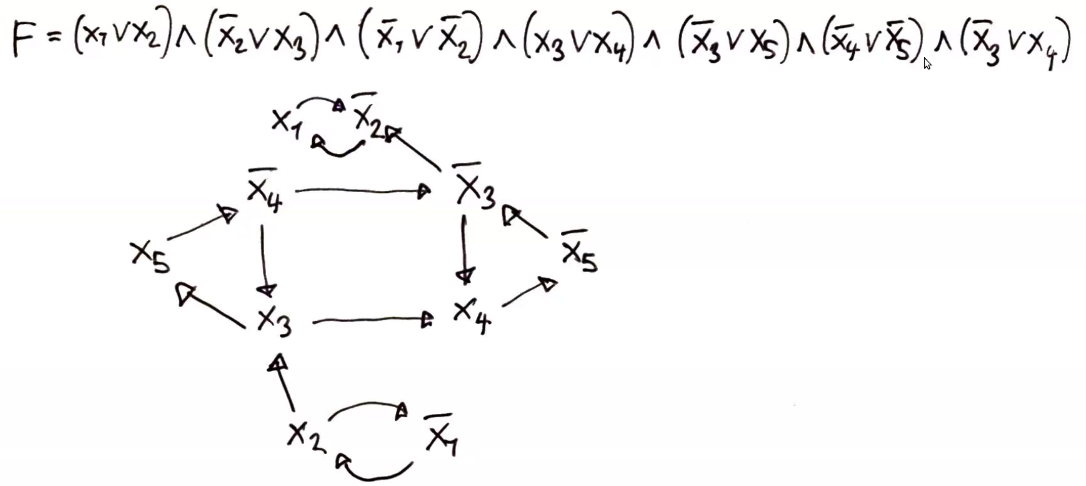
\includegraphics[scale=0.5]{2.png}\\
	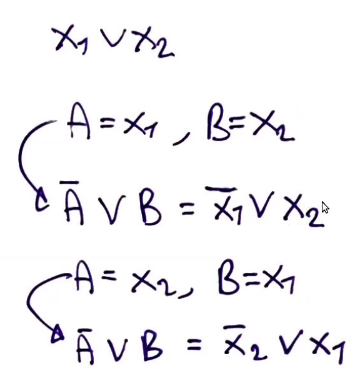
\includegraphics[scale=0.5]{3.png}\\
	$x_i \Rightarrow x_2$\\
	$x_2 \Rightarrow x_1$
\end{center}
Abbiamo definito un grafo orientato a partire dall'espressione logica. 2SAT sta in P, ma per passarci da SAT servono $2^n$ nuove clausole, rendendo la riduzione esponenziale.\\
Se esiste un arco $l\rightarrow \overline{l}$ e non esiste $\overline{l} \rightarrow l $, allora $(l = tt \Rightarrow \overline{l} = tt$ assurdo$) \Rightarrow l = ff$\\
Se esiste $\overline{l} \rightarrow l $ e non esiste $l\rightarrow \overline{l}$ allora $(\overline{l} = tt \Rightarrow l = tt$ assurdo$) \Rightarrow l = tt$\\
Nel caso ci siano entrambi gli archi, sono incompatibili quindi non esiste nessun assegnamento a $l$, quindi la formula originale è insoddisfacibile.\\
Da questo si deduce l'algoritmo\\
Se nella stessa componente totalmente connessa di $G$ trovo sia $l$ che $\overline{l}$, allora $F$ non è soddisfacibile.\\
Qual è la complessità della ricerca di un componenti totalmente connesse di un grafo diretto? Kosaraju in $O(|E| + |V|)$
\paragraph{Maxcut $\leq$ Qubo} \begin{list}{}{}
	\item Maxcut: ho $G(V,E)$ indiretto voglio trovare taglio $A\cup B = V$ che massimizza il numero di archi da $A$ a $B$.
	\item Quadratic Unconstraint Binary Optimization: assegnamento a variabili binarie $x_1,\ldots,x_n$ che massimizzi una formula del tipo $\textsl{max}\sum_{i,j} (b_ix_i + a_{ij}x_ix_j)$
\end{list}
Massimizzare distanza oggetti connessi da archi: se $x$ oggetto in A e $x$ connesso a $y$ allora voglio evitare di prendere $x$, così da evitare di prendere anche $y$. Ricorda lo xor.
%TODO tabella di verità
Algebra di Bool $x_i$ xor $x_j = x_i + x_j - 2x_ix_j$\\
$\textsl{max}\sum_{(i,j)\in E}(x_i + x_j - 2x_ix_j)$
\begin{list}{}{}
	\item $x_1 = 1$ allora $i \in A$
	\item $x_i = 0$ allora $i \in B$
\end{list}
\paragraph{CRICCA $\leq$ NodeCover}
\begin{list}{}{}
	\item CRICCA: dato un $G=(V,E)$ e $k$, ci chiediamo se esiste CRICCA con almeno $k$ vertici in $G$ (chiamando la CRICCA $K$)
	\item NodeCover (Cover): sottoinsieme vertici $C\subseteq V$ tali che per ogni arco $(u,v)\in E$ di G o $u\in C$ o $v\in C$
\end{list}
Si definisce un altro grafo a partire da $G$ che è il grafo complementare: stesso insieme di vertici ma insieme degli archi è il complementare dell'insieme dato (cioè, ho un arco $(u,v)\in \overline{E} \Leftrightarrow (u,v)\not\in E$)\\
Esiste una CRICCA con $k$ nodi in $G \Leftrightarrow$ esiste un NodeCover con al più $n-k$ nodi in $G'$ con $n = |V|$\\
Si osserva che se un certo arco sta negli archi che coinvolgono gli elementi della cricca, che è sottoinsieme di $E$, significa che quell'arco non può stare in $\overline{E}$ cioè $(u,v)\in E_K\subseteq E_G \Rightarrow (u,v)\not\in \overline{E}$\\
Quindi $(u,v)\not\in E \Rightarrow (u,v)\in \overline{E}$ allora $\overline{(u\in V_K \wedge v \in V_K)}$ quindi o $u \in V - V_K$ o $v in V - V_K$ con $|V-V_K|\leq n-k$\\
Devo trovare che in $G'$ i nodi rimasti sono collegati tra loro (quindi CRICCA).
\end{document}